\documentclass[11pt,a4paper,openany ]{book}
\makeatletter
\title{MEMOIRE}
\makeatletter
\newcommand{\crossout}[1]{%
\begingroup
\settowidth{\dimen@}{#1}%
\setlength{\unitlength}{0.05\dimen@}%
\settoheight{\dimen@}{#1}%
\count@=\dimen@
\divide\count@ by \unitlength
\count0=20 \count4=\count@\\
\loop
\count2=\count0 % keep a copy
\divide\count2\count4 \multiply\count2\count4
\ifnum\count2<\count0
\advance\count0 -\count2 % the remainder
\count2=\count0
\count0=\count4
\count4=\count2
\repeat
\count0=20 \divide\count0\count4
\count2=\count@ \divide\count2\count4
\begin{picture}(0,0)
\put(0,0){\line(\count0,\count2){20}}
\put(0,\count@){\line(\count0,-\count2){20}}
\end{picture}%
#1%
\endgroup
}
\makeatother
\newcommand\independent{\protect\mathpalette{\protect\independenT}{\perp}}
\def\independenT#1#2{\mathrel{\rlap{$#1#2$}\mkern2mu{#1#2}}}

\makeatletter % No page counter for \part
\renewcommand\part{%
	\if@openright
	\cleardoublepage
	\else
	\clearpage
	\fi
	\thispagestyle{empty}%   % Original »plain« replaced by »emptyx
	\if@twocolumn
	\onecolumn
	\@tempswatrue
	\else
	\@tempswafalse
	\fi
	\null\vfil
	\secdef\@part\@spart}
\makeatother
% ------------------------------
% PACKAGES DE BASE
% ------------------------------
\usepackage[dvipsnames]{xcolor}
\usepackage[utf8]{inputenc} 
\usepackage[T1]{fontenc} 
\usepackage{lmodern} % Police vectorielle
%\usepackage[sc]{

%\usepackage{kpfonts}%  for math    
%\usepackage{libertine}%  serif and sans 
%\usepackage[scaled=0.85]{beramono}%% mono

\usepackage[english]{babel}
\usepackage[a4paper]{geometry}
\usepackage{graphicx}
\usepackage{caption}
\usepackage{csquotes}
\usepackage{subcaption}
\usepackage{pdfpages}
\usepackage[flushleft]{threeparttable}
\usepackage{multirow}
\usepackage{footnote}
\makesavenoteenv{array}
\usepackage[bottom]{footmisc}
\usepackage{tabularx, booktabs}
\newcolumntype{Y}{>{\centering\arraybackslash}X}
\usepackage{listings}
\newcommand{\cmark}{\ding{51}}%
\newcommand{\xmark}{\ding{55}}%
\newcolumntype{C}[1]{>{\centering\let\newline\\\arraybackslash\hspace{0pt}}m{#1}}
\usepackage{longtable}

%\usepackage{titlesec}
%\titleformat{\chapter}[hang]{\bf\huge}{\thechapter}{2pc}{}
%\titlespacing*{\chapter}{0pt}{-1.5cm}{20pt}
\usepackage{sidecap}
\usepackage{pdflscape}
\usepackage{wrapfig}
\usepackage{listings}
\usepackage{babel,blindtext}
\usepackage{lipsum}
%\usepackage{slashbox}
\usepackage{dashrule}
\usepackage{hhline}
\usepackage{color}
%\usepackage{subfig}
\usepackage{graphicx}
\usepackage{subcaption}
%-------------------------------
% MATH
% ------------------------------
\usepackage{amsmath} % Les math
\makeatletter
\let\reftagform@=\tagform@
\def\tagform@#1{\maketag@@@{(\ignorespaces\textcolor{blue}{#1}\unskip\@@italiccorr)}}
\renewcommand{\eqref}[1]{\textup{\reftagform@{\ref{#1}}}}
\makeatother
\usepackage{amssymb} % Symboles math
\usepackage{esvect} % Vecteurs
\usepackage[amssymb]{SIunits}
\usepackage{eurosym}
\usepackage{mathrsfs}
\usepackage{dcolumn}
\usepackage{pifont}
\usepackage{amsthm}
\usepackage[breaklinks,colorlinks]{hyperref}
\hypersetup{
colorlinks=true,linkcolor=blue,%citecolor=CornflowerBlue,naturalnames=true,hypertexnames=false,
	filecolor=magenta,      
	urlcolor=cyan,
	citecolor=ForestGreen,
}
\usepackage{etoolbox}



\newtheorem{exe}{Theorem}
\setcounter{exe}{-1}


\usepackage[ruled,vlined]{algorithm2e}
\usepackage{mathtools}

\newcommand{\expect}{\operatorname{E}\expectarg}
\DeclarePairedDelimiterX{\expectarg}[1]{[}{]}{%
	\ifnum\currentgrouptype=16 \else\begingroup\fi
	\activatebar#1
	\ifnum\currentgrouptype=16 \else\endgroup\fi
}

\newcommand{\innermid}{\nonscript\;\delimsize\vert\nonscript\;}
\newcommand{\activatebar}{%
	\begingroup\lccode`\~=`\|
	\lowercase{\endgroup\let~}\innermid 
	\mathcode`|=\string"8000
}




\makeatletter

% Patch case where name and year are separated by aysep
\patchcmd{\NAT@cite}
{\@cite\NAT@hyper@{%
		\NAT@nmfmt{\NAT@nm}%
		\hyper@natlinkbreak{\NAT@aysep\NAT@spacechar}{\@citeb\@extra@b@citeb}%
		\NAT@date}}
{\@cite\NAT@nmfmt{\NAT@nm}%
	\NAT@aysep\NAT@spacechar\NAT@hyper@{\NAT@date}}{}{}

% Patch case where name and year are separated by opening bracket
\patchcmd{\NAT@cite}
{\@cite\NAT@hyper@{%
		\NAT@nmfmt{\NAT@nm}%
		\hyper@natlinkbreak{\NAT@spacechar\NAT@@open\if#1\else#1\NAT@spacechar\fi}%
		{\@citeb\@extra@b@citeb}%
		\NAT@date}}
{\@cite\NAT@nmfmt{\NAT@nm}%
	\NAT@spacechar\NAT@@open\if#1\else#1\NAT@spacechar\fi\NAT@hyper@{\NAT@date}}
{}{}

\makeatother

\usepackage{datetime} 
\usepackage{bm}
\usepackage{scalerel,stackengine}
\usepackage{pbox}
\usepackage{vmargin}            
\setmarginsrb{2,5cm}{2,7cm}{2,5cm}{2,5cm}{0cm}{1cm}{0cm}{1cm}
\rmfamily
%\DeclareFontShape{T1}{lmr}{b}{sc}{<->ssub*cmr/bx/sc}{}
%\DeclareFontShape{T1}{lmr}{bx}{sc}{<->ssub*cmr/bx/sc}{}

\DeclareMathOperator*{\argminA}{arg\,max} % Jan Hlavacek
\DeclareMathOperator*{\argminB}{argmax}   % Jan Hlavacek
\DeclareMathOperator*{\argminC}{\arg\max}   % rbp

\newcommand{\argmaxD}{\arg\!\max} % AlfC

\newcommand{\argminE}{\mathop{\mathrm{argmin}}}          % ASdeL
\newcommand{\argminF}{\mathop{\mathrm{argmin}}\limits} 

\usepackage{fancyhdr}
\usepackage{afterpage}
\fancypagestyle{plain}{\fancyhf{}}
\pagestyle{fancy}
\fancyfoot{}
\cfoot{\thepage}
\fancyhead[RO,LE]{\thepage}
\fancyhead[LO]{\leftmark}
\fancyhead[RE]{\rightmark}
\renewcommand{\headrulewidth}{.6pt}
\pagenumbering{roman}
\newcommand{\bib}{\par\noindent\hangindent=0.5 true cm \hangafter=1}

\makeatletter  % rm pg number in bottom
\let\@oddfoot\@empty
\let\@evenfoot\@empty
\makeatother
\usepackage{appendix}
%\usepackage[style=apa,backref=true,backend=biber,natbib=true,hyperref=true]{biblatex} 


%\addbibresource{zotero.bib.bib}
\usepackage{natbib}
\bibliographystyle{plainnat}
\setcitestyle{authoryear,open={(},close={)}}

%\bibliographystyle{abbrvnat}
%\setcitestyle{square}
%\setcitestyle{authoryear, open={[},close={)]}}
%\usepackage{apacite}
%\usepackage{cite}
%\usepackage[backend=biber]{biblatex}
\usepackage{bbm}
\usepackage{enumitem}
\usepackage{minitoc}

\newtheorem{theorem}{Theorem}[chapter]
\newtheorem{corollary}{Corollary}[theorem]
\newtheorem{lemma}[theorem]{Lemma}
%\theoremstyle{definition}
\newtheorem{definition}{Definition}[chapter]
%\renewcommand*{\proofname}{\boxed{Proof}}
\usepackage{tcolorbox}
\usepackage{adjustbox}
\usepackage{dashbox}


\newcommand{\abbrlabel}[1]{\makebox[3cm][l]{\textbf{#1}\ \dotfill}}
\newenvironment{abbreviations}{\begin{list}{}{\renewcommand{\makelabel}{\abbrlabel}}}{\end{list}}


\usepackage{tikz}
\usetikzlibrary{matrix,chains,positioning,decorations.pathreplacing,arrows}
%\defbeamertemplate{itemize item}{tikzarrow}{\tikz{\node[single
%		arrow,scale=0.2,inner sep=2ex,fill] at (0,0) {};}}

\tikzset{myarrow/.style={
		draw,
		fill=Emerald,
		single arrow,
		minimum height=5.5ex,
		single arrow head extend=1ex
	}
}
\newcommand{\arrowright}{%
	\tikz [baseline=-1ex]{\node [myarrow,rotate=0] {};}
}
\setlength{\parskip}{.3em}
\begin{document}
\thispagestyle{empty}
\begin{center}
	{\LARGE    UNIVERSITE CATHOLIQUE DE LOUVAIN} \\
	\vspace{0.2cm}
	{\large FACULTE DES SCIENCES} \\
	\vspace{0.2cm}
	{\Large ECOLE DE STATISTIQUE, BIOSTATISTIQUE \\
		\vspace{0.1cm}
		ET SCIENCES ACTUARIELLES }\\
\end{center}
\vfill

%\begin{figure}[H]
\begin{center}  \hspace*{-10mm} 
	
\includegraphics[height = 3.5cm]{lsba.jpg}
\end{center}
%\end{figure}


\vfill


\begin{center}
	{\Large \textsc{Temporal analysis of the evolution of extreme values using climatological data}}
	
\end{center}


\vfill

\begin{center}[]
	\begin{minipage}[c]{.45\linewidth}
		\begin{tabular}{ll}
			\vspace{0.2cm}
			Promoteur : & Johan \textsc{Segers} \\
			\vspace{0.2cm}
			Lecteurs : & Anna \textsc{Kiriliouk}\\
			\vspace{0.2cm}
			& Michel \textsc{Crucifix}
		\end{tabular}
	\end{minipage} \hfill
	\begin{minipage}[c]{.45\linewidth}
		\begin{tabularx}{\linewidth}{p{\textwidth}}
			Mémoire présenté en vue de \hbox{l'obtention} du \\   \vspace{0.1cm} Master en statistiques, orientation générale \\   \vspace{0.1cm} par :
			\textbf{Antoine \textsc{Pissoort}}
		\end{tabularx}
	\end{minipage}
\end{center}

\vspace{1,5cm}



\begin{center}
	{\large Juin 2017}
\end{center}

\newpage

\dominitoc
\tableofcontents
\newpage
\thispagestyle{empty}
\listoffigures
\thispagestyle{empty}

\newpage


%\centering
\topskip0pt
\vspace*{\fill}
\section*{\centering Abstract}
\begin{tcolorbox}%[colback=SeaGreen!75!white]
This thesis aims to analyse extreme temperatures from Uccle and assess their nonstationarity.% trend in the location parameter of the temperatures assessing the climate warming. 
 After having proven it by hand of splines's deriatives, we will do it by hand of the Extreme Value Theory (EVT)  that there is indeed an upward trend in the location parameter of the temperatures assessing the climate warming. First of all, we will do introductory analysis of the trend... and we will discover that..  Then we will go through with EVT by defining and presenting the usual methods such as GEV or POT. 

Regarding the computations, we took advantage of a high-level language (c++) to make our analysis efficient and also made use of parallel computing to decrease computation time for time consuming...
\thispagestyle{empty}
\end{tcolorbox}
\thispagestyle{empty}
\vspace*{\fill}



%\afterpage{\cfoot{\thepage}}


\newenvironment{acknowledgements}%
{\cleardoublepage\thispagestyle{empty}\null\vfill\begin{center}%
\bfseries Acknowledgements\end{center}}%
{\vfill\null}
\addcontentsline{toc}{chapter}{Acknowledgements}%
\begin{acknowledgements}
	\textit{I would first like to thank my thesis supervisor Johan Segers for all his help and his guidance during this whole year. The repeated appointments we have had   }
	\newline
	
	\textit{I also would like to thank the "Institut Royal de Météorologie" (IRM) of Belgium for his help and his guidance but also for his provided quality datasets.}
	\newline
	
	\textit{Finally, I want to thank my family and my friends, but also Bernadette for her support and all the time I have spent  writing in her room for my thesis but also during my whole academic studies.}
	
\end{acknowledgements}

%\newpage


\chapter*{List of Abbreviations}
\addcontentsline{toc}{chapter}{List of Abbreviations}
For convenience, we place a list of all the abbreviations we will use in the text. However, these will always be defined in their first occurrence into the text.\\

\begin{center}
\begin{abbreviations}
	\item [df]\label{df}  distribution function
	\item[EVI] Extreme Value Index ($\xi$)
	\item[EVT] Extreme Value Theory
	\item[GEV] Generalized Extreme Value
	\item[GPD] Generalized Pareto Distribution (function)
	\item[MCMC] Marko Chain Monte Carlo
	\item[MH] Metropolis-Hastings (algorithm)
	\item[TN] Temperature miNimum
	\item[TX] Temperature maXimum
	
\end{abbreviations}
\end{center}


%\chapter*{Acknoledgment}


\addcontentsline{toc}{chapter}{Introduction}
\chapter*{Introduction}
	%Presentation of the Analysis }
\pagenumbering{arabic}
\thispagestyle{empty}

%\pagestyle{myheadings}



Unlike his counterparts ( see for example credit risk analysis, financial applications,...), the extreme value analysis applied on the broad environemental area like here for the meteorological data, has strong impacts on the people lives 

An important question is still whether climate changes caused by anthropogenic activities will change the intensity and frequency of extreme events \cite{milly_climate_2008}.

The problem we are here facing in climate change evidence is that of le lack of past data to compare with her

Also, for such an analysis, the number of parameters to take into account is considerable (and tend to infinity)  

Can make a parallelism with Chaos Theory and the well-known butterfly effect which have strong applications in weather models\newline

We highly expect the climate change to affect the extreme weather  \newline

[extremes in climate change p.347]


It has been proven that winter become warmer in context of RC. (see naveau,...)


\cite{kharin_changes_2006}


"The first myth about climate extremes, which has been purported by
researchers in climatology or hydrology, among them prominent names, is that
“extremes are defined as rare events” or similar. This myth is debunked by a simple
bimodal PDF (Fig. 6.12a). The events sitting in the tails of that distribution are not
rare" \cite[pp.257]{mudelsee_climate_2014}
\newline

Until now, studies on climate extremes that consider Europe have usually had a strong national signature
%(e.g. Herzog and Muller-Westermeier, 1997; Brunetti ¨ et al., 2001)
, or have had to make use of either a
dataset with daily series from a very sparse network of meteorological stations (e.g. eight stations in Moberg
et al. (2000)) or standardized data analysis performed by different researchers in different countries along the
lines of agreed methodologies (e.g. Brazdil et al., 1996; Heino et al., 1999) \cite{klein_tank_daily_2002}

\textbf{During this project, we will try a novel approach, that is to link directly theory and practice and hence present the concepts theoretically and then illustrate by one example retrieved from our application. Even if that could be difficult, we think this approach is advantageous for several reasons :} 

Extrapolation !!!! See p154 [statistical analysis of extreme book]



Voir effet de l'ilot de chaleur --> urbanisation sur les tempés !

---> artificial warming on cities stations which were not(less) urbanized 100 years ago.

[In this thesis, efforts have been made to use power of (hyper)references into the 
text. While this not (yet ?...) usable in printed versions, the reader may feel more 
comfortable in a numeric version to more easily handle the vast amount of sections, 
equations, references, etc... and the links that are made between them.]

In this part, we will make use of some general methods to assess if there is indeed a trend in the maximum temperatures

In \hyperref[sec::1]{chapter \textbf{1}} we will present the method of block-maxima and derive the Generalized Extreme Value (GEV) distributions. In \hyperref[sec::2]{chapter \textbf{2}} we will .
In \hyperref[sec::3]{chapter \textbf{3}}
In \hyperref[sec::4]{chapter \textbf{4}} we will ..

Finally, we notice that this thesis will more concentrate on the block-maxima (GEV) methods (see \hyperref[sec::1]{chapter \textbf{1}}), i.e. to data relating to maxima over a period of 1 year. For example here in the introduction, or for the Bayesian analysis in \hyperref[sec::bayesian]{chapter \textbf{5}}.
\thispagestyle{empty}


\subsubsection*{Repository for the R code and Package}
An \textbf{R package} has been created and can be downloaded \url{https://github.com/proto4426/PissoortThesis}.

For your (best?) convenience, a folder has been created containing in the same repository containing all the scripts created during this thesis. It allows to reproduce all the results, and sometimes with more details, tables or plots. It can be retrieved directly in this page \url{https://github.com/proto4426/PissoortThesis/tree/master/Scripts-R}.

%\addcontentsline{toc}{section}{2 Presentation of the Analysis : Temperatures from Uccle}
\section{Presentation of the Analysis : Temperatures from Uccle}

The data used during this thesis have been gathered directly from the Institut Royal de Météorologie (IRM) 

%\addcontentsline{toc}{section}{Comparisons with freely available data}
\subsection{Comparisons with freely available data} 

A similar dataset is freely available on the internet\footnote{\url{http://lstat.kuleuven.be/Wiley/Data/ecad00045TX.txt}}. It was a project initially performed by the KMNI and which was used for example in \citet{beirlant_statistics_2006}. However, we were reticent to simply analyze these data as we know that it is hard to trust internet's data, even if they come from well-known "authorities". After having made all these comparisons analysis (see start of code...), we remark effectively that there are differences
in these two datasets, and hence large errors of measures can easily occur 
in unofficial data. It confirms the fact that is important to get reliable data if one wants to make reliable analysis. 
However, these differences tend to be much smaller when considering the "open shelter"
version ($54\%$ of equal measurements in closed shelter VS $14.4\%$ in the closed case). For this reason, we have confidence that this public datasets
is dealing with open shelter temperatures data.

However, for\textbf{ meteorological considerations}, it is always better to consider temperature's analysis in \textbf{closed shelters}. Indeed, thanks to gratefull advices from mr Tricot working for the IRM : 
\begin{itemize}
	\item It can
	\item It
\end{itemize}






\section{First Analysis}

As expected (~line 200 code local), from \ref{first_fig} we see that there is an upward trend for both (yearly) maxima and minima. However, we remark that this one is less pronounced for minima ( see figure \ref{seas4} in appendix \textbf{C}). That makes sense as (as mentioned above), the global warming is  


\begin{figure}
	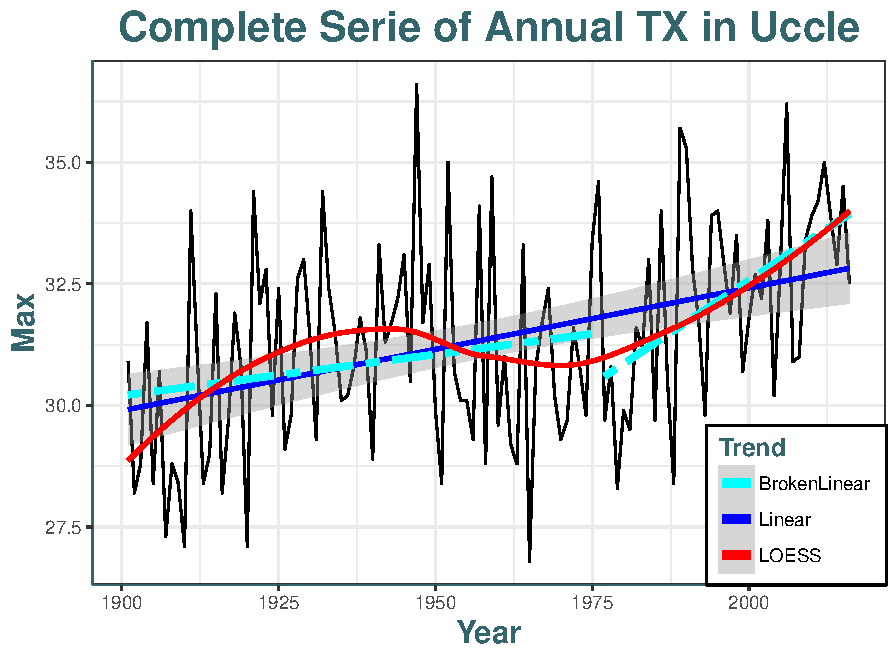
\includegraphics[width=.8\linewidth]{gg1.pdf}\caption{First plot representing the \textbf{yearly} maxima (\textbf{above}) and minima (\textbf{below}), shaded grey line representing the standard errors (and not a confidence interval ) of the linear trend, red line representing the polynomial nonparametric fit by LOESS.}\label{first_fig}
	\thispagestyle{empty}
\end{figure}


Add constraint to the broken linear trend to make it continuous : 

We will see that the decrease (around 1940 to 1970) is more from randomness than a real decrease (...)


TEST (statistic) for the Differences in trend !!!! !!!!!!!!

From the figure \ref{seas4}, we can already have some remarks : 

\begin{itemize}
	\item The drop in the series around 1950 to 1975 that is made visible by the LOESS estimator (red) is probably more due to a random effect than a real decrease or freezing of the maximum temperatures at this time. (to assessfofrmally if possible)
	\item  
\end{itemize}
\textbf{PUT the examples right in the place where it is mentioned in the theory.!} 
"As we have seen in section 2.1.1.... and in section 2.2.2......"

We must choose a block-length which is large enough for the limiting arguments supporting the GEV approximation (see (\ref{exttheom})) to be valid, either a large bias in the estimates could occur. For example, if this is too short, the maxima may be too close of each other to assume independence. But a large block-length implies less data to work with, and thus a large variance of the estimates.. So we must find a compromise between bias and variance.

TABLE with nested models (gumbel, GEV, + linear trend, etc etc)

From figure \ref{seas4} in appendix \textbf{C}, we can remark that

The code which provide all the tools to retrieve the presented results are left in appendix, but in the numeric version only be cause it is very heavy. this also enables you to get all insights (..)



\section*{GAM and splines}

\textbf{Simultaneous} confidence intervals :  Following \citet[section 3, 4.9, 6.5]{ruppert_semiparametric_2003} which uses a simulation-based approach to generate a simultaneous interval
\citet{marra_coverage_2012}

From the pointwise confidence intervals we can say that (example) $f(1980)$ has $95\%$ chance to lie within (-1,0) (say) and $f(2000)$ has also $95\%$ to lie within (0.2,1.2) BUT it is a fallacy to say simultaneously that both are contained in these intervals at the same time with .95 confidence. \citet[section 6.5]{ruppert_semiparametric_2003}


We can see that only the 2 increasing periods from the start and at the end of the series are significant, while the decreasing period from... (see the red line) is more likely to be the subject of randomness. Moreover, we remark that the 

Note that we will see further in the text (section \ref{bayes_cred_int} ) more explanations about the bayesian credible intervals.


After having... we will now go through with the more specific subjec of this thesis, that is the extreme value analysis.


\begin{center}
\part{Theoretical Framework : \qquad Extreme Value Theory}
\end{center}
%\pagestyle{fancy}

\setcounter{mtc}{3}
\chapter{Method of Block-Maxima} \label{sec::1}
\minitoc
%\newpage
 \vspace{1.5cm}

There are two approaches, the block-maxima  and the peaks-over-threshold approach (see 
\hyperref[sec::2]{section \textbf{2}}) yielding to different extreme value distribution. 
The former aims at while the latter models the...

In this section, we will present the basics of EVT and we will consider a 
\textit{block-maxima approach}. After defining some useful concepts in 
\hyperref[sec::1.1]{section \textbf{1.1}}, we will

\thispagestyle{empty}
\newpage
\section{Preliminaries}\label{sec::1.1}

Some useful definitions to start with !!
\theoremstyle{definition}
\begin{definition}[Similar distribution functions]\label{similardf} We say that two distributions functions $G$ and $G^*$ are \emph{\textbf{similar}} or are of the \emph{\textbf{same type}}
	if, for constants $a>0$ and $b$
	\begin{equation}\label{simm}
	G^*(az+b)=G(z), \ \ \ \ \ \ \forall z,
	\end{equation}
\end{definition}
which means that the distributions differ only in location and scale. 
In the sequel, the concept of \emph{similar} distributions will be useful to derive the three different families of extreme value distributions from other distributions of the \emph{same type}.
This is directly linked with max-stable process that we will define...

\begin{definition}[Max-stability] \label{maxstab}
	\emph{From \cite{leadbetter_extremes_1983} or \cite{resnick_extreme_1987}}, we say that a distribution $G$ is \emph{\textbf{max-stable}} if, for each $n\in\mathbb{N}$
	
	
	\begin{equation}
	G^n(a_nz+b_n)=G(z), \ \ \ \ \ \ \ n=2,3,...
	\end{equation}
	
	for some constants $a_n>0$ and $b_n$.
\end{definition}
In other words, taking powers of $G$ results only in a change of location and scale. \ref{stat modelling..course slide Coles} This concept will be closely connected with the extremal limit laws in the following ().
However, max-stable process are more used in a multivariate setting, see for example \citet{} for an introduction.

\emph{Min-stability} can easily be found by complement, see for instance \citet[pp.23]{ reiss_statistical_2007}.

\iffalse
\begin{definition}[Min-stability]
	Anageously, from \citet[pp.23]{ reiss_statistical_2007}, we say that a distribution function $G$ is \emph{\textbf{min-stable}} if 
	
\begin{equation}
\text{\emph{Pr}} \big\{X_{(1)}> d_n+c_nz \big\}=\bar{G}^n(d_n+c_nz)=\bar{G}(z),
\end{equation}
	where $c_n=a_n$, $d_n=-b_n$ and $X_{(1)}$ the minimum of the sample of size n, see (\ref{min}).
\end{definition}
\fi

\paragraph{Principles of stability}
% course slides 18 coles 
Behind all the principles about Extreme Value Theory that will be covered during this thesis, will be influenced by the principle of \emph{stability}.
\newline

As this will be .. in the following, we think useful to define precisely the concept of \emph{non-degenerate distribution functions}.
\begin{definition}[Non-degenerate distribution functions]
	We say that a distribution function is \emph{\textbf{non-degenerate}} if 
\end{definition}

We illustrate this by the most common theorem in statistics, the \emph{Central Limit Theorem} (CLT) which plays typically with the empirical mean $\bar{X}_n=n^{-1}\sum_{i=1}^nX_i$. We know that (..) $\bar{X}_n$ converges to the true mean $\mu$ in probability(?) and thus in distribution, that is to a non-random single point, i.e. to a \emph{degenerate} distribution 

\begin{equation*}
\text{Pr}\big\{\bar{X}_n\leq x\big\}= \begin{cases}
\ 0, \ \ \ \ \ \ \ \ \ \ \ \ x<\mu; \\
\ 1, \ \ \ \  \ \ \ \ \ \ \ \ x\geq \mu. 
\end{cases}
\end{equation*}
That is not very useful, in particular for inferential purposes.

For this reason, CLT aims at finding a non-degenerate limiting distribution for $\bar{X}_n$, after allowance for normalization by sequences of constants. We will state it in his most basic form :

\begin{exe}[Central Limit Theorem] 
	Write\footnote{We adopt this notation w.l.o.g. in the following, if there is no confusion possible. It is the same as $X_1,\dots,X_n$} $\{X_i\}$ as a sequence \emph{(or "stochastic process"?!.. Check if written like this is fine ! for the following too)}  of n iid random variables with $E(X^2_i)<\infty$. Then, $\text{as} \ n\rightarrow\infty$,
	
	\begin{equation*}
	\sqrt{n}(\bar{X}_n-\mu)\stackrel{d}{\longrightarrow}N(0,\sigma^2),
	\end{equation*}
	where $\mu=E(X_i)$ and $\sigma^2=V(X)>0$. $d$ means convergence in distribution and the reader may refer to \hyperref[convconc]{\emph{appendix\textbf{ A.}}} for a useful short review of most important concepts of convergence for EVT.
\end{exe}
Then, by a proper choice of some normalizing constants, $\mu$ and $\sqrt{n}$ (as location and scale parameters respectively), we find the non-degenerate Normal distribution in the limit for the empirical mean $\bar{X}_n$. 

With the same logic, we find that this is the same for the distribution of $X_{(n)}$ 
\begin{equation}
\displaystyle{\lim_{n \to \infty}}\text{Pr}\big\{X_{(n)}\leq x\big\}=\displaystyle{\lim_{n \to \infty}}\text{Pr}\big\{X_i\leq x\big\}^n=\begin{cases}
\ 0, \ \ \ \ \ \ \ \ \ \ \  \ \ \ F(x)<1; \\ 
\ 1, \ \ \ \ \ \ \ \ \ \ \ \  \ \ F(x)=1.
\end{cases}
\end{equation}

That is, another degenerate distribution.
This is exactly what Extreme Value Theory aims to achieve for (typically) the maximum order statistics $X_{(n)}$, that is finding a non-degenerate distribution in the limit by means of normalization. This will be the main subject of the next sections.


\section{Extremal Types Theorem}




Introduced by Fisher and Tippett \cite{fisher_limiting_1928}, later revised by \cite{gnedenko_sur_1943} and finally streamlined by \cite{De_on_1970}, the \emph{extremal types} theorem is very important for its applications. We remind the distribution of maxima is $\text{Pr}\big\{X_{(n)}\leq x\big\}=F^n(x)$, from \ref{maxdist} in \hyperref[appA]{appendix \textbf{A}}. It states the following:

\begin{theorem}[Extremal types theorem] \label{extthm}
	If the distribution of partial maxima of an iid sequence of  random  variables  with  common  (unknown)  distribution F, say, $X_{(n)}$, properly normalized, converges to a non-degenerate ( see ...) limiting distribution G, i.e.
	\begin{equation} \label{exttheom}
	\displaystyle{\lim_{n \to \infty}}\text{\emph{Pr}}\Big\{ a_n^{-1}(X_{(n)}-b_n)\leq z\Big\}=F^n(a_nz+b_n)
	= G(z), \ \ \ \ \ \ \ \ (\forall z\in\mathbb{R})),
	\end{equation}
	
	and for some constants $a_n>0$, $b_n\in\mathbb{R}$.
\end{theorem}
[extreme value and cluster ana. of euro... clustering 2011]
, meaning that $F$ is said to be in the \textbf{domain of attraction}\footnote{?? We will more precisely define this concept in the next section.} of $G$, denoted by $F\in D(G)$.
This theorem considers an i.i.d. random sample, but it holds true if the original scheme 
being no longer i.d. still remains independent (we will present the stationary case in 
\hyperref[statio]{section \textbf{3.1}}). However, even the stationary assumption is often 
poor in practical applications (see for our applications in our case, the temperature....)
\cite{gomes_bootstrap_2015} (see application...) but we will handle that in \hyperref[nstatio]{section \textbf{3.2}} . with $G$ the \textit{Generalized Extreme Value} (GEV) distribution :

\begin{equation} \label{gevgen}
G(z)=\ \text{exp}\ \Bigg\{-\bigg[1+\xi\bigg(\frac{z-\mu}{\sigma}\bigg)\bigg]_+^{-\xi^{-1}}\Bigg\}:=G_{\xi}(z),
\end{equation}

from which we introduce the notation $y_+=\text{max}(y,0)$, denoting in the above that 
$\{z:1+\xi\sigma^{-1}(z-\mu)>0$\} to ensure the term in the exponential is negative and the 
distribution function converges to 1. We will use this notation in the following so it is important to remind that this yields a vital condition(?). This will 
define the endpoints of the different distribution functions from the values of the shape 
parameter, that is \{$\xi>0$; $\xi<0$; $\xi=0$\}, more details will be provided in next 
section . Moreover,  $-\infty<\mu,\xi<\infty$ and $\sigma>0$ with 
$\mu,\sigma$ and $\xi$ being the three parameters of the model characterizing location, 
scale and shape respectively.

We think important to point out that here, the location parameter $\mu$ does not represent
the mean as in the classic statistical view, but does represent the “center” of the distribution, and the scale parameter
$\sigma$ is not the standard deviation, but does govern the “size” of the deviations around $\mu$. This can already be pointed out on figures in appendix where we demonstrate for little variations of the parameters.
\newline

From \cite{coles_introduction_2001}, we introduce an important theorem in Extreme Value Theory and that has many implications. This theorem simply says the following :

\begin{theorem}\label{max-gev} For any distribution function $F$,
	
	\begin{equation}
	F \ \emph{\text{is \emph{max-stable}}}\ \Longleftrightarrow \ F \emph{\text{ is GEV}}.
	\end{equation}
\end{theorem}
Any distribution functions that are \emph{max-stables} (see \hyperref[maxstab]{ definition \textbf{1.2}}) are also GEV (\hyperref[extthm]{theorem \textbf{1.2}}), and vice-versa.
To gain interesting insights of the implications of this theorem, we think useful to give a proof but only for the "$\Leftarrow$" as the converse requires too much mathematical backgrounds.

\begin{proof}[\boxed{\emph{Proof :}}\nopunct ]
\ \ \	\begin{itemize}
    \item	If $a_n^{-1}(X_{(n)}-b_n)$ has limit distribution $G$ for large $n$ as in (\ref{exttheom}), then
	
	\begin{equation*} \label{gevproof1}
	\text{Pr}\Big\{ a_n^{-1}(X_{(n)}-b_n)\leq z\Big\}\approx G(z).
	\end{equation*}
	
	Hence for any integer $k$, since $nk$ is large, we have
	
	\begin{equation} \label{bigup}
	\text{Pr}\Big\{ a_{nk}^{-1}(X_{(n)k}-b_{nk})\leq z\Big\}\approx G(z).
	\end{equation}
	
	\item Since $X_{(n)k}$ is the maximum of $k$ variables having identical distribution as $X_{(n)}$,
	
	\begin{equation} \label{bigup1}
	\text{Pr}\Big\{ a_{nk}^{-1}(X_{(n)k}-b_{nk})\leq z\Big\}=\Big[\text{Pr}\big\{ a_{nk}^{-1}(X_{(n)}-b_{nk})\leq z\big\}\Big]^k,
	\end{equation}
	
	giving two expressions for the distribution of $M_n$, by (\ref{bigup}) and (\ref{bigup1}) :
	
	\begin{equation*}\label{gevproofl}
	\text{Pr}\{X_{(n)}\leq z\}\approx G\Big(a_n^{-1}(z-b_n)\Big) \ \ \ \ \text{and} \ \ \ \ \text{Pr}\{X_{(n)}\leq z\} \approx G^{1/k}\Big(a_{nk}^{-1}(z-b_{nk})\Big).
	\end{equation*}
	\item It follows that $G$ and $G^{1/k}$ are identical apart from location and scale coefficients. 
	Hence, $G$ is \emph{max-stable} and therefore GEV. This gives proof of the \textbf{extremal 
	types theorem}, \ref{extthm}.
  \end{itemize}
\end{proof}

\section{Characterization of the GEV distributions : 3 Types}
...

The quantity $\xi\in\mathbb{R}$ in (\ref{gevgen}) is called the \emph{extreme value index} (EVI) and is at the center of the analysis in extreme value theory. It determines, in some degree of accuracy, the type of the underlying distribution.
Hence, from this general definition of the GEV distribution (\ref{gevgen}), we can directly retrieved three principal classes of EV distributions, from their \emph{standard form}, in the \emph{$\alpha$-parametrization}, with $\alpha=\xi^{-1}$ (just show in the $\xi$ param. ? for convenience) :

\begin{equation}\label{gumb}
\boxed{\textbf{\text{I}}}\ \   G_1(z)= 
\exp\{-e^{-z}\}, \ \ \ \ \ \ -\infty<z<\infty.    
\end{equation}


\begin{equation} \label{frech}
\boxed{\textbf{\text{II}}} \ \ G_{2,\alpha}(z)=
\begin{cases}
\ 0, \ \ \ \ \ \ \ \ \ \ \ \ \ \ \ \ \ \ \ \ \ \ \ \ \ z\leq 0; \\
\ \exp\{-(z)^{-\alpha}\}, \ \ \ \ \ \ \ \ \ z>0,\ \alpha>0.    
\end{cases}
\end{equation}

\begin{equation} \label{weib}
\ \ \boxed{\textbf{\text{III}}} \ \ G_{3,\alpha}(z)=\begin{cases}
\ \exp\big\{-(-z)^{\alpha}\big\}, \ \ \ \  z>0,\ \alpha>0?;     \\
\  1, \ \ \ \ \ \ \ \ \ \ \ \ \ \ \ \ \ \ \ \ \ \ \ z\geq 0.
\end{cases}
\end{equation}
\newline
[Faire tableau]

(mettre les indice aux fctions G + le shape parameter est "correct" ????)

The II and III can be reformulated (in the $\xi$-parametrization) as.....

\begin{equation}\label{GEVxineq0}
G_{\xi}(z)=\exp\Bigg\{-\bigg[1+\xi \bigg(\frac{z-\mu}{\sigma}\bigg)\bigg]_+^{-\xi^{-1}}\Bigg\}, \ \ \ \ \ \ \ \ \ \ \ \ \  \xi\neq 0,
\end{equation}

where we added explicitly the location and scale parameters $\mu$ and $\sigma$ in order to obtain the three \emph{extreme value distributions}, see for example \cite[pp.16]{reiss_statistical_2007} among others. The parameters are such that $ \sigma>0$ and $-\infty<\mu,\xi<\infty$.
This statement will hold for the rest of this thesis

By simply coming back in the $\xi$-parametrization by using $\xi=\alpha^{-1}$ in the above distribution functions,  all these three classes of extreme distributions can be expressed in the same functional form as special cases of this single three-parameter (Actually, there are just location and scale parameters in the type \textbf{I} extremal model in (\ref{gumb})  as $\xi\to 0$) distribution (\ref{gevgen}).
That is, when $\xi\rightarrow 0$ we retrieve the \textbf{type I} or \emph{Gumbel} family (\ref{gumb}) while $\xi >0$ and $\xi <0$ leads to the \textbf{type II}  or \emph{Fréchet} family and to the \textbf{type III} or \emph{Weibull} family, see (\ref{frech}) and (\ref{weib}) respectively. Both the Gumbel and Fréchet limiting distributions are unbounded (In fact, the Fréchet distribution has a finite left endpoint in $\mu-\sigma\xi^{-1}$, but this has no really interest here); that is, the upper endpoint tends to $+\infty$ while the Weibull distribution has a finite right endpoint in $\mu-\sigma\xi^{-1}$. In the following, we define the left and the right endpoint of a particular df $F$, respectively $_*x$ and $x_*$, by :
\begin{equation*}
_*x=\inf\{x:F(x)>0\}, \ \ \ \ \ \ \text{and} \ \ \ \ \  x_*=\sup\{x:F(x)<1\}.
\end{equation*}



\paragraph{Density}We give a representation of the density of these functions by considering the density of the GEV distribution (\ref{gevgen}), that is $g_{\xi}(z)=\frac{d G_{\xi}(z)}{dz}$ (we can assume absolute continuity). This is shown in in figure (\ref{gevdens}) for various shape parameters. We also give in appendix. \emph{Or: As the relation of the (density) distribution with the location and scale parameters is trivial, we do not illustrate that here. However, for the shape parameter it is a bit more subtil... and we let the figure}

For the case $\xi\neq0$, 
\begin{equation}\label{densgev}
g_{\xi}(z)=\sigma^{-1}\bigg[1+\xi\bigg(\frac{z-\mu}{\sigma}\bigg)\bigg]_+^{-\frac{1}{\xi}-1}\exp\Bigg\{-\bigg[1+\xi\bigg(\frac{z-\mu}{\sigma}\bigg)\bigg]_+^{-\xi^{-1}}\Bigg\},
\end{equation}
[table + two case for $Xi=0$ and $xi\ne 0$]
[appendix graphs for various location/scale parameter values ]

For the case $\xi=0$, we have 
\begin{equation} \label{gevdensxi0}
g_0(z)= \sigma^{-1}\exp\bigg\{-\bigg(\frac{z-\mu}{\sigma}\bigg)\bigg\}\exp\Bigg\{-\exp\bigg[-\bigg(\frac{z-\mu}{\sigma}\bigg)\bigg]\Bigg\},
\end{equation}

Note that the support varies equally as for the distribution functions wrt sign of $\xi$


%\begin{center}
\begin{figure}
	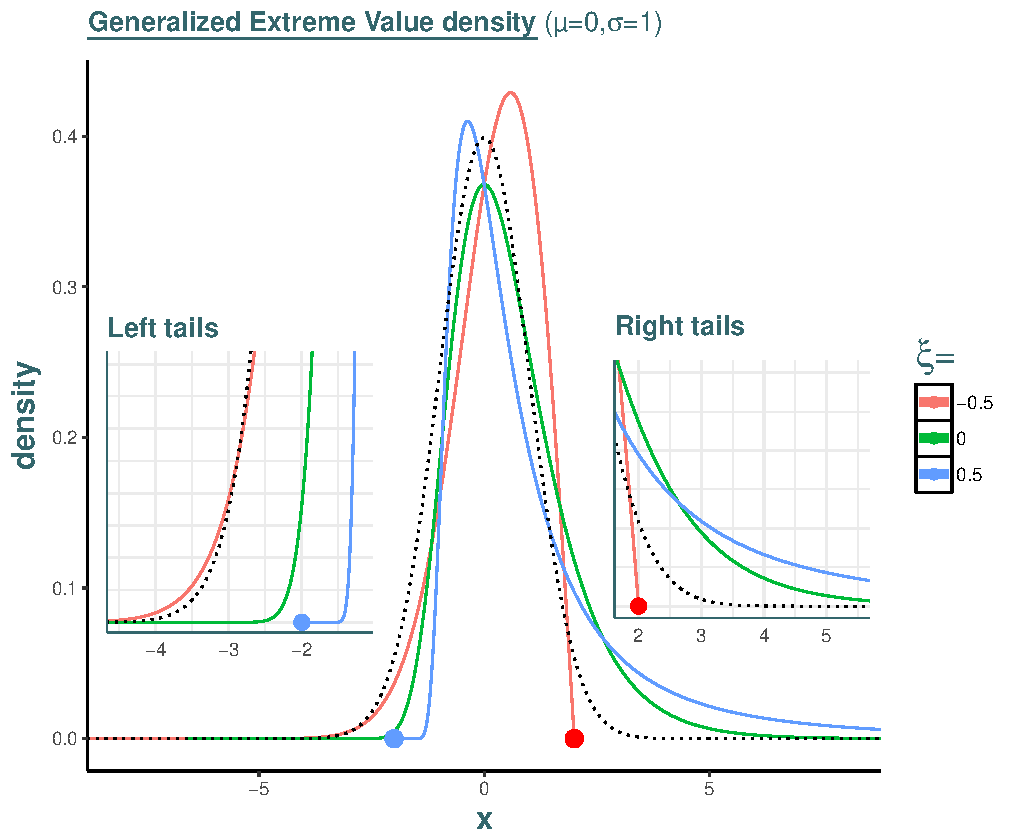
\includegraphics[width=0.85\textwidth, height = 0.7\linewidth]{gev3.pdf}\caption{GEV distribution with the normal in dotted lines and a zoom on the part of interest, the tails  ...}\label{gev3plot}
\end{figure}
%\end{center}




?? dernier graphe weibull
\newline
In some ways, some people will feel this was unfortunate, because now it is common for
people to model and fit the GEV without thinking very clearly about the
specific form of their data and distributions [Extremes, distribution, etc..] That is the 
reason why we think it can be useful to explain in the following some examples of how we 
can construct such extreme distributions for the three classes in concrete cases (see 
\hyperref[sec::appconcrete]{next section}), playing with the appropriate choice of 
sequences 
$a_n$ and $b_n$ to retrieve the pertaining distribution family.
%\newline



\section{Concrete applications : examples of convergence to GEV}\label{sec::appconcrete}

This is well not easy to find the sequences in practice.
\url{http://stats.stackexchange.com/questions/105745/extreme-value-theory-show-normal-to-gumbel/105749#105749}

\subsection*{Convergence to Gumbel distribution}
The \textbf{\underline{Type I}} or \textbf{Gumbel} distribution $G_1(x)$ can be retrieved by considering, for example,  a iid exponential distributed sequence $\{X_j\}$ of $n$ random variables, that is $X_j\stackrel{iid}{\sim}Exp(\lambda)$ and consider the largest of these values $X_{(n)}$ as defined earlier. By definition, we know $F(x)=1-\exp^{-x}$. Our goal is to find non-random sequences $\{b_n\}$, $\{a_n>0\}$ such that 
\begin{equation}
\displaystyle{\lim_{n \to \infty}}\text{Pr}\big\{ a_n^{-1}(X_{(n)}-b_n)\leq z\big\}=G_1(z).
\end{equation}
We can easily find that
\begin{equation*}
\begin{aligned}
\text{Pr}\big\{ a_n^{-1}(X_{(n)}-b_n)\leq z\big\}
&=\text{Pr}\{X_{(n)}\leq b_n+a_nz\} \\ &=\Big[\text{Pr}\{X_1\leq b_n+a_nz\}\Big]^n \\
&=\Big[1-\exp\big\{-\lambda(b_n+a_nz)\big\}\Big]^n,
\end{aligned}
\end{equation*}

from the iid assumption of the random variables and their exponential distribution.
Hence, by choosing  the sequences $a_n=\lambda^{-1}\log n$ and $b_n=\lambda^{-1}$ and reminding that% $\displaystyle{\lim_{n \to \infty}}(1+\frac{x}{n})^n=\exp(x)$,


\begin{equation*}
\begin{aligned}
\Big[1-\exp\big\{-\lambda(b_n+a_nz)\big\}\Big]^n 
& = \Big[1-\frac{1}{n}e^{-z}\Big]^n \ \ \ \ \ \ \ \ \ \ \ \ \ \ \ \ \ \ \ \ \ \ \ \ \ \scriptsize\text{\underline{Recall:}} \ \ %\begin{adjustbox}{minipage=0.2\textwidth,precode=\dbox} \scriptsize\displaystyle{\lim_{n \to \infty}}\Big(1+\frac{x}{n}\Big)^n=\exp(x)
%\end{adjustbox}
\boxed{\scriptsize\displaystyle{\lim_{n \to \infty}}\Big(1+\frac{x}{n}\Big)^n=\exp(x)} \\
& \stackrel{n\to\infty}{\longrightarrow} \exp(-e^{-z}):=G_1(z).
\end{aligned}
\end{equation*}
%\mathcenter

intro \cite{falk_laws_2011} somewhR

we find the the so-called standard \emph{Gumbel} distribution in the limit. 

We can show the same with iid standard normal random variables, $X_j\stackrel{iid}{\sim}N(0,1)$, with sequences $a_n=-\Phi^{-1}(1/n)$ and $b_n=1/a_n$. (see appendix [extremes, distributions  pdf] )

Typically, unbounded distributions like the Exponential and Normal (as well
as the Gamma, Lognormal, Weibull, etc.) whose tails fall off exponentially
or faster will have this same Gumbel limiting distribution for the maxima,
and will have medians (and other quantiles) that grow as $n\rightarrow\infty$ at the rate
of (some power of) $\log n$. This is typical example of light-tailed distribution (i.e., decays exponentially as defined in section \textbf{1.1}).

\subsection*{Convergence to Fréchet distribution}

The \textbf{\underline{Type II}} or \textbf{Fréchet-Pareto type} distrbution $G_2(x)$  ...

%[Practical analysis of extreme values p.51]
When starting with a sequence $\{X_j\}$ of $n$ iid random variables (block-maxima?) following a \textit{basic}(or \textit{generalized}, with scale parameter set to 1) Pareto distribution with shape parameter $\alpha\in (0,\infty)$, $X_j\sim Pa(\alpha$), we have that 

\begin{equation}
F(x)=1-x^{-\alpha}, \ \ \ \ \ \ \ \ \ \ \ \ \ \ x\in[1,\infty),
\end{equation}

so that we can write, by choosing appropriately $b_n=0$

\begin{equation*}
\begin{aligned}
-n\bar{F}(a_nz+b_n)
& =-n(a_nz+b_n)^{-\alpha} \\
& =\Big[Q(1-\frac{1}{n})\Big]^{\alpha}(a_n)^{-\alpha}(-z^{-\alpha}),
\end{aligned}
\end{equation*}

where $Q(1-\frac{1}{n})$ is the quantile function (see). Hence, it is easy to see that by setting the constant $a_n=Q(1-1/n)$ and keeping $b_n=0$, we have that 
\begin{equation*}
\text{Pr}\{a_n^{-1}X_{(n)}\leq z\}\rightarrow \exp (-z^{-\alpha}),
\end{equation*}
showing that for this particular values of the normalizing constants, we retrieve the Fréchet distribution in the limit from a strict Pareto distribution. The fact that $b_n$ is set to zero can be understood intuitively since for heavy-tailed distribution (see) such as the Pareto distribution, a correction for location is not necessary to obtain non-degenerate limit distribution. \cite[pp.51]{beirlant_practical_1996}


[see p.28 memoire other si ft autre exemple]


More generally, we can state the more general following theorem :
\begin{theorem}[Pareto-type distributions] ?? For the same choice of normalizing constants as above, that is $a_n=Q(1-\frac{1}{n})$ and $b_n=0$ and for any $x\in\mathbb{R}$, if
	
	\begin{equation}
	\begin{aligned}
	n[1-F(a_nx)]= \frac{1-F(a_nx)}{1-F(a_n)}\rightarrow x^{-\alpha} ,&&&&&&&&&&&& \text{ n}\to\infty
	\end{aligned}
	\end{equation}
	
	then we obtain the Fréchet distribution in the limit, or written formally "\emph{$\bar{F}$ is of Pareto-type}" or, more technically, "\emph{$\bar{F}$ is regularly varying with index -$\alpha$}".
\end{theorem}
We let the concepts of \textbf{regularly varying functions}, together with \textbf{slowly varying functions} be defined in appendix A.1 with some useful theorems and properties, according to \citet[pp.51-54]{beirlant_practical_1996} and supported by \citet[pp.49, 77-82]{beirlant_statistics_2006}.

\citet[pp.75]{beirlant_statistics_2006} !!!!

\subsection*{Convergence to Weibull distribution}

The \textbf{\underline{Type III}} or \textbf{Weibull} family (?) of distributions $G_3(x)$ are, for example, in the limit of $n$ iid uniform random variables $X_j\sim U[L,R]$ where $L$ and $R>L$ are both in $\mathbb{R}$  and denote respectively the Left and the Right endpoint of the domain of definition. We have by definition

\begin{equation*}
F(x)=\frac{x}{R-L}, \ \ \ \ \ \ \ \  \ \ x\in [L,R].
\end{equation*}
It is $=0$ for $x<L$,  $=1$ for $x>R$.
Assuming the general case ($[L,R]$ can be $\neq [0,1]$), we have for the maximum $X_{(n)}$
:
\begin{equation*}
\begin{aligned}
\text{Pr}\{a_n^{-1}(X_{(n)}-b_n)\leq z\}
&=\text{Pr}\{X_{(n)}\leq b_n+a_nz\} \\
& = \Big[1-\frac{R-b_n-a_nz}{R-L}\Big]^n, & & \text{if}\ \ \ L\leq b_n+a_nz\leq Rn, \\ 
& = (1+\frac{z}{n})^n\to e^z, & & \text{if} \ \ \  z\leq 0 \ \text{and} \ n>|z|.
\end{aligned}
\end{equation*}
When choosing $a_n=R$ and $b_n=(R-L)/n$, we find the unit Reversed Weibull distribution $We(1,1)$ in the limit as expected.
\newline

However, for inferential purpose, this is not of particular interest, because from the expression in \ref{exttheom}, we know that

\begin{equation} \label{convseq1}
a_n^{-1}(X_{(n)}-b_n)\stackrel{d}{\longrightarrow} G_{\xi,\mu,\sigma}(z), \ \ \ \ \ \text{as} \ n\rightarrow\infty.
\end{equation}
After some algebra, this leads to 
\begin{equation}\label{convseq2}
X_{(n)}\stackrel{d}{\longrightarrow} G_{\xi,\mu^*,\sigma^*}(z), \ \ \ \ \ \text{as} \ n\rightarrow\infty,
\end{equation}
with the sequences $a_n$ and $b_n$ being absorbed into the new location and scale parameters $\mu^*$ and $\sigma^*$. We can then ignore the normalizing constants in practical applications and fit directly the GEV in our set of maxima $X_{(n),k}$.
The pertaining estimated parameters will implicitly take the normalization into account, i.e. it will estimate $\mu^*$ and $\sigma^*$.
As also stated in..,  the shape parameter is invariant.

But what about the fact that $X_{(n)}$ non-normalized is degenerate (see intro) ?

\subsection*{Some Conditions/comments (?) (Continuity condition)}

As we have noticed in (?), $F$ needs certain conditions at its right endpoint $x_*$ for the limit to be convergent in (\ref{extthm}). The \emph{continuity condition} ensures that a discrete distribution cannot have a non-degenrate limit distribution as in (\ref{extthm}). Examples are well documented by  \citet{modelling_embrechts_1997}[pp.118-119] for the case of poisson, Geometric and negative binomial distribution. Thus, we cannot have a limit for these distributions.


\section{Maximum domain of attraction}

The preceding results can be more easily summarized and obtained when considering \emph{maximum domain of attraction} (MDA). The term "\emph{maximum}" is typically used to distinguish from \emph{sum-stable} distribution. As we study here only the maxima, there are no confusion possible in our work. We will then preferably write only \emph{domain of attraction} in the following for convenience, and thus consider these two names as synonyms.

\begin{definition}[Domain of attraction] We say that a distribution $F$ is in the (\emph{\textbf{maximum}}) \emph{\textbf{domain of attraction}} of an extreme value family $G_k$ \big(see (\ref{gumb})-(\ref{weib})\big), denoted by $F\in D(G_k)$, if there exist $a_n>0$ and $b_n\in\mathbb{R}$ such that the distribution
	of $a_n^{-1}(X_{(n)}-b_n)$ converges weakly (see \ref{conv_weak}) to $G_k$ where $X_{(n)}$ is as defined earlier with distribution $F$.
\end{definition}
The definition is well-defined in the sense that $F\in D(G_i)$ and $F\in D(G_j)$ implies $\xi_i=\xi_j$, writing by $\xi_k$ the extreme value index pertaining to the extreme value distribution $G_k$.

Before going further with the characterization of the three domains of attraction of our purpose, we think important to introduce a new theorem from Gnedenko \cite{gnedenko_sur la distribution_translated_1992}

\begin{theorem}[Convergence to Types Theorem]
	Let $F_n$ be a sequence of random variables converging weakly (see appendix A.1.1 ) to $F$. Let $a_n>0$ and $b_n\in \mathbb{R}$ such that $a_nF_n+b_n\Rightarrow F'$, where both $F$ and $F'$ are non-degenerate (see \ref{} ). Then, 
	
	\begin{equation*}
	a_n\to a \ \ \ \text{and} \ \ \ b_n\to b, \ \ \ \ \ \ \ \ \ a>0 \ \ \ \text{and} \ \ \ b\in\mathbb{R}.
	\end{equation*}
	
	Equivalently, if $G_n$, $G$, $G'$ are distribution functions with $G$, $G'$ being non-degenerate, and there exists $a_n,a'_n>0$ and $b_n,b'_n\in\mathbb{R}$ such that
	
	\begin{equation*} G_n(a_nx+b_n)\stackrel{d}{\to} G(x) \ \ \ \ \text{and} \ \ \ \  G_n(a'_nx+b'_n)\stackrel{d}{\to} G'(x),
	\end{equation*}
	
	at all continuity points of $F$, respectively $F'$, then there exists constants $A>0$ and $B\in\mathbb{R}$ such that 
	
	\begin{equation*}
	\displaystyle{\lim_{n \to \infty}} \ \frac{a_n}{a'_n}\to A, \ \ \ \ \ \ \ \ \displaystyle{\lim_{n \to \infty}} \frac{(b_n-b'_n)}{a'_n}\to B,
	\end{equation*}
	and $G'(Ax+B)=G(x) \ \forall x\in\mathbb{R}$. 
\end{theorem}

We have now all the necessary tools to  the pertaining domains of attractions. But, before proceeding, we would like to point out that the fact that the characterization of the first domain of attraction (Gumbel class)  is much more complex than the two following (Fréchet and Weibull class) and requires much more technicalities going beyond the scope of this thesis. Moreover, despite this class is important in theory, it is less relevant for our purpose of modelling extremes. It often requires other generalizations, for instance with additional parameters to surpass the issues of fitting empirical data. \cite{pinheiro_comparative_2015}
In the last paragraph, we will present the unified framework, the domain of attraction pertaining to the GEV distributions, which is a kind of summary for the three first domains of attraction presented.
\newline
In each of the characterization of the domains of attractions, we will present some of their most useful, necessary and sufficient conditions ... together with their \emph{von Mises conditions}, initially from \cite{} but revisited in \cite{falk_vonmises_1994}. These conditions are very important in practice and sometimes more intuitive because they make use of the \emph{hazard function}, defined by, for sufficiently smooth distributions :

\begin{equation}\label{haz}
r(x)=\frac{f(x)}{\bar{F}(x)}= \frac{f(x)}{1-F(x)}.
\end{equation}
It involves the density function $f(x)=\frac{dF(x)}{d(x)}$ in the numerator.\cite{.??.}[ We 
can conversely define the \emph{reciprocal hazard function} simply by 
$\tilde{r}(x)=1/r(x)$].
This function will be useful to characterize insightful conditions for each domains of 
attraction, known as the\emph{ von Mises criterion}.

\subsection{Domain of attraction for the 3 GEV distributios}


\subsubsection*{Domain of attraction for Gumbel distribution ($\mathbf{G_1}$) }  We derive here two ways of formulating necessary and sufficient condition for a distribution function $F$ to be in the domain of attraction of $G_1$, namely $F\in D(G_1)$.

\begin{itemize}
	\item  From (mettre vrmt??)
	\cite[pp.20]{haan_extreme_2006}, for finite or infinite right endpoint $x_*$ with $\int_x^{x_*}\int_t^{x_*}\bar{F}(s)dsdt<\infty$, the function 
	\begin{equation*}
	h(x):=\frac{(\bar{F}(x))\int_x^{x_*}\int_t^{x_*}(\bar{F}(s))\ ds\ dt}{\bigg(\int_x^{x_*}(\bar{F}(s))ds\bigg)^2},
	\end{equation*}
	must satisfy $\displaystyle{\lim_{t \uparrow x_*}}\ h(t)=1$. \big[{\footnotesize \underline{Reminder}: $\displaystyle{\lim_{t \uparrow y}}(\cdot)$ means that $t$ is approaching $y$ from below, i.e. from values smaller than $y$ in a increasing manner, and vice-versa for $\displaystyle{\lim_{t \downarrow y}}(\cdot)$}\big]. 
	
	\item From \cite[pp.72]{beirlant_statistics_2006},
	for some auxiliary function $b$, for every $v>0$, the condition
	\begin{equation}
	\frac{\bar{F}(x+b(x)v)}{\bar{F}(x)} \to e^{-v},
	\end{equation}
	must hold as $x\to x_*$. Then, 
	\begin{equation*}
	\frac{b(x+vb(x))}{b(x)}\to 1 .
	\end{equation*}
\end{itemize}
voir lien avec la GPD!! ecrire en hazard rate?

A lot of more precise characterizations and conditions together with proofs can be found, for example in \cite[pp.20-33]{haan_extreme_2006}. We can also mention a condition that is based on the von Mises function\cite{}.

However, we present his \emph{\textbf{von Mises criterion}} as in \cite[pp.73]{beirlant_statistics_2006}: 

If the \emph{hazard function} $r(x)$ (\ref{haz})
is ultimately positive in the neighbourhood of $x_*$, is differentiable there and satisfies 

\begin{equation}
\displaystyle{\lim_{x  \uparrow  x_*}} \frac{dr(x)}{dx}=0,
\end{equation}

then $F\in D(G_1)$.
(compare hazar convergence rates of the three types !!!!!)

\paragraph{Examples of distributions in $\boldsymbol{D(G_1)}$} include  exponentially decaying distributions which
will have this propensity to be in the Gumbel domain of attraction. For instance, the $Exponential$, the $Gamma$, the $Weibull$, the $logistic$, etc.
To see that, by a Taylor expansion, we have that 

\begin{equation*}
\bar{G}_1(x)=1-\exp(-e^{-x})\sim e^{-x}, \ \ \ \ \ \ \ \ x\to\infty.
\end{equation*}
Hence, the Gumbel domain of attractions $G_1$ decays exponentially (as tend their pertaining distributions).

\subsection*{Domain of attraction for Fréchet distribution ($\mathbf{G_{2,\alpha}}
	$)}
Let $\alpha:=\xi^{-1}>0$ be the \emph{index} of the Fréchet distribution $G_{2,\alpha}$ (see (\ref{frech})). Then, $F \in G_{2,\alpha}$ if and only if 

PAS F !!!!!!!!
\begin{equation}
\bar{F}(x)=x^{-\alpha} L(x),
\end{equation}
for some slowly varying function $L$. See for example theorem \textbf{2.4} (?). In this case and with $b_n=0$,

\begin{equation*}
F^n(a_nx)\to G_2(x), \ \ \ \ \ \ \  x\in\mathbb{R},
\end{equation*}

with

\begin{equation*}
a_n:=F^{\leftarrow}\big(1-\frac{1}{n}\big)=\Big(\frac{1}{1-F}\Big)^{\leftarrow}(n),
\end{equation*}
where we define the quantity $F^{\leftarrow}(t)=\inf\{x\in\mathbb{R}:F(x)\geq t\}$ for $t<0<1$ as the \emph{generalized inverse of F} with which we can retrieve $x_t=F^{\leftarrow}(t)$, the $t$-quantile of F. Even if we deal in this text only with continuous and strictly increasing distribution functions (?), we think it is more reliable(?) to consider generalized inverse instead of the ordinary inverse, for sake of generalization.

This previous theorem informs us that all distribution functions $F\in D(G_{2,\alpha})$ have necessarily an infinite right endpoint, that is $x_*=\sup\{x:F(x)<1\}=\infty$. These distributions are all with regularly varying right-tail with index $-\alpha$. In short,

\begin{equation*}
F\in D(G_{2,\alpha})\Longleftrightarrow \bar{F}\in R_{-\alpha}.
\end{equation*}


Finally, we must also present the (revisited) \emph{\textbf{Von Mises condition}} for this domain of attraction which state the following in \cite{falk_von_1993} : if F is absolutely continuous with density f and right endpoint $x_*=\infty$, such that 
\begin{equation*}
\displaystyle{\lim_{ \ x \uparrow \infty}} x \ r(x)=\alpha>0,
\end{equation*}
where $r(x)$ is the \emph{hazard function} defined in (\ref{haz}),
then $F\in D(G_{2,\alpha})$. In words, it means that...
We illustrate this with the standard Pareto distribution case (as previsouly in ), that is 

\begin{equation*}
F(x)=\bigg(1-\big(\frac{x_m}{x}\big)^{\alpha}\bigg)1_{x\geq x_m}, \ \ \ \ \ \ \ \alpha>0 \  \ \text{and} \ \ x_m>0.
\end{equation*}

Clearly, we can see that by setting $K=x_m^{\alpha}$, we have

\begin{equation*}
\bar{F}(x)=Kx^{-\alpha}.
\end{equation*}

Therefore, we have that $a_n=(Kn)^{\alpha^{-1}}$ and $b_n=0$.

\paragraph{Examples of distributions in $\boldsymbol{D(G_{2,\alpha})}$} include distributions that are typically very-fat tailed ( and hence, heavy-tailed, see ) distributions, such that $E(X_+)^{\delta}=\infty$ for $\delta>\alpha$. This class of distributions is appropriate for phenomena with extremely large maxima (like...). \cite{domain of attraction course} Common distributions include Pareto, Cauchy, Burr, stable distributions with $\alpha<2$, etc.
An example to see that, is again by Taylor expansion at the tail of $G_{2,\alpha}$ with $\alpha>0$ 

\begin{equation}
\bar{G}_{2,\alpha}(x)=1-\exp(-x^{-\alpha})\sim x^{-\alpha}, \ \ \ \ \ \ \ \ \ x\to\infty,
\end{equation}

showing that $G_{2,\alpha}$ tends to decrease as a \emph{power law}.
See for example eq.

\subsection*{Domain of attraction for Weibull distribution ($\mathbf{G_{3,\alpha}}$) }
We say  that $F\in G_{3,\alpha}$ (\ref{weib}) with index $\alpha>0$ if and only if there exists finite right endpoint $x_*\in\mathbb{R}$ such that 

\begin{equation}
\bar{F}(x_*-x^{-1})=x^{-\alpha}L(x),
\end{equation}
where $L(\cdot)$ is a slowly varying function (see ).

For $F\in D(G_{3,\alpha})$, we have also

\begin{equation*}
a_n=x_*-F^{\leftarrow}(1-n^{-1}), \ \  \ \ \ \ b_n=x_*.
\end{equation*}

Hence
\begin{equation*}
a^{-1}_n(X_{(n)}-b_n)\stackrel{d}{\rightarrow}G_{3,\alpha}.
\end{equation*}

[see references [domain of attraction course]]

Finally, we still present the \emph{\textbf{Von Mises condition}} from \cite{falk_von_1993} related to the $G_{3,\alpha})$ domain of attraction. It states that for $F$ having positive derivative on some $[x_0,x_*)$, with finite right endpoint $x_*<\infty$, then $F\in D(G_{3,\alpha})$ if

\begin{equation}
\displaystyle{\lim_{ x  \uparrow  x_*}}(x_*-x)r(x)=\alpha >0, \ \ \ \ \ \ \ \ \ \     \ \
\int^{x_*}_{-\infty} \bar{F}(u)du<\infty,
\end{equation}
where $r(x)$ is again the \emph{hazard function} defined in (\ref{haz}).

\paragraph{Examples of distributions in $\boldsymbol{D(G_{3,\alpha})}$} Weibull's domain of attraction thus includes all the distribution functions that are bounded to the right ($x_*<\infty$). As most phenomena are typically bounded, we will think as the Weibull for the most attractive and flexible class for modelling extremes. But, in practice, the Fréchet one is often more preferable in an extreme analysis context because allowing for arbitrarily large values.
\newline


[ put general case pp.73-75 beirlant] ?
\newline

\subsection{Closeness under tail equivalence property} An interesting property of all the three types of domain of attraction $D(G_{k,\alpha})_{k=1,2,3}$ we have derived, is that those are \emph{closed under tail-equivalence} \ref{domain of attrac...}. This is useful for characterizing tail's types of the distributions falling in the domains of attraction. the  It this sense,

\begin{enumerate}
	\item For the \textbf{Gumbel} domain of attraction,  let $F\in D(G_{1,\alpha})$. If $H$ is another distribution function such that, for some $b>0$, 
	
	\begin{equation}
	\displaystyle{\lim_{ x \uparrow x_*}} \frac{\bar{F}(x)}{\bar{H}(x)}=e^{b},
	\end{equation}
	then $H\in D(G_{1,\alpha})$. This emphasizes the exponential type of the  tails for the distributions $H$ falling in the Gumbel domain of attraction.
	
	
	\item For the \textbf{Fréchet} domain of attraction, let $F\in D(G_{2,\alpha})$. If $H$ is another distribution function such that, for some $c>0$, 
	
	\begin{equation}
	\displaystyle{\lim_{ x \to\infty}} \frac{\bar{F}(x)}{\bar{H}(x)}=c^{\alpha},
	\end{equation}
	
	then $H\in D(G_{2,\alpha})$.
	
	\item For the \textbf{Weibull} domain of attraction,  let $F\in D(G_{3,\alpha})$. If $H$ is another distribution function such that, for some $c>0$, 
	
	\begin{equation}
	\displaystyle{\lim_{ x  \uparrow  x_*}} \frac{\bar{F}(x)}{\bar{H}(x)}=c^{-\alpha},
	\end{equation}
	
	then $H\in D(G_{3,\alpha})$.
	
	This emphasizes the polynomial types for the tails of the distributions falling in the Fréchet or in the Weibull domain of attraction.
\end{enumerate}


For more informations about the characterizations of the, one can refer to ....

\subsection{Domain of attraction of the GEV}
[Coles slides 30] (and see stat extremes beirlant!!) The conditions that have been stated the three preceding domains of attraction can be restated under this "unified" framework for the GEV distribution defined in (\ref{gevgen})
For a given distribution function $F$, by letting the sequences $b_n$, $a_n$, and the shape parameter such that\footnote{We think important to recall again the reader the difference of parametrization $\xi=\alpha^{-1}$}

\begin{equation*}
b_n=F^{\leftarrow}(1-1/n)\text{, } \ \ \ \ \ \ \ \ a_n=r(b_n) \ \ \ \ \ \text{ and } \ \ \ \ \ \xi=\displaystyle{\lim_{n \to \infty}}\tilde{r}(x),
\end{equation*}
with $r(\cdot)$ the \emph{hazard} function defined (in \ref{haz}). Hence, $a_n^{-1}(X_{(n)}-b_n)$ has limiting distribution

\begin{equation*}
\begin{cases}
\ \exp\Big\{-\big[1+\xi\sigma^{-1}(x-\mu)\big]_+^{-\xi^{-1}}\Big\}, \ \ \ \ \ \ \xi\neq 0; 
\\
\ \exp\big\{-e^{-x}\big\}, \ \ \ \ \ \ \ \ \ \ \ \ \ \ \ \ \ \ \ \ \ \ \ \ \ \ \ \ \  \  \ \xi=0,
\end{cases}
\end{equation*}
which is the GEV ( see eq\ref{gumb}-\ref{GEVxineq0}) [see if put location an scale parameters]

Among a lot of characterizations available, we present the most []:
\begin{theorem}
	If there exist a positive, measurable function $u(\cdot)$, then for $-\infty<\xi<\infty$, $F\in D(GEV)$ if and only if :
	
	\begin{equation}
	\displaystyle{\lim_{v \uparrow x_*}} \text{Pr} \Bigg\{\frac{X-v}{u(v)}>x \ | \ X>v\Bigg\}:=\displaystyle{\lim_{v \uparrow x_*}}\frac{\bar{F}(v+xu(v))}{\bar{F}(v)}=\begin{cases}
	\ \Big(1+\xi x\Big)_+^{-\xi^{-1}}, \ \ \ \ \ \xi\neq 0;    \\
	\  e^{-x}, \ \ \ \ \ \ \ \ \ \ \ \ \ \ \ \ \ \xi=0.
	\end{cases}
	\end{equation}

\end{theorem}

\section{The Skewed Generalized Extreme Value Distribution}
\cite{ribereau_skew_2016}


\section{The Concepts of Return Levels and Return Periods}\label{rlgev}

Return levels play a major role in environmental analysis. For such tasks, it is usually more convenient to interpret EV models in terms of insightful return levels rather than individual parameter estimates, following \citet[pp.49,pp.81]{coles_introduction_2001}. 

Assuming for this introductory example our time unit reference is in year -as usually assumed in meteorological analysis-, let us consider the \emph{m-year return level} $r_m$ and define it, (at first sight), as the high quantile for which the probability that the annual maximum exceeds this quantile is $1/\lambda m$, where $\lambda$ is the mean number event  will be obviously equal to 1 here for yearly blocks.  $m$ is called the \emph{return period} and is the expected time between the occurrence of two so-defined high-quantiles. Let $\{X_{(n),y}\}$ denote the iid sequence of $n$ random variables representing the annual maximum for yeay $y$. From (\ref{gevgen}), we then have (check the implication)


\begin{align*}
F(r_m)=\text{Pr}\{X_{(n),y}\leq r_m\}=1-1/m 
\\ \ \ \ \ \Leftrightarrow \ \ \Bigg[1+\xi\bigg(\frac{r_m-\mu}{\sigma}\bigg)\Bigg]^{-\xi^{-1}}=\frac{1}{m}.
\end{align*}

Hence, by inverting this relation, and letting $y_m=-\log(1-m^{-1})$, we can get the quantile of the GEV, namely the \emph{return level}

\begin{equation}\label{rleqgev}
r_m=\begin{cases}
\ \mu+\sigma\xi^{-1}\big(y_m^{\xi}-1\big), \ \ \ \ \ \ \ \  \ \ \ \ \xi\neq 0;\\
\ \mu +\sigma \log(y_m), \ \ \ \ \ \ \ \ \  \ \ \ \ \ \ \ \ \xi =0.
\end{cases}
\end{equation}
(See for eq. index ())

Hence, we can directly retrieve it from our estimation of the three GEV parameters.

However, we recall that the definition of return period is easily misinterpreted and the given above is thus not universally accepted. %[extremes in climate change/climate p.98]
To evaporate (vanish) this issue, it is important to distinguish stationary from non-stationary sequences.\newline

Explore why the return leels go beyond the right endpoint of the distribution (when $\xi<0$ as here), for which return period, etC...

\subsection{Return Level Plot}\label{rlplot}
\paragraph{Standard errors of the estimates}As usual, the standard errors of these estimates are important to compute, for example to construct confidence intervals (but they can be quite misleading!), and hence the return level plot. We naturally expect these to increase with the return period.
As $r_m$ is a function of the GEV parameters, we can use the \emph{delta method} (see..)to approximate the variance of $\hat{r}_m$. Specifically,

\begin{equation*}
\text{Var}(\hat{r}_m)\approx\nabla{r^{'}_m}V\nabla{r_m},
\end{equation*}
with $V$ the variance-covariance matrix of the estimated parameters $(\hat{\mu},\hat{\sigma},\hat{\xi})'$ and 

\begin{equation} \label{delta}
\begin{aligned}
\nabla r^{'}_m=
& \Bigg[\frac{\partial r_m}{\partial\mu},\frac{\partial r_m}{\partial\sigma},\frac{\partial r_m}{\partial\xi}\Bigg] \\ 
= & \Big[1,\ \xi^{-1}(y_m^{-\xi}-1),\ \sigma\xi^{-2}(1-y_m^{-\xi})-\sigma\xi^{-1}y_m^{-\xi}\log y_m\Big],
\end{aligned}
\end{equation}
with $y_m=-\log (1-m^{-1})$, with the gradient evaluated at the estimates $(\hat{\mu},\hat{\sigma},\hat{\xi})$.
But a problem arise for the so-computed standard errors when considering long-range return levels. (GRAPH??) They can increase so drastically with the return period that the confidence intervals of the \emph{return level plot} can become difficult to work with. To try to get rid of this issue with in section \textbf{3..} by constructing intervals on the basis of the \emph{profile} log-likelihood. 

\paragraph{Interpretation}

When plotted against the return period on a logarithmic scale, the return levels has different shapes depending on the value of the shape parameter $\xi$, namely :

\begin{itemize}
	\item If \boldsymbol{$\xi=0$}, then return level plot will be \textbf{linear}.
     \item If \boldsymbol{$\xi<0$}, then return level plot will be \textbf{convex}.
     \item If \boldsymbol{$\xi>0$}, then return level plot will be \textbf{concave}.
\end{itemize}

\section{INFERENCE} put here?
and piut in section 4 only the "advanced" (improved) methods


\chapter{Peaks-Over-Threshold Methods}\label{sec::2}
\minitoc \thispagestyle{empty}
%\newpage
 \vspace{1.5cm}

Seuils meteo : 0C (gel permanent), 25C et 30C pour les Tx
0C (gel) et 20C pour les Tn

---> Use this for thresholds ?

In this chapter we will focus on the other kind of EV models, modelling excess over a 
threshold. This...
In \hyperref[sec::2.1]{section \textbf{2.1}}, we briefly introduce the concepts to be able 
to more precisely characterize
 the distributions in section \textbf{2.2}. In section 2.3, we introduce the Poisson 
 models, 
 
 \newpage
\section{Preliminaries: Intuitions}\label{sec::2.1}

The threshold models relying on the \emph{Peaks-Over-Threshold} (POT) method are useful to propose a better (?) alternative than the blocking method in \textbf{2.1}. With this new method, we consider a more natural way of determining whether an observation is extreme or not, by focusing only on all observations that are greater than a pre-specified \emph{threshold}. As we saw, estimates of the GEV parameters are sensitive to the size of block chosen to identify extremes (see ) while we will investigate that the estimates of the \emph{Generalized Pareto Distribution} (GPD)\footnote{Notice that, as an abuse of language and for smoother readability, we will use the abbreviations "GPD" to denote both the Distribution and the Distribution \emph{function} } parameters are more stable in this sense. Henceforth POT avoids the problem that can arise by considering the maximum of blocks only (), but this method also brings its own problems (). Be aware that this method brings lots of problems with the independence condition... And, especially for temperature data, where for example during heat or cold waves...
\newline

Let's consider a sequence $\{X_j\}$ of $n$ iid random variables having marginal distribution function $F$. We are then regarding for observations that exceed a well-chosen (see) threshold $u$, which must obviously be smaller than the right endpoint $x_*=\sup\{x:F(x)<1\}$ of $F$. The aim here is to find a "child" probability distribution function (fig.? -video youtube), say $H$, from the underlying (parent) distribution $F$, that will allow us to model the exceedance $Y=X-u$, and  with $H$ then expressed as $\boxed{H(y)=\text{Pr}\{X-u\leq y \ | \ X>u\}}$. Typically, threshold models can therefore be regarded as the conditional survival function of the exceedances $Y$, knowing that the threshold $u$ is exceeded \cite[pp.147]{beirlant_statistics_2006} :

\begin{equation}\label{survpar}
\text{Pr}\big\{Y>y\ |\ Y>0\big\}=\text{Pr}\big\{X-u>y\ |\ X>u\big\}=\frac{\bar{F}(u+y)}{\bar{F}(u)}.
\end{equation}
or in terms of the exceedance distribution function $F^{[u]}(x)=\text{Pr}\{X\leq u+x|X>u\}$
\cite[pp.12]{reiss_statistical_2007}, \cite{charras_extreme_2013} and \cite{rosso_extreme_2015} :

\begin{equation}\label{exceef}
F^{[u]}(x)=\frac{\text{Pr}\{X-u\leq 
x,X>u\}}{\text{Pr}\{X>u\}}=\frac{F(x+u)-F(u)}{\bar{F}(u)},
\end{equation}
making use of the well-known conditional probability law. One can remark that (\ref{survpar}) is actually the survivor of the exceedance distribution function, that is $\bar{F}^{[u]}$.

These intuitive characterizations we have given above about the modelling of the threshold exceedances in term of probability distribution function can be useful to understand the following. 

However, if the parent distribution F were known, we would be able to compute the distribution of the threshold exceedances in (\ref{survpar}). \cite[pp.74]{coles_introduction_2001} But as for the GEV in the method of block-maxima \hyperref[](section \textbf{2.1}), the distribution $F$ is not known in practice, as we will see also in (..). Hence, and as usual in statistics\footnote{?}%{We would like to quote here the well-known phrase in statistics "\textit{All models are wrong, but some are useful}" from George Box \& Draper (1987), \textit{Empirical model-building and response surfaces}, Wiley, p.424}
, we must again rely on approximations. This time, we will try to approximate (\ref{exceef})

\section{Characterization of the Generalized Pareto Distribution}

Anageously to the \emph{Fisher-Tippett} theorem in section \textbf{2.1} which applies for the block maxima, we have now to define a new theorem which applies for values above a predefined threshold. From this result \ref{gevgen}(?), these two theorems form together the basis of Extreme Value Theory.

\begin{theorem}[POT-stability]\emph{\citet[pp.25]{reiss_statistical_2007}} The max-stability theorem in \ref{maax} can be applied and are formulated here by the fact that the GP distribution functions $H$ are the only continuous one such that, for certain choice of constants $a_u$ and $b_u$, 
	
	\begin{equation*}
	F^{[u]}(a_ux+b_u)=F(x).
	\end{equation*}
\end{theorem}
This will be useful for modelling the exceedances in the following theorem (?). And for the examples (see ex. p.25)

\begin{theorem}[Pickands–Balkema–de Haan]
	discovered by \emph{\cite{balkema_residual_1974}} and\emph{\cite{iii_statistical_1975-1}}
	which showed that the distribution of a threshold $u$ of normalized excesses $F^{[u]}(x)(b_u+a_ux)$, as the threshold approaches the right endpoint $x_*$ of $F$, is the Generalized Pareto Distribution (\textbf{GPD}) $H_{\xi,\sigma_u}(y)$. That is, if $X$ is a random variable for which (\ref{exttheom}) holds, and for the approximating GP distribution function possessing the same left endpoint $u$ as the exceedance distribution function $F^{[u]}$, we have \emph{\citet[pp.27]{reiss_statistical_2007}}: 
	
	\begin{equation*}
	|F^{[u]}(x)-H_{\xi,\sigma_u}(x)|\longrightarrow 0, \ \ \ \ \ \ \ \ \ u\to x_*.
	\end{equation*}
\end{theorem}
Or, in an other, maybe more intuitive formulation (the same : delete) \cite{coles_introduction_2001} :
\begin{equation} \label{gpdconv}
\text{Pr}\big\{X(-u)\leq y\ |\ X>u\big\}\longrightarrow H_{\xi,\sigma_u}(y), \ \ \ \ \ \ \ \ \ \ u\to x_*,
\end{equation}
where the \textbf{GPD} is defined as :


\begin{equation}\label{gpdeq}
H_{\xi,\sigma_u}(y)=
\renewcommand{\arraystretch}{0.6}\left\{\begin{array}{@{}l@{\quad}l@{}}
\ 1-\Big(1+\frac{\xi y}{\sigma_u}\Big)_+^{-\xi^{-1}}, \ \ \ \ \ \  \ \ \xi\neq 0; \\ 
\vspace{0.0002cm} \\
\ 1-\exp\Big\{-\frac{y}{\sigma_u}\Big\}, \ \ \ \ \ \ \ \ \ \ \xi=0.

\end{array}\right.\kern-\nulldelimiterspace
\end{equation}


We recall again that $y = x-u >0$, and where the scale parameter is denoted $\sigma_u$ to emphasize its dependency with the chosen threshold $u$ :

\begin{equation}
\sigma_{u}=\sigma+\xi (u-\mu),
\end{equation}
where one can also remark that the location parameter $\mu$ does not appear anymore in (\ref{gpd}) as it does appear in \ref{mem}. 

\subsection{Outline proof of the GPD and justification from GEV} As we did for block-maxima approach in section \textbf{2.1.1} (\ref{gevproof1}-\ref{gevproofl}), we think it is interesting to have a formal and comprehensive, and still not too technical, intuitive view of where are the GPD from. We remind that we aim here at retrieving the GPD $H_{\xi,\sigma_u}(y)$ (\ref{gpdconv}-\ref{gpd}) from probability distributions as expressed in (\ref{survpar}-\ref{exceef}).

\begin{proof}[\boxed{\emph{Proof :}}\nopunct ] 
\ \ \ \begin{itemize}
	 %\item \fontsize{11pt}{18pt}\selectfont
	 \item We start with $X$ having distribution function $F$. From the GEV theorem in section %\par
	%\linespread{1.9}
	 \textbf{2.1.} (see \ref{exttheom}-\ref{gevgen}), we have for the largest order statistic, for large enough $n$,  
	
	\begin{equation}
	F_{X_{(n)}}(z)=F^n(z)\approx \exp\Bigg\{ -\bigg[1+\xi\bigg(\frac{z-\mu}{\sigma}\bigg)\bigg]^{-\xi^{-1}}\Bigg\},
	\end{equation} 
	with $\mu,\sigma>0$ and $\xi$ the GEV parameters. hence, by simply taking logarithm on both sides, we have
	
	\begin{equation} \label{logF}
	n \ln F(z)\approx -\Bigg[1+\xi\bigg(\frac{z-\mu}{\sigma}\bigg)\Bigg]^{-\xi^{-1}}.
	\end{equation}
		\item We also have that, from Taylor expansion,
		$\ln F(z)\approx -\big[1-F(z)\big]$
		as both sides go to zero when $z\rightarrow\infty$. Therefore, substituting into (\ref{logF}), we get the following for large $u$ :
		
		\begin{equation*}
		1-F(u\boldsymbol{+y})\approx n^{-1}\bigg[1+\xi\bigg(\frac{u\boldsymbol{+y}-\mu}{\sigma}\bigg)\bigg]^{-\xi^{-1}}.
		\end{equation*}
		where we specially added the therm $\boldsymbol{y}>0$ for our purpose of retrieving something in the form of 
		(\ref{survpar})-(\ref{exceef}). 
		
		\item Finally, we get for (\ref{survpar}), with some mathematical manipulations, as 
		$u\rightarrow x_*$ :
		
		
		\begin{equation*}
		\begin{aligned}
		\text{Pr}\{X>u+y\ | \ X>u\}
		= \frac{\bar{F}(u+y)}{\bar{F}(u)} 
		& \approx\frac{n^{-1}\big[1+\xi\sigma^{-1}(u+y-\mu)\big]^{-\xi^{-1}}}{n^{-1}\big[1+\xi\sigma^{-1}(u-\mu)\big]^{-\xi^{-1}}} \\  
		& = \bigg[1+\frac{\xi\sigma^{-1}(u+y-\mu)}{1+\xi\sigma^{-1}(u-\mu)}\bigg]^{-\xi^{-1}} \\
		& = \bigg[1+\frac{\xi y}{\sigma_u}\bigg]^{-\xi^{-1}},
		\end{aligned}
		\end{equation*}
		
		where $\sigma_u$ is still linear in the threshold $u$ (you will see in (\ref{mem}), that is $\sigma_u=\sigma+\xi(u-\mu)$. By simply reverting the probability  as in (\ref{exceef}), we have then 
		
		\begin{equation}
		\begin{aligned}
		\text{Pr}\{X-u\leq y\ | \ X>u\} & =1-\text{Pr}\{X>u+y\ | \ X>u\} \\
		& = 1-\bigg(1+\frac{\xi y}{\sigma_u}\bigg)^{-\xi^{-1}},
		\end{aligned}
		\end{equation}
		which is $GPD(\xi,\sigma_u)$ as required and $\sigma_u$ is as defined in 
		(\ref{mem}).
	\end{itemize}
\end{proof}
More comprehension can come from \cite[pp.27-28]{reiss_statistical_2007} or if one wants to 
analyse rates of convergence.


\subsection{Dependence of the scale parameter $\sigma$} We chose to express the scale parameter as $\sigma_u$ to emphasize its dependency with the threshold $u$. If we increase the threshold, say to $u'>u$, then the scale parameter will be adjusted following :

\begin{equation} \label{mem}
\sigma_{u'}=\sigma_u+\xi (u'-u),
\end{equation}
and in particular, this adjusted parameter $\sigma_{u'}$ will increase if $\xi>0$ and decrease if $\xi<0$.
If $\xi =0$, there would be no change in the scale parameter\footnote{This is consistent with the \emph{memoryless property} of the exponential distribution $H_{0,\sigma_u}$ (\ref{exppar}), for which we give more details in}. 
We think important to point out the fact that, similarly as mentioned for the GEV models in (\ref{gevgen}), the scale parameter $\sigma_u$ for GPD models
is not the usual standard deviation, but does govern the “size” of the excesses. \cite[pp.20]{AghaKouchak_extremes_2013}

We will later discuss the threshold choice in section \textbf{3.}


\subsection{Three different types of GPD and duality with GEV} One will remark the similarity with the GEV distributions as the parameters of the GPD of the threshold excesses are uniquely determined by the corresponding GEV distribution parameters of block-maxima (see outline proof in the above to convince yourself). Hence, the shape parameter $\xi$ of the GPD is equal to that of the corresponding GEV and, most of all, it is invariant\footnote{For instance, choosing different block size in the GEV modelling would shift its (estimated) parameters while GPD  (estimated) parameters are \emph{stable}. } while the computation of $\sigma_u$ will not be affected by changes of the corresponding $\mu$ or $\sigma$ in the GEV, from the self-compensation arising in (\ref{mem}). \cite[pp.76]{coles_introduction_2001}

Hence, as for the block-maxima approach, there are also three possible families of the GPD depending on the value of the shape parameter $\xi$ which determines the qualitative behaviour of the GPD. \cite{hosking_parameter_1987}, \cite{singh_parameter_1995}

\begin{itemize}
	\item The \textbf{first} type, call it $H_{0,\sigma_u}(y)$, comes by letting the shape parameter $\xi\rightarrow 0$ in \ref{gpd}, giving :
	
	\begin{equation}\label{gpd0}
	H_{0,\sigma}(y)=1-\exp
	\Big(-\frac{y}{\sigma}\Big), \ \ \ \ \ \ \ \ \ \ \ y>0.
	\end{equation}
	One can easily notice that it corresponds to an \textbf{exponential} distribution 
	function, and hence light-tailed, with parameter $1/ \sigma_u$, namely 
	$Y\sim\exp(\sigma_u^{-1})$.
	
	\item The \textbf{second} and the \textbf{third} types, that is when $\xi<0$ and $\xi>0$ (resp.), differ only by their support : 
	
	\begin{equation}\label{gpdm}
	H_{\xi,\sigma_u}(y)=1-\bigg(1+\frac{\xi y}{\sigma_u}\bigg)^{-\xi^{-1}}, \ \ \ \ \  \ \ \text{for} \ \ \ \begin{cases}
	\ y>0,  \ \ \ \ \ \ \ \ \ \ \ \ \ \ \ \  \ \ \ \ \xi>0; \\
	\  0<y<\sigma_u\cdot|\xi|^{-1}, \ \ \ \  \  \  \xi<0.
	\end{cases}
	\end{equation}
	Therefore, if $\xi>0$ the corresponding GPD is of \textbf{Pareto}-type, hence is heavy-tailed, and has no upper limit while if $\xi<0$, the associated GPD has an upper bound $y_*=u+\sigma_u/|\xi|$ and is then \textbf{Beta}-type distribution. A special case arise when $\xi=-1$ where the pertaining distribution becomes Uniform$(0,\sigma)$. \cite[pp.186]{grimshaw_computing_1993}
	
	
\end{itemize}
Some plots ? 


After looking at the behaviour of the density of these functions, we will procure a more comprehensive view by defining some examples of how to retrieve these different types of Generalized Pareto Distributions.

\paragraph{Density functions of the GPD  }


\begin{equation}\label{densgpd}
h_{\xi,\sigma_u}(y)=\frac{\xi}{\sigma_u}\bigg(1+\xi\frac{y}{\sigma_u}\bigg)^{-\xi^{-1}-1}
\end{equation}



\subsection{Examples of the GPD as limiting distribution for exceedances }
We have seen in the previous paragraph that if we can have an approximate distribution $G$ for block-maxima, then threshold excess will have a corresponding distribution given by a member of the Generalized Pareto family. Whence the shape parameter $\xi$, as for GEV distributions, is determinant for controlling the behaviour of the
GPD, and thus leads to the three different types in (\ref{gpd0})-(\ref{gpdm}). 

\begin{enumerate}
	\item The first type 
	
\end{enumerate}



The choice of a threshold will be discussed in section \textbf{3.5.1}.

From \cite[p.147-]{beirlant_statistics_2006},


\section{Return Levels}

In a similar way as for method of block-maxima (see \hyperref[rlgev]{section \textbf{1.6}}).
From (\ref{gpdeq}), we obtain the quantiles of the GPD simply by setting this equation equal to $1-1/m$ and inverting.

However, differently as for \emph{block}-maxima, the quantiles of the GPD cannot be as readily interpreted as return levels because the observations no longer derive from predetermined \emph{blocks} of equal length. Instead, it is now required to estimate the \emph{probability of exceeding the threshold}, $\zeta_u$.

We can now retrieve the return level $r_m$, i.e. the\textbf{ value that is exceeded on average once every $m$ observations}. 
This value is given by 

\begin{equation}\label{rlpot}
r_m=\begin{cases}
\ u+\sigma_u\ \xi^{-1}\Big[(m\zeta_u)^{\xi}-1\Big], \ \ \ \ \ \ \ \  \ \xi\neq 0;\\
\ u +\sigma_u \log(m\zeta_u), \ \ \ \ \ \ \ \ \  \ \ \ \ \ \ \quad \ \xi =0.
\end{cases}
\end{equation}
provided $m$ is sufficiently large.

\subsubsection*{Interpretation}

Whereas the interpretation of the plot in function shape parameter value is the same as for the block-maxima method  (see the end of \hyperref[rlplot]{section \textbf{1.8}}, it is more convenient to replace the value of $m$ by $N\cdot n_y$ in (\ref{rlpot}), where $n_y$ is the number of observations per year, to give return levels on an annual scale. This method allows us to obtain the\emph{ N-year return level} which is now commonly defined as the level expected to be exceeded once every $N$ years.


\section{Point Process Approach}\label{poissonproc}
Following mainly \cite{coles_introduction_2001}, with some further concepts taken from \cite{embrechts_modelling_1997} , 

As for the two preceding methods, the point process approach aims at modelling some sequences which are initially assumed to be independent (??)

[coles, pp.124] Here, Point Process could be seen as a kind of summary of the two previous methods (respectively in \hyperref[sec::1]{chapter \textbf{1}} and in rest of \hyperref[sec::2]{this chapter}), leading to nothing new. However, this approach if often preferred : %for his "flexibility" 
\begin{enumerate}
	\item Its interpretation \textbf{unifies} the \textbf{models} considered so far.
	\item Its likelihood enables a more natural formulation of non-stationarity in excess models from the Generalized Pareto model, see section \textbf{2.2}.
\end{enumerate}

Furthermore, we will see that the parametrization of the point process model is invariant to threshold choice %[p.136] 
so that this variation would only affect the well-known (already mentioned) bias-variance trade-off in the inference. Interesting if seasonal modelling.




Hence, we recall that if $Y$ is Poisson distributed with parameter $\lambda$, then 

\begin{equation}\label{poissdist}
\text{Pr}\big[Y=k\big]= e^{-\lambda}\frac{\lambda^k}{k!}, \qquad\quad k\in\mathbb{N.}
\end{equation}


\subsection{Non-homogeneous Poisson Process} 

\begin{equation}
N(A)\sim \text{Poi}(\Lambda(A)), \ \ \ \ \ \ \ \,\ \ \ \ \Lambda (A) = \int_A \lambda (x)dx.
\end{equation}


 "If a process is stationary and satisfies an asymptotic
lack of “clustering” condition for values that exceed a high threshold, then its limiting form is
non-homogeneous Poisson with intensity measure" $\Lambda$, on a set of the form $A = (t_1,t_2)\times (x,\infty)$, given by 

\begin{equation}
\Lambda(A) = (t_2-t_1)\cdot\bigg[1+\xi\bigg(\frac{x-\mu}{\sigma}\bigg)\bigg]^{-\xi^{-1}}_+
\end{equation}





\section{INFERENCE} put here?



\section{Standard Threshold Selection (Methods) }\label{stdthr}

\subsection{Threshold choice for the excess models}

Single threshold selection involves a \textbf{bias-variance trade-off}. That is, (raccourcir)

\begin{itemize}
	\item \textbf{Lower threshold} will induce\textbf{ higher bias} due to model misspecification. In other words, the threshold must be sufficiently high to ensure that the asymptotics underlying the GPD approximation are reliable.
	
	\item \textbf{Higher threshold} will induce higher estimation uncertainty, i.e. \textbf{higher variance} of the parameter estimate as the sample size is reduced for high threshold. 
	
\end{itemize}
(
Following \cite{leadbetter_extremes_1983}, this is practically equivalent to estimation of the $k^{\text{th}}$ upper order statistic $X_{(n-k+1)}$
called the "tail fraction" below. To ensure tail convergence, as $n\to\infty$, $k\to\infty$ but at a reduced rate such that $k/n\to 0$, i.e. the quantile level of the threshold increases at a faster rate as the sample size $n$ grows. 

)

\subsubsection*{Based on Mean Residual Life} function or \emph{mean excess function} 
, following again \cite[pp.14-19]{beirlant_statistics_2006}, \cite[pp.78-80]{coles_introduction_2001},

\begin{equation}
%\begin{aligned}
mrl(u_0)
:=E(X-u_0\ |\ X>u_0) 
\ = \frac{\int_{u_0}^{x_*} \bar{F}(u)du}{\bar{F}(u_0)},
%\end{aligned}
\end{equation}
for $X$ having survival function $\bar{F}(u_0)$ computed at $u_0$, with $x_*=\sup\{ x:F(x)<1\}$ denoting the right endpoint of the support of F. 
It denotes, in an actuarial context, the expected remaining quantity or amount to be paid out when a level $u_0$ has been chosen. However, even if it is mainly applied in an actuarial context or in survival analysis in the literature ( see \cite{guess_mean_1988} for a well-known example), there are also interesting and reliable applications in our more environmental purposes as we will see in the following.
Moreover, this function has interesting properties about the tail of the underlying distribution of $X$ \cite[pp.16]{beirlant_statistics_2006}. In fact, we expect the following :

\begin{itemize}
	\item If $mrl(u_0)$ is constant, then $X$ has exponential distribution.
	\item If $mrl(u_0)$ ultimately increases, then $X$ has a heavier tail than the exponential distribution.
	\item If $mrl(u_0)$ ultimately decreases, then $X$ has a lighter tail than the exponential one.
\end{itemize} (and vice-ersa, goes it in the two sens??)

This can be particularly interesting for our purpose when considering threshold models. For this case, we can suppose the excesses of a threshold generated by the sequence $\{X_i\}$ follow a generalized Pareto distribution (see 2.2). Knowing the theoretical mean of this distribution, we retrieve, provided the shape parameter $\xi<1$ and denoting $\sigma_u$ the scale parameter corresponding to excess of a threshold $u>u_0$,

\begin{equation} \label{mrl}
\begin{aligned}
mrl(u):=E(X-u\ |\ X>u)
& = \frac{\sigma_u}{1-\xi} \\
& = \frac{\sigma_{u_0}+\xi u}{1-\xi},
\end{aligned}
\end{equation}

from the threshold $u$ dependence with the scale parameter $\sigma$ (see \ref{mem}). Hence, we remark that $mrl(u)$ is linearly increasing in $u$, with gradient $\xi(1-\xi)^{-1}$ and intercept $\sigma_{u_0}(1-\xi)^{-1}$. Furthermore, we can estimate empirically this function intuitively by 

\begin{equation}\label{mrle}
\widehat{mrl}(u)=\frac{1}{n_u}\sum_{i=1}^{n_u}(x_{[i]}-u),
\end{equation}
where we let the $x_{[i]}$ denoting the (i-th out of the ) $n_u$ observations that exceed $u$.

\paragraph{Mean residual life plot} This leads to an interesting tool for our purpose, the \emph{mean residual life plot}. It comes from combining the linearity detected between $mrl(u)$ and $u$ in (\ref{mrl}) with (\ref{mrle}). Therefore, a reliable information can be retrieved from the point of the points 

\begin{equation}
\Bigg\{\bigg(u,\frac{1}{n_u}\sum_{i=1}^{n_u}(x_{[i]}-u)\bigg):u<x_{max}\Bigg\}.
\end{equation}

Even if its interpretation is not easy, this graphical procedure will give insights for the choice of a suitable threshold $u_0$ to model extremes via general Pareto distribution, that is the threshold $u_0$ above which we can detect linearity in the plot. Relying on this well-chosen threshold $u_0$, the generalized Pareto distribution should be a good approximation.
Remind however that its interpretation is often subjective. Furthermore, information in the far right-hand-side of this plot is unreliable. Variability is high due to the limited amount of data (exceedances) above very high thresholds. This can be seen for example on larger confidence intervals.

From \cite[pp.83-84]{coles_introduction_2001} 


"Substantial subjectivity in interpreting these
diagnostic plots, and the resulting uncertainty. Similar challenges are seen with
the River Nidd data, shown in Tancredi et al. (2006), and many other exam-
ples in the literature. These examples suggests that a more ‘objective’ thresh-
old estimation approach is needed and that uncertainty must be accounted for."

see mixture pdf]



\subsection*{Based on the stability of the parameter's estimates}
see section 4.3.4 of coles.

montrer pr varying threshold si les estimateurs changent bcp ?  Stability plots avec IC grisé qui sajuste complement ds cette region.

The aim is to plot MLE's of the parameters gainst the threshold. These MLE's are supposed to be independent of the threshold choice. 

From its simplicity, it forms one of the main tools for the practitioners (as said by e.g. \citet{} ).

But this method is also highly criticized, especially for its lack of interpretability, and the pointwise confidence intervals which are strongly dependent across the range of thresholds (here e.g. we took only....).

Other techniques have thus been proposed, see e.g. \citet{Wadsworth_exploiting_2016} which propose complementary plots with greater interpretability, with a "simple" likelihood-based procedure allowing for automated (more formal ?) threshold selection.

In two words, this method ....
"To identify a treshold that provides the best fit to the likelihood (8)", we maximize the profile likelihood $L_p(j)=L(\hat{\beta}_j,\hat{\gamma}_j,j)$, with $(\hat{\beta}_j,\hat{\gamma}_j)$ the MLE's for a fixed j. After computing $j^*=\argmaxD_j L_p(j)$, the question is whether $L(\hat{«\beta}_{j^*},\hat{\gamma}_j,j^*$ provides a significantly better fit to $\xi*$ than $L(0,1,0)=\prod_{i=1}^{k-1}\phi(\xi_i^*;0,1)$. This can be answered by a likelihood ratio test, with test statistic 

\begin{equation}
T=\frac{L(\hat{\beta}_{j^*},\hat{\gamma}_{j^*},j^*)}{L(0,1,0)}.
\end{equation}

If this is significant at level $\alpha$, there is evidence against a hypothesis of white noise and then we select the threshold $u^*=u_{j^*+1}$ which provides the best fit.

"The lowest threshold that one entertains, u1, may also
have an impact upon the selected threshold, and might thus be
regarded as a tuning parameter. "

"how many thresholds k one
should choose. There should be some link to the sample size of
the data: if k is too large compared to the sample size n, then the
asymptotic theory will not provide a good approximation to the
distribution."



\subsection*{Based on the Dispersion Index Plot}

As we have seen, the methods considered above lead to a huge amount of subjectivity.
Following \citet{ribatet_users_2006}, this method is particularly useful for time series. In \hyperref[poissonproc]{section \textbf{2.4}} we have proven that occurrences of the excesses are represented by a Poisson process, see \ref{poissdist}. Hence, $\mathbb{E}[X]=\text{Var}[X]$ and the \emph{Dispersion Index} statistic introduced by \cite{cunnane_note_1979} is 
defined by $DI=s^2\cdot\lambda{-1}$, where $s^2$ is the intensity of the Poisson process and $\lambda$ can be interpreted as the mean number of events in a block.

A confidence interval can also be computed :

\subsection*{Based on \emph{L-Moments} plot}

They are linear combinations of the ordered data values. 
From the GPD, we have 

\begin{equation}
\tau_4=\tau_3\cdot \frac{1+5\tau_3}{5+\tau_3},
\end{equation}
where $\tau_4$ is the \emph{L-Kurtosis} and $\tau_3$ is the \emph{L-Skewness}. See e.g. \citet{hosking_regional_1997} for more details on L-moments or \citet{peel_utility_2001} for a known application of this method in hydrology.

We can then construct the \emph{L-Moment plot} :

\begin{equation}
\Big\{(\hat{\tau}_{3,u},\hat{\tau}_{4,u}) : u\leq x_{\text{max}}\Big\}
\end{equation}

where $\hat{\tau}_{3,u}$ and $\hat{\tau}_{4,u}$ are estimations of L-kurtosisand L-skewness based on u and $x_{\text{max}}$ is the maximum observation.






\section{"Varying" Threshold : Mixture Models}
\citet{dey_extreme_2016}

see application with pdf small thesis !!! --> unconclusive.

The threshold is either implicitly or explicitly
defined as a parameter to be automatically estimated, and in most cases the un-
certainty associated with the threshold choice can be accounted for naturally in
the inferences.

The so-called "\emph{fixed threshold approach}" (named in 
\citet{hu_evmix:_2014}, among others) which include thus the 
diagnostics discussed in \hyperref[stdthr]{section \textbf{}}


There is a wide literature on the subject. The model can be presented in a general way : 

\begin{equation}
f(x)=(1-\phi_u)\cdot b_t(x)+\phi_u\cdot g(x),
\end{equation}

with $b_t(x)$ the density of the bulk model, and where we ignored the parameter dependence for clarity.

"A guiding principle in developing, or choosing, extreme value mixture models is to
combine a suitable bulk model, or at least a flexible bulk model, with the tail model. If
this is successfully achieved then these models and inference schemes can provide an
automated and objective approach to threshold and tail estimation, including uncer-
tainty quantification." book risk pp.62

\textbf{Problem} is the discontinuity which (can) occur in the pdf (not the case for the cdf). this can present bias and uncertainty when the quantity of interest considered is close to the threshold.
"Nonstationary extensions of such models can be particularly problematic
with the extent of discontinuity varying along the threshold function."

Possible alternaties are possible to force continuity on the pdf.

"If the bulk model is correctly specified, then the parametric
mixture models are easy to understand and quick to fit so are
preferred. However, in more usual situation of unknown
population distribution, the nonparametric mixture models
perform consistently well for low and high quantiles." evmix package thesis.


\subsubsection{Nonstationary extremes} see thesis2012 p.155

\paragraph{Cross-validation}
\cite{northrop_cross_2016} 
Besides all these methods that are very subjective,...

or see gelman bayesian book pp.169





\chapter{Relaxing Independence Assumption}\label{sec::3}
\minitoc\thispagestyle{empty}

In environmental applications, the independence assumption is questionable. It is rarely fulfilled \cite{}, and never completely. From hydrological process (see \citet{milly_stationarity_2008} for stationarity) to temperature analysis (see ref) or even the broader area of meteorological applications (see ref), theoretical assumptions that have been made for the models are not sustainable. This sounds also obvious in extreme values analysis of temperature data, since we expect the temperature .... Whereas it was not really problematic for block-maxima, it was much more painful for POT as we have seen  both in section 2. 
However, here we can see in our case that it does not really happens...(verif.. and why??)

See \cite[pp.375]{beirlant_statistics_2006}

....

\section{Stationary Extremes}\label{statio}

From now, we considered $X_{(n)}=\max_{1\leq i\leq n}X_i$  where we assumed 
$X_1,\dots,X_n$  are independent random variables. For sake of simplicity, we abandon this 
notation. In the sequel, this will be denoted by $\tilde{X}_{(n)}=\max_{1\leq i\leq 
n}\tilde{X}_i$ where $\tilde{X}_1,\dots,\tilde{X}_n$ will typically denote a sequence of 
independent random variables, so that the maximum $\tilde{X}_{(n)}$ is composed of independent random variables only.

 We are now interested by modelling 
$X_{(n)}=\max_{1\leq i\leq n}X_i$ where $\{X_i\}$ will now denote a \emph{stationary} 
sequence of $n$ random variables sharing the same marginal distribution as the sequence $\{\tilde{X}_i\}$ of independent random variables, 
$F$.

\begin{definition}[Stationarity] We say that the sequence $\{X_i\}$ of n random variables is \emph{\textbf{stationary}} if 
	
	More generally, for $h\geq 0$ and $n\geq 1$, the distribution of the lagged random vector $(X_{1+h},\dots,X_{n+h})$ does not depend on h when the sequence is said to be (strongly) stationary.
\end{definition}
Note that we will only focus on weak(?) stationarity. \\



For now, we denote $F_{i_1,\dots,i_p}(u_1,\dots,u_p):=\text{Pr}\{X_{i_1}\leq 
u_1,\dots,X_{i_p}\leq u_p\}$ as the joint distribution function of 
$(X_{i_1},\dots,X_{i_p})$ for any arbitrary positie integers $(i_1,\dots,i_p)$.

\begin{definition}[$D(u_n)$ dependence condition] From \cite{leadbetter_extreme_1974}  and following \cite[pp.373-374, pp.93]{beirlant_statistics_2006,coles_introduction_2001}
	Let $\{u_n\}$ be a sequence of real numbers. The \emph{ \boldsymbol {$D(u_n)$} \textbf{condition}} holds if for any set of integers $i_1<\dots<i_p$ and $j_1<\dots<j_q$ such that $j_1-i_p>\ell$, we have that 
	
	\begin{equation}
	|F_{i_1,\dots,i_p,j_1,\dots,j_q}(u_n,\dots,u_n;u_n,\dots u_n)-F_{i_1,\dots,i_p}(u_n,\dots,u_n)F_{j_1,\dots,j_q}(u_n,\dots u_n)|\leq \beta_{n,\ell}\ ,
	\end{equation}
	where $\beta_{n,\ell}$ is nondecreasing and  $\displaystyle{\lim_{n \to \infty}}\beta_{n,\ell_n}=0$, for some sequence $\ell_n=o(n)$, as $n\rightarrow\infty$.
\end{definition}

This condition ensures that, when the sets of variables are separated by a relatively short distance, typically $s_n=o(n)$, the long-range dependence between such events is limited, in a sense that is sufficiently close to zero to have no effect on the limit extremal laws.

From this result, we can retrieve the \emph{extreme-value theorem}

Result is remarkable in the sense that, provided a series has limited long-range dependence at extreme levels $\big(D(u_n)\big)$ condition makes precise), maxima of stationary series follow the same distributional limit laws as those of independent series. [S.Coles 2001 p.94] 

For specific sequence of theresholds $u_n$ that increase with $n$.

\begin{theorem}[Limit distribution of maxima under $D({u_n})$ ]
	From \cite{leadbetter_extreme_1974}. 
	Let $\{X_i\}$ be a stationary sequence of n iid random variables with $X_{(n)}=\max (X_1,\dots, X_n)$. If there exists sequences $\{a_n>0\}$ and $\{b_n\}$ such that $D(u_n)$ condition holds, then 
	
	\begin{equation}
	\text{Pr}\{X_{(n)}\leq u_n\}\longrightarrow H(x), \ \ \ \ \ \ \ \, \ \ n\rightarrow\infty,
	\end{equation}
	where $H$ is non-degenerate as defined... and $D(u_n)$ is satisfied with $u_n=a_nx+b_n$ for every real $x$. 
	
\end{theorem}

[bootstrap and other....]


\begin{theorem}[Leadbetter 1983]
	From \cite[pp.]{coles_introduction_2001} 
	Let $\{X^*_i\}$ be a stationary sequence and let $\{X_i\}$ be a sequence of iid random variables. By defining  $X^*_{(n)}=\max  \{X^*_n\}$ and $X_{(n)}=\max \{X_n\}$, we have under regularity conditions, 
	
	\begin{equation*}
	\text{\emph{Pr}}\big\{a_n^{-1}(X_{(n)}-b_n)\leq x\big\}\longrightarrow G(x), \ \ \ \ \ \ \ \ \ \ \ n\rightarrow \infty
	\end{equation*}
	for normalizing sequences $\{a_n>0\}$ and $\{b_n\}$, where $G$ is non-degenrate, if and only if 
	
	\begin{equation*}\label{extremindex}
	\text{\emph{Pr}}\big\{a_n^{-1}(X^*_{(n)}-b_n\leq x \big\}\longrightarrow G^*(x), \ \ \ \ \ \ \ \ \ \ \  n\rightarrow\infty.
	\end{equation*}
	$G^*$ is the limit distribution coming from a stationary process, defined by
	
	\begin{equation}\label{extindex}
	G^*(x)=G^{\theta}(x),
	\end{equation}
	for some constant $\theta\in (0,1]$ which is called the \emph{\textbf{extremal index}}.
	
\end{theorem}

\subsection{The extremal index}
The \emph{extremal index} is an important indicator quantifying the extent of extremal dependence, or equivalently the degree at which the assumption of independence is violated. From eq.(\ref{extindex}), it is clear that if  $\theta=1$, then the process is independent, but the converse does not hold while the case $\theta= 0$ will not be considered as it is too "far" from independence (check with data?) and brings problems, see for example \citet[pp.379-380]{beirlant_statistics_2006}. Moreover, the results of Theorem 4.2. would not hold true.

.. However, the maximum has a tendency to decrease as .... \cite[pp.96]{coles_introduction_2001}

Formally, it can be defined
as 

\begin{equation}\label{exc}
\theta=\displaystyle{\lim_{n \to \infty}}\text{Pr}\big\{\max(X_2,\dots,X_{p_n})\leq u_n\ | \ X_1\geq u_n\big\},
\end{equation}
where $p_n=o(n)$ and the sequence $u_n$ is such that Pr$\big\{X_{(n)} \leq u_n\big\}$ converges. \cite{coles_introduction_2001}[slides]

Hence, $\theta$ can be thought as the probability that an exceedance over a high threshold is the final element in a \emph{cluster }of exceedances.

\subsubsection*{Cluster of exceedance} From eq.(\ref{exc}), we can now state that extremes have the tendency to occur in cluster, whose \emph{mean cluster size} is $\theta^{-1}$ at the limit. Equivalently(?), $\theta^{-1}$ is the factor with which the mean distance between cluster is increased.

\underline{Identifying clusters and declustering} as the distribution of a cluster maximum is the same as the marginal distribution of an
exceedance.
+ slide 82-83(?)

However, [pp.178 Coles], information in discarded when one considers \emph{declustering}. And this information could be substantially important in meteorological applications, for instance to determine heat or cold waves.




\subsubsection*{New parameters} When $\theta>0$, we have from Theorem 4.2 that $G^*$ is an EV distribution but with different scale and location parameters than $G$. If we note by ($\mu^*,\sigma^*,\xi^*$) the parameters pertaining to $G^*$ and those from $G$ kept in the usual way, we have the following relationships when $\xi\neq 0$

\begin{equation}
\mu^* = \mu-\sigma\xi^{-1}(1-\theta^{\xi}), \ \ \ \ \ \ \ \ \ \ \sigma^*=\sigma\theta^{\xi}.
\end{equation}

In the Gumbel case ($\xi=0$), we have $\sigma^*=\sigma$ and $\mu^*=\mu+\log\theta$.
The fact that $\xi^*=\xi$ is 


\subsubsection*{Return levels}

From that (see clusters), one can see that the proba ility of an exceedance is variable (see coles, pp.103 or slide 82) (...)

\begin{equation}
r_m = u + \sigma\xi^{-1}\Big[(m\zeta_u\theta)^{\xi}-1\Big]
\end{equation}

It is important to take that into account as ignorance of this "dependence" can lead to overestimation of the return level.

\subsection{Tail dependence}
From \cite[section 2.6]{reiss_statistical_2007}, \cite[section 8.4]{coles_introduction_2001} or \cite[section 9.4.1,10.3.4]{beirlant_practical_1996} + see tail dependence function \texttt{atdf()} in \texttt{R}.

Problem with traditional tools used in standard time series analysis such as (partial-) autocorrelation functions is that heavy-tailed distributions do not have moments, whereas correlation focus on dependence in the center of the distribution and not the tails. \citet[pp.134]{wada_extreme_2016} Whence it is important to focus on a \textit{tail dependence measure}.

The auto-tail dependence function using $\chi(u)$ and/or $\bar{\chi}(u)$ employs $X$ against itself at different lags.


a possible estimator (this used by \texttt{atdf()}) can come from the sample version 

\begin{equation}\label{autotailsample}
\rho_n(u,h)=\frac{1}{n(1-u)}\sum_{i\leq n}\mathbf{ 1}(\min (x_i,x_{i+h})>x_{[nu]:n})
\end{equation}
(compare with beirlant notations!!!!)$x_{[nu]:n}$


\subsection{Modelling : Threshold Models}

\paragraph{Block-Maxima}
The modelling with the techniques provided by the GEV distributions (see 
\hyperref[sec::1]{chapter \textbf{1}}) can be used in 
the similar way as we have seen from (\ref{extindex}) or in section 3.1 that the shape 
parameter remains invariant. The difference is that the effective number of maxima 
$n=n\theta$ 
will be reduced and hence the convergence will slower. 

A still unsolved problem \cite{coles_introduction_2001}[pp.98] is related to the 
approximations in the limit.
Indeed, as the effective number of observations is reduced from $n$ to $n\theta$, the approximation is expected to be poorer, and this "problem" will be exacerbated
with increased levels of dependence in the series.

\paragraph{Thresholds models}

Practically speaking, one might expect a threshold based analysis to result in estimates of return levels with much reduced standard errors as "all" the extremes are included in the analysis, i.e. those who excess a threshold $u$. The example in section .... illustrated this

However, the fact that this method deals with "all" the extremes brings also some problems, 
and especially the issue of \textit{temporal dependence} (see plot of acf or pacf wrt $u$) 
which is illustrated by the fact that the extremes have a tendency to \emph{cluster}. 
Inferences based on the likelihood found in eq.(\ref{likk}) which relies on the 
independence assumption are now invalid.

Several methods can be used : 

\begin{itemize}
	\item \textbf{Filtering out} an (approximate) independent sequence of threshold exceedances.
	\item \textbf{Declustering}. We compute the maximum value in each cluster and then we model these clusters maximums as independent GP random variable. In this approach, we remove \textbf{temporal dependence} but we do not estimate it.
	
\end{itemize}


However, \cite{fawcett_estimating_2012} emphasized the fact that use of the information from \textit{all} extremes rather than just from cluster maxima (?)can be pressed into use to estimate return levels, regardless of the how strong the extremal dependence is. Hence, declustering has no interest. ( see book risk p.135)
This method accounts for dependence in standard error estimates of the parameters.


\subsection{Applications}

\section{Non-Stationary Extremes}\label{nstatio}

Whereas we have considered and relaxed during the previous section the first "i" of the "iid" assumption made during the whole chapter \textbf{2}, we will now tackle the last part "\textbf{id}", i.e. the strong (?) assumption that the observations are \textbf{i}dentically \textbf{d}istributed.

The stationarity assumption is very poor to hold for climatologic data \cite{milly_climate_2008}. It is also the case for temperature data.

OUR AIM HERE IS TO MODEL THE \textbf{\textit{\underline{EVOLUTION}}} OF 
As we are dealing with time varying sequences, we can

\begin{itemize}
	\item Positive trend
	\item Seasonality
\end{itemize}

The aim of our modelling will more focus on a different parametrization for the mean, thus in allowing the location parameter to vary through time/seasons.

\begin{itemize}
	\item Variation in time through t accounting for the season : $\mu (t)=\beta_0+\mathbbm{1}_i(t)$ where i=1,2,3,4 represent the seasons.
\end{itemize}



\subsection{Block-Maxima}

As we continue to consider modelling as yearly blocks, we do only face nonstationary concerns for the trend which is (probably) imputed to the Global Warming. 
The evidence of seasonality arising when we decrease the length of the blocks is not an issue for yearly modelling. However, we loose information, or comparatively, we do not use all the information as at least one half 


\subsection{Diagnostics}
Gumbel plot (slide 94) coles


\section{Model Comparisons}

\subsection{Statistical Tools}

In order to compare our models, that is for example to check whether a trend (or seasonality) is statistically significant, or if the nonstationnary models provide an improvement over the simpler (stationary) model, we will make use of the \textbf{deviance statistic} defined as 
\begin{equation}
D = 2\big\{\ell_1(\mathcal{M}_1)-\ell_0(\mathcal{M}_0)\big\},
\end{equation}

for two nested models $\mathcal{M}_0\subset \mathcal{M}_1$, where $\ell_1(\mathcal{M}_1)$ and $\ell_0(\mathcal{M}_0)$ are the maximized log-likelihoods under models $\mathcal{M}_1$ and $\mathcal{M}_0$ respectively as defined in .

Asymptotically, the distribution of $D$ is $\chi_k$ with $k$ (df) representing the difference of parameters between model $\mathcal{M}_1$ and $\mathcal{M}_0$. Thus, comparisons of $D$ with the critical values from $\chi_k$ will guide our decision.


\section{Return Levels}


\paragraph{ Stationarity} Under an assumption of a
stationary sequence, the return level is the same for all years, and this gives rise to the notion
of the return period (or $m$-year event). Hence, the return period of a particular event is the
inverse of the probability that the event will be exceeded in any given year. The m-year return level is associated with a return period of m years. However, there are two main interpretations in this context for return periods.

\cite[pp.100]{aghakouchak_extremes_2013-1}

Denoting $X_{(n),y}$ the annual maximum for year y. Omitting the notational dependence on block size n, we assume $\{X_{(n),y}\}\stackrel{iid}{\sim}F$. 

\begin{enumerate}
	\item The first interpretation of the m-year event is \textbf{the expected waiting time until an exceedance occurs}. To see that, letting T be the year of the first exceedance, we we can write
	
	\begin{equation}
	\begin{aligned}
	\text{Pr}\{T=t\}=\  & \text{Pr}\{X_{(n),1}\leq r_m,\dots,X_{(n),t-1}\leq r_m,X_{(n),t}>r_m\} \\
	=\ & \text{Pr}\{X_{(n),1}\leq r_m\}\dots\text{Pr}\{X_{(n),t-1}\leq r_m\}\text{Pr}\{X_{(n),t}>r_m\}& & \big[ \textnormal{iid assumption}\big]\\
	= \ & \text{Pr}\{X_{(n),1}\leq r_m\}^{t-1}\ \text{Pr}\{X_{(n),1}>r_m\} &  \big[ \text{ stationarity}\big]\\
	=\ & F^{t-1}(r_m)(1-F(r_m))\\
	=\ & (1-1/m)^{t-1}(1/m).
	\end{aligned}
	\end{equation}
	
	
	We easily recognize that T has geometric density with parameter $1/m$. From simple properties of geometric distributions, we found its expected values is $1/(1/m)$, that is the expected waiting time for an $m$-year event is $m$ years.
	
	\item The second interpretation of the $m$-year event is that \textbf{the expected number of events in a period of \boldsymbol{$m$} years is exactly 1}. To see that, we define  
	
	\begin{equation*}N=\sum_{y=1}^m I(X_{(n),y}>r_m),
	\end{equation*}
	as the random variable representing the number of exceedances in $m$ years (where $I$ is indicator function). We can view each year as a "trial", and from the fact that we have assumed \big\{$X_{(n),y}$\big\} are iid, we can compute the probability that the number of exceedances in $m$-years is k
	\begin{equation*}
	\text{Pr}\{N=k\}=\binom{m}{k}(1/m)^k(1-1/m)^{m-k},
	\end{equation*}
	from which we recognize a well-know distribution, that is $N\sim \ \text{Bin}(m,1/m)$. Again from properties of this distribution, we easily find that N has an expected value of 1.
	
\end{enumerate}


\paragraph{Non-stationarity}

From the definition on non-stationary process, the modelling of return period will change over time.
Hence, we introduce the notation of the distribution function $F_y$ of a particular $X_{(n),y}$. We must study 

$p(y)=\text{Pr}(X_{(n),y}>r)=1-F_y(r)$. If we estimate $F_y$, we can retrieve easily p(y).
$F_y(r_p(y))=1-p$ with the exceedance level $r_p(y)$ changing with year. It shows the changing nature of "risk".

\paragraph{Return period as expected waiting time}

\paragraph{Return period as expected number of events}






\part{Inferential Methods}
%\thispagestyle{empty}


\chapter{Methods of Inference}\label{sec::4} 
\minitoc\thispagestyle{empty}

We decide to present in this section the two mains methods of inference for GEV distributions. First, the likelihood-based methods for their wide applicability, and easy interpretability. Then, we will broadly present the bayesian methods for their increasing supports in this domain, and easy adjustability. Finally, we will present some other well-known methods that are also widely used to estimate GEV parameters like the Hill or the moment estimator.

As we already discussed in section \textbf{2.1.1.} (see (\ref{convseq1})-(\ref{convseq2})), a great advantage for the modelling is that we do not have to find the normalizing sequences



\section{Likelihood-based Methods}\label{likintro}

The most usual method to first consider and which generally do a good job is the Maximum Likelihood (ML) inference.

A potential difficulty with the use of likelihood methods for the GEV concerns the regularity conditions that are required for the usual asymptotic properties associated with the
maximum likelihood estimator to be valid. Such conditions are not satisfied by the GEV
model because the end points of the GEV distribution are functions of the parameter values,
$\mu-\sigma/\xi$ is an upper end-point of the distribution when $\xi$ < 0, and a lower end-point (?) when
$\xi > 0$. \citet{saeb_general_2014}


, from decreasing order of 
\citet[pp.55]{coles_introduction_2001}

\begin{enumerate}
	\item\label{it1lik} \boldsymbol{$\xi<-1$} : MLE's are unlikely to be obtainable. This is due to 
	\item $\boldsymbol{\xi\in(-1,-0.5)}$ : MLE's are generally obtainable but their standard asymptotic properties do not hold.
	\item $\boldsymbol{\xi>-0.5}$ : MLE's are regular, in the sense of having the usual asymptotic properties.
\end{enumerate}


But fortunately, in practice, the problematic cases in the two first situations ($\xi\leq 0.5$) are rarely encountered for environmental problems. This situation corresponds to distributions (in the Weibull or in the Beta? family) with very short bounded upper tail, see for example figure \ref{}.
And if it is the case, Bayesian inference, which do not depend on these regularity conditions, may be preferable.

Other forms of likelihood-based methods have also emerged to remedy this problem of unstability for low values of $\xi$. Close to a bayesian formulation, \textbf{ penalized ML} method has been proposed by \citet{coles_likelihood-based_1999} which adds a penalty term to the likelihood function to "force" the shape parameter to be $<1$, %(see \hyperref[it1lik]{item 1} above) 
values close to -1 being much larger penalized. (..) We talk about other methods who try to circumvent issues of the usual likelihood computation in \hyperref[pwmm]{section} or in \hyperref[improvinf]{section\textbf{ 4.2}}.

Problems of this simple method arise when the approximate normality of the MLE cannot hold. Hence, the underlying inferences are not sustainable. This is the reason why another method is usually more preferable, the \emph{profile likelihood}.



\subsection*{GEV distribution}

(return level) [extremesin climate change p.106] "Approximate confidence intervals for the return level can be obtained by the
delta method (Casella and Berger, 2002, Sect. 5.5.4) which relies on the asymptotic
normality of maximum-likelihood estimators and produces a symmetric confidence
interval. Alternatively, profile likelihood methods (Coles 2001, Sect. 2.6.6) provide
asymmetric confidence intervals, which better capture the skewness generally
associated with return level estimates." stationary case

We are now considering a sequence $\{Z_i\}_{i=1}^n$ of independent random variables sharing 
each the same GEV distribution. Let denote $\boldsymbol{z}=(z_1,\dots,z_n)$ the vector of 
observations.
From the densities of the GEV distribution $g_{\xi}(z)$ defined in 
(\ref{densgev})-(\ref{gevdensxi0}), we derive the log-likelihood 
$\log\big[L(\mu,\sigma,\xi;\boldsymbol{z})\big]$, for the two different cases $\xi\neq 0$ 
or $\xi=0$ respectively:


\begin{enumerate}
	\item \begin{equation} \label{llik12}
	\ell(\mu,\sigma,\xi\neq 0\ ;\textbf{z})= 
	-m\log\sigma-(1+\xi^{-1})\sum_{i=1}^n\log\bigg[1+\xi\bigg(\frac{z_i-\mu}{\sigma}\bigg)\bigg]_+-\sum_{i=1}^n\bigg[1+\xi\bigg(\frac{z_i-\mu}{\sigma}\bigg)\bigg]_+^{-\xi^{-1}}.
	\end{equation}
	
	
	
	\item \begin{equation} \label{llik0}
	\ell(\mu,\sigma,\xi=0\ ;\textbf{z})=-m\log 
	\sigma-\sum_{i=1}^n\bigg(\frac{z_i-\mu}{\sigma}\bigg)-\sum_{i=1}^{n}\exp\bigg\{-\bigg(\frac{z_i-\mu}{\sigma}\bigg)\bigg\},
	\end{equation}
	using the Gumbel limit $\xi\rightarrow 0$ of the GEV, see (\ref{gevdensxi0}).
\end{enumerate}


\subsection*{Generalized Pareto Distribution}

As we have seen, excess-over-threshold models rely on ....
From (\ref{densgpd}), we can write the \emph{log-likelihood }of the GPD : 

\begin{equation}\label{likk}
\ell(\textbf{z};\xi,\sigma_u) = -n\ln\sigma_u-(1+\xi^{-1})\sum_{i}^n\ln(1+\xi \sigma_u^{-1}z_i), \ \ \ \ \ \ \ \ (1+\xi \sigma_u^{-1}z_i)>0.
\end{equation}



\subsection{Profile Likelihood}

Usual likelihood methods are not the most accurate for inference. In section \textbf{2.5}, 
the problem was that confidence intervals computed in the usual method, with standard 
errors computed by the Delta method in (\ref{delta}), was not reliable for inference on 
return levels. This is due to rejection of the normal approximation (see...) because of the 
severe asymmetries that are often observed in the likelihood surface for return levels, 
especially for large quantiles.
\cite{bolivar_profile_2010}

This is why it is useful to consider an other approach linked with the usual likelihood method, the \emph{profile likelihood} which is often more convenient when a single parameter is of interest. Let's denote it $\theta_j$. Now let's consider the parameter vector $\boldsymbol{\theta}=(\theta_j,\boldsymbol{\theta_{-j}})= (\mu,\sigma,\xi)$ typically for parameter inferences in EVT in a stationary context, where $\boldsymbol{\theta_{-j}}$ corresponds to all components of $\boldsymbol{\theta}$ except $\theta_j$. $\boldsymbol{\theta_{-j}}$ can be seen as a vector of nuisance parameters.
The profile \underline{log}-likelihood for $\theta_j$ is defined by 

\begin{equation}
\ell_p(\theta_j)=\underset{\boldsymbol{\theta_{-j}}}{\mathrm{\arg\max}}\ \ell (\theta_j,\boldsymbol{\theta_{-j}}).
\end{equation}
Henceforth for each value of $\theta_j$, the profile log-likelihood is the maximised 
log-likelihood with respect to $\boldsymbol{\theta_{-j}}$, i.e. with respect to all other 
components of $\boldsymbol{\theta}$ but not $\theta_j$.
Generalization where $\boldsymbol{\theta_j}$ is of dimension higher than one is possible.

Another interpretation concern the $\chi^2$ distribution

\paragraph{Return levels} Here, we are now specifically interested in computing the profile log-likelihood
for the estimation of the return level $\theta_j=r_m$. To do that, we present a method which consists of three main steps :

\begin{enumerate}[label=\textbf{\arabic*})]
	
	\item[\textbf{\texttt{1.}}]  To include $r_m$ as a parameter of the model, by \ref{returnn} we can rewrite $\mu$ as a function of $\xi,\sigma$ and $r_m$ :
	\begin{equation*}
	\mu= r_m-\sigma\xi^{-1}\Big[\Big(-\log\{1-m^{-1}\}\Big)^{-\xi}-1\Big].
	\end{equation*}
	By plugging it in the log-likelihood in (\ref{llik12})-(\ref{llik0}), we obtain the new GEV log-likelihood $\ell(\xi,\sigma,r_m)$ as a function of $r_m$.
	
	\item[\textbf{\texttt{2.}}]   We maximise this new likelihood $\ell (\xi,\sigma,r_m=r^{-}_{m})$ at some fixed low value of $r_m=r^{-}_{m}\leq r^{+}_{m}$ with respect to the "nuisance" parameters $(\xi,\sigma)$ to obtain the profile log-likelihood
	
	\begin{equation*}
	\ell_p(r_m=r^{-}_{m})=\underset{(\xi,\sigma)}{\mathrm{\arg\max}}\ \ell \Big(r_m=r^{-}_{m}\ ,\ (\xi,\sigma)\Big).
	\end{equation*} 
	We choose arbitrarily large value of the upper range $r^{+}_m$ and conversely for starting point of $r^{-}_m$.
	
	\item[\textbf{\texttt{3.}}]  Repeat previous step for a range of values of $r_m$ such that $r^{-}_{m}\leq r_m\leq r^{+}_{m}$ and then choose $r_m$ which attain the maximum value of $\ell_p(r_m)$.
\end{enumerate}

From this, we easily obtain the \emph{profile log-likelihood plot} 


\section{Other Methods}
\section*{Distinct inference for EVI $\xi$ and global inference (see "others"}
\citet[pp.140]{beirlant_statistics_2006}


As we have seen, the two approaches we have encountered, that is \emph{block-maxima} and POT, share commonly the same parameter $\xi$. Hence, it is not necessary to differentiate between these methods for the sole estimate the shape parameter. 

\subsection{Estimators Based on Extreme Order Statistics (put with POT)?}

\subsection*{Pickands estimator}


Firstly introduced by \cite{pickands_statistical_1975}, this method can be applied $\forall\xi\in\mathbb{R}$

\begin{equation}
\hat{\xi}^P_{k}= \frac{1}{\ln 2}\ln \Bigg(\frac{X_{n-\lceil k/4\rceil +1,n}-X_{n-\lceil k/2\rceil+1,n}}{X_{n-\lceil k/2\rceil +1,n}-X_{n-k+1,n}}\Bigg),
\end{equation}

where we used the definition of \citet{beirlant_statistics_2006}
We recall that $\lceil x\rceil$ denotes the integer (ceil) part of $x$.

A condition for the consistency of this estimator is that $k$ must be chosen such that $k/n\rightarrow 0$ as $n\rightarrow \infty$. This condition will hold for the rest rest of the estimators based on (...) in the following 

A problem with this intuitive estimator is that its asymptotic variance is very large (see e.g. \cite{dekkers_estimation_1989}) and depends highly on the value of $k$. To improve this, we can quote the estimator of \cite{segers_generalized_2001} which is globally more efficient, depending on the value of an extra-"parameter"(?) and a function to choose.


\subsection*{Methods for heavy-tailed distributions ($\xi>0$)}

Typically, EV analysis of temperature data do not show heavy-tailedness §see \citet{}). For this reason, some tools commonly used for inference on \textbf{Pareto-type} distributions are not relevant. Because of their wide use and application, we will name them for completeness


\subsection*{The Hill estimator ($\xi>0$)}


This is probably the most simple EVI estimator thanks to the intuition behind its construction. There exists plenty of interpretations to construct it (see e.g. \citet[pp.101-104]{beirlant_statistics_2006}). Unfortunately, it only holds for heavy-tailed distributions ($\xi>0$). 


%The probability-view \citet[pp.103]{beirlant_statistics_2006} which is the simplest and most intuitive considering the peaks-over-threshold case.


It is defined as 

\begin{equation}
\xi^H_{k}=k^{-1}\sum_{i=1}^k\ln X_{n-i+1,n}-\ln X_{n-k,n}, \qquad\qquad k\in\{1,\dots,n-1\}.
\end{equation}



Following \cite{mason_}, this estimator is consistent. Besides that, this estimator has several problems : 

\begin{itemize}
	\item instability with respect to the choise of $k$.
	\item Severe bias due to the heavy-tails of the distribution and thus the slowly varying component which influences negatively.
	\item Inadequacy with shifted data
\end{itemize}


Problem : see [pp.105]


\subsection*{The Moment estimator}

%\subsection*{Moment estimator}
Introduced by \cite{dekkers_moment_1989}, this estimator is a direct generalization of the Hill estimator presented in the previous section. 

\begin{equation}
\hat{\xi}^M_k=\hat{\xi}_k^H+1-\frac{1}{2}\Bigg(1-\frac{(\hat{\xi}_k^H)^2}{\hat{\xi}^{H^{(2)}}_k }\Bigg)^{-1},
\end{equation}
where we define 

\begin{equation*}
\hat{\xi}^{H^{(2)}}_k=k^{-1}\sum_{i=1}^k\big(\ln X_{n-i+1,n}-\ln X_{n-k,n}\big)^2.
\end{equation*}


This estimator is also consistent but  


\subsection*{Estimator based on generalized quantile plot}

To overcome the lack of graphical interpretation of the usual moment estimator, 




\subsection{The Probability-Weighted-Moment Estimator}

\emph{Probability-Weighted-Moment} (PWM)
...

different formulations for POT or block maxima. Look also to "other" directory
\cite{ribereau_skew_2016}


\subsubsection*{The $L$-Moment Estimator}
\cite{wang_lh_1997}

\cite{hosking_regional_1997} emphasized the fact that $L$-moment method came historically as a modification of the PWM method. 

\subsection{Estimators based on Generalized Quantile }



\section{Improvements For Modelling Non-stationary Sequences}\label{improvinf}
\subsection{Generalized Likelihood Methods}
introduced by \citet{martin_generalized_2000}
As we have seen in \hyperref[likintro]{section \textbf{4.1}}, 
" The ML method may diverge
when sample size is small. To resolve the problems of
divergence occurring in the numerical techniques used for
ML, Martins and Stedinger [2000] suggest the use of a prior
distribution for the shape parameter of the GEV model such
that the most probable values of the parameter are included"

When dealing with nonstationnary processes, it is interesting to consider Generalized Maximum Likelihood (GML) estimators. In this case, \cite{Adlouni_generalized_2007} have proven that GML is likely to outperform the usual ML inference.

The GML estimator corresponds to the mode of the empirical posterior distribution...

\paragraph{Properties of the GML estimator} see pp740. \citet{martin_generalized_2000}

\subsection{Neural-Network Based Inference}

\tikzset{%
	neuron missing/.style={
		draw=none, 
		scale=2,
		text height=0.2cm,
		execute at begin node=\color{black}$\vdots$
	},
}
\begin{figure}
	\begin{center}
	\resizebox{12cm}{5cm}{ \fbox{
			\begin{tikzpicture}[x=1.5cm, y=1.5cm, >=stealth]
			\tikzstyle{annot} = [text width=4em, text centered]
			
			\foreach \m [count=\y] in {1}
			\node [circle,fill=green!50,minimum size=.7cm ] (input-\m) at (0,1) {};
			
			\foreach \m [count=\y] in {2}
			\node [circle,fill=green!50,minimum size=.7cm ] (input-\m) at (0,0.35) {};
			
			\foreach \m [count=\y] in {3}
			\node [circle,fill=green!50,minimum size=.7cm ] (input-\m) at (0,-0.75) {};
			
			\node [neuron missing]  at (0,-0.25) {};
			
			\foreach \m [count=\y] in {1}
			\node [circle,fill=red!50,minimum size=.7cm ] (hidden-\m) at (2,0.75) {};
			
			\foreach \m [count=\y] in {2}
			\node [circle,fill=red!50,minimum size=.7cm ] (hidden-\m) at (2,-0.38) {};
			
			\node [neuron missing]  at (2,0.1) {};
			
			\foreach \m [count=\y] in {1}
			\node [circle,fill=blue!50,minimum size=.7cm ] (output-\m) at (4,1.8-\y) {};
			
			\foreach \m [count=\y] in {2}
			\node [circle,fill=blue!50,minimum size=.7cm ] (output-\m) at (4,1.05-\y) {};
			
			\foreach \m [count=\y] in {3}
			\node [circle,fill=blue!50,minimum size=.7cm ] (output-\m) at (4,0.35-\y) {};
			
			\draw [<-] (input-1) -- ++(-1,0)
			node [above, midway] {$\boldsymbol{x_1(t)}$};
			\draw [<-] (input-2) -- ++(-1,0)
			node [above, midway] {$x_2(t)$};
			\draw [<-] (input-3) -- ++(-1,0)
			node [above, midway] {$x_I(t)$};
			
			\node [below] at (hidden-1.north) {$h_1$};
			\node [below] at (hidden-2.north) {$h_J$};
			
			\draw [->] (output-1) -- ++(2.4,0)
			node [above, midway] {$\boldsymbol{\mu_t=o_1(t)}$};
			\draw [->] (output-2) -- ++(2.4,0)
			node [above, midway] {$\sigma_t=\exp(o_2(t))$};
			\draw [->] (output-3) -- ++(2.4,0)
			node [above, midway] {$\xi_t=\xi^*\tanh(o_3(t))$};
			
			\foreach \i in {1,...,3}
			\foreach \j in {1,...,2}
			\draw [->] (input-\i) -- (hidden-\j);
			
			\foreach \i in {1,...,2}
			\foreach \j in {1,...,3}
			\draw [->] (hidden-\i) -- (output-\j);
			
			\node[annot,above of=hidden-1, node distance=1cm] (hl) {hidden layer};
			\node[annot,above of=input-1] (il) {input layer};
			\node[annot,above of=output-1] {output layer};
			\node[annot, above =2.2cm, right=0.7cm, node distance=1cm]{\textcolor{red}{\textbf{(1)}}};
			\node[annot, above =1.2cm, right=3.7cm]{\textcolor{blue}{\textbf{(2)}}};
			\end{tikzpicture}
		}
	}
	\vspace{-2.5mm}
	\caption{\tiny \textcolor{MidnightBlue}{\emph{\texttt{TikzFig}.}}:\emph{ Neural Network applied to GEV. helped by \textcolor{JungleGreen}{\cite{cannon_flexible_2010}}} }
	\end{center}
\end{figure}

Neural Network (NN) ..

have the power to manage several outputs in a 

"Model parameters are estimated via the GML approach using the
quasi-Newton BFGS optimization algorithm, and the appropriate GEV-CDN model architecture for
each location is selected by fitting increasingly complicated models and choosing the one that
minimizes appropriate cost-complexity model selection criteria. For each location examined, different
formulations are tested with combinational cases of stationary and nonstationary parameters of the
GEV distribution, linear and nonlinear architecture of the CDN and combinations of the input covariates "


\cite{carreau_hybrid_2009} enlightens the following : Provided enough data, hidden units and an appropriate optimization, the NN can capture any smooth dependencies (relationships) of the parameters on the input, i.e., given the input, it can theoretically capture any conditional continuous density, be it asymmetric, \textbf{multimodal}, or heavy-tailed.

(see \citet{cannon_flexible_2010} just before conclusion) 
One could for example expect to have particular relationships between the covariate (time or) and the parameters of interest. Only considering a linear or quadratic trends in the location parameter $\mu$ (ore more ? see section. see for other parameters) could thus be seen as a weak modelling procedure, especially when we assumed no reliable prior knowledge on the subject (see bayesian section - hyperref it).
NN models have this facility of being capable of modelling any relationships without explicitly specify it \emph{a priori}. To model correctly, one should be able to explicitly discover particular patterns (e.g., which nonlinear or linear relationship between time and TN). This is avoided here because this is done automatically through the NN process.

Physical process such as temperature or even other meteorological data (rainfall as demonstrated by \citet{cannon_flexible_2010},...) have this tendance of demonstrating nonlinearities ( see ref?) and so are NN's interesting.

As we mentioned, the NN is meant to approximate any functions with good accuracy. It comprise thus all the models considered so far, such as linear tren din $\mu$, quadratic, etc...

\citet{cannon_flexible_2010} recommended to use between 1 and 3 (4) hidden layers due to the relatively small sample of annual extremes (here 117).


 From this, we must pay attention to the high danger of \emph{overfitting} (see ) which occurs for this sort of models. The other pitfall is its lack of interpretation of the retrieved relationships.
 
 "It bears noting that sensitivity analysis methods,
 for example, the one used by Cannon and McKendry
 (2002), are applicable to CDN models and could be used
 to identify the form of nonlinear relationships between
 covariates and GEV distribution parameters or quantiles."
 
 ... Intro to deep learning.. ?
 
\subsection{Bagging} 

Nowadays, bagging is used in 
many state-of-the-art algorithms such as Random Forests (see .. for comparisons of such techniques) and is one of the \emph{ensemble methods} which are praised in Machine Learning for their performance.  

In a "pure" climatological point of view, \emph{ensemble models} are of major utility, especially to make weather forecasting, see for example \citet{suh_development_2012} or, .... among others

For our purpose, we present another kind of ensemble modelling which is \emph{bagging}.

" Bagging (stands for Bootstrap Aggregation) is the way decrease the variance of your prediction by generating additional data for training from your original dataset using combinations with repetitions to produce multisets of the same cardinality/size as your original data. By increasing the size of your training set you can't improve the model predictive force, but just decrease the variance, narrowly tuning the prediction to expected outcome "


"model averaging, which involves taking a weighted average of
multiple models, has been recommended as a means of
improving estimation performance Burnham and Anderson, 2004. This approach has been applied successfully
in the context of CDN models by Carney et al. (2005)
and is worth exploring for GEV-CDN models."


\citet[pp.256-267]{Goodfellow-et-al-2016}  (deep learning html book)    The  individual  classifiers’  predictions  (having
equal  weightage)  are  then  combined  by  taking  majority voting. This typically reduces the variance and then the (possible) overfitting






\section{Bootstrap Methods}

" like
the estimated parameters themselves, the SE may not be
reliable for small samples. One way to tackle this problem and improve the accuracy of SE is through the bootstrap technique (Efron, 1979). The scheme for using this technique for EV distribution  function is described in detail by Katz et al. (2002), including for nonstationary cases,
in which the bootstrap samples are manufactured through
Monte  Carlo  resampling  of  residuals  (Equation (8))  to attend  to  the  underlying  assumption  that  original  sam-
ple  consist  of  iid  data.  Following  this procedure,  the bootstrap  procedure  was  designed  for  generating  1000
samples  from  each  original  sample,  considering  whole year  as  a  bloc"


In \citet{cannon_flexible_2010}, "he parametric bootstrap outperformed the residual bootstrap"
Moreover, " It is possible that alternative bootstrap approaches, for example, the bias-adjusted percentile estimators evaluated by Kysely
(2008), might yield better calibrated confidence intervals, although improvements were modest for stationary GEV models. "


For confidence intervals : see \citet[pp.681]{cannon_flexible_2010} 
following these steps

\begin{enumerate}
	\item Fit a nonstationary model to the data
	\item Transform the residuals from the fitted model so that they are identically distributed :
	\begin{equation}
	\varepsilon_t=\bigg[1+\xi_t\sigma^{-1}_t(y_t-\mu_t)\bigg]^{-\xi^{-1}}
	\end{equation}
	\item etc..
\end{enumerate}

Monte-Carlo based methods, same as Bayesian.

Study and comparisons on the performance (coverage,..) of the methods used for the CI (boot, bayesian, likelihood, asymptotics,...)
\subsection{Moving Block Bootstrap}

[Bootstrap and other resampling in .... pp.13]


\section{Markov models}
book risk pp.136, \cite{shaby_markov-switching_2016} + code




\section{Model Diagnostics : Goodness-of-Fit}

After having fitted a statistical model to data, it is important to assess its accuracy in order to infer reliable conclusions from this model.

Ideally, we aim to check that our model fits well the whole population, that is the whole distribution of maxima. all the past and future temperature maxima that will arise " As this cannot be achieved in practice, it is common to assess a model with the data that were used to estimate this model. We will talk a bit about the problem that could arise from this methodology in the next section,and the problem of overfitting(?).



\subsection{Diagnostic Plots : Quantile and Probability Plots}
From \cite[pp.18-36]{beirlant_practical_1996}, together with the nice view of \cite[pp.36-37]{coles_introduction_2001}, we present two major diagnostic tools which aims at assessing the fitting of a particular model (or distribution) against the real distribution coming from the data used to construct the model.
These are called the \emph{quantile-quantile} plot (or \emph{qq}-plot) and the \emph{probability} plot. 

These diagnostics are popular by their easy interpretation and by the fact that they can both have graphical (i.e. subjective, qualitative, quick) view but also a more precise (i.e. objective, quantitative, rigorous) analysis can be derived, for example from the theory of linear regression. 
\newline
For these two diagnostic tools, we use the order statistics introduced in eq.(\ref{ordereds}) but now we rather consider an \textbf{ordered sample} of independent observations :

\begin{equation} \label{ordersamp}
x_{(1)}\leq x_{(2)}\leq\dots,\leq x_{(n)}
\end{equation}
coming from a population from which we fit the estimated model (distribution) $\hat{F}$ and where $x_{(1)}$ (resp. $x_{(n)}$) is thus the minimum (resp. maximum) observation in the sample. These tools will thus help us to know if the fitted model model $\hat{F}$ is reasonable for the data.

\subsubsection*{Quantile plot} Given a ordered sample as in (\ref{ordersamp}), a \emph{qq-plot} consists of the locus of points 

\begin{equation}
\Bigg\{\bigg(\hat{F}^{\leftarrow}\Big(\frac{i}{n+1}\Big)\ ,\ x_{(i)}\bigg) \ : \ i=1,\dots,n\Bigg\}.
\end{equation}
This graphic compares the ordered quantiles $\hat{F}^{\leftarrow}\Big(\frac{i}{n+1}\Big)$ of the fitted model $\hat{F}$ against the ordered observed quantiles, i.e. the ordered sample from (\ref{ordersamp}).

We used the continuity correction $\frac{i}{n+1}$.....


\subsubsection*{Probability plot} Given the same sample in (\ref{ordersamp}), a \emph{probability plot} consists of the points 

\begin{equation}
\Bigg\{\bigg(\hat{F}(x_{(i)})\ ,\ \frac{i}{n+1}\bigg) \ : \ i=1,\dots,n\Bigg\}.
\end{equation}
This graph compares the estimated probability of the ordered values $x_{(i)}$ from the fitted model $\hat{F}$ against the probability...
\newline
From these two graphical diagnostic tools, the interpretation is the same and we will consider that $\hat{F}$ fits well the data if the plot looks linear, i.e. the points of the plots lie close to the unit diagonal.
\newline
Besides the fact that the probability and the quantile plots contain the same information, they are expressed in a different scale. That is, after changing the scale to probabilities or quantiles (with probability or quantile transforms), one can gain a better perception and both visualizations can sometimes lead contradictory conclusions, especially in the graphical inspection. Using both is thus preferable to make our model's diagnostic more robust.

The disadvantage of Q–Q plots is that the shape of the selected
parametric distribution is no longer visible \cite{beirlant_statistics_2006}[pp.62?]


\subsubsection*{Return Level Plot}

See sections ....

\subsubsection*{Overfitting problem} \cite{northrop_cross_2016}?
A problem of these diagnostics could arise when we focus on prediction accuracy and as we mentioned, the fact that the model is fitted from the data. This well-known problem is called \emph{overfitting}. It can be roughly defined by the process of fitting to noise from the dataset rather than the underlying signal (put ref here). Here, it can be easily explained by the following :
\begin{itemize}
	
	\item We are looking for a model which fits the data at best, i.e. for points which are the nearest possible of the diagonal line.
	
	\item But, the so-constructed model from which we put the diagnostic is fitted from these original data against which we make the comparison.
	
	\item Hence, there could be a incentive to fit a model which fits the most perfectly the available data, that is which points on the diagnostic plots is the nearest possible of the diagonal line. The model is then the best to fit the data at hand
	
	\item But, this is a catastrophy when we are seeking at making good predictions from the fitted model, that is making a guess on new, unseen, unavailable data. The model has then lost flexibility, it is not regularized and cannot generalize. (unless the feature space, hear the initial data space, has been completely explored (--->infinite data ?))
\end{itemize}
See the link with the trade-off bias-variance for threshold selection.



Gumbel plots

Z and W statistic plots








\chapter{Bayesian Methods}\label{sec::bayesian}
\minitoc\thispagestyle{empty}

see evdbayes pdf package r

Attention : $\pi$ ou $f$ ?????? 

We let useful relevant tools regarding bayesian inference in \hyperref[bayesapp]{appendix 
	\textbf{A.3}}


\begin{definition}[Posterior distribution]
	Let $\boldsymbol{x}=(x_1,\dots,x_m)$
	denote the observed data of a random variable $X$ distributed according to a distribution with density function 
	
	
	\begin{equation}\label{bayeseq}
	\pi (\theta|\boldsymbol{x})=\frac{\pi(\theta)\cdot L(\theta|\boldsymbol{x})}{\int_{\Theta} 
		\pi(\theta)\cdot L(\theta|\boldsymbol{x}) \cdot d\theta}\propto \pi(\theta)\cdot 
	L(\theta|\boldsymbol{x})
	\end{equation}
	where $L(\cdot)$ denotes the likelihood function, as in \ref{} but there it is the \underline{log}-likelhiood !!!
	and $\theta$ usually denotes the multidimensional set of parameters in EVT, $\theta=(\mu,\sigma,\xi)$, at least in a univariate stationary context.
\end{definition}

\begin{enumerate}
	
	\item Whenever it is possible, it allows to introduce to introduce other source of knowledge coming from the domain at-hand, by the elicitation of a prior.  The counter-argument of this advantage is that it also introduces (improper ?) subjectiveness.
	\item\label{it2bayes} "account-
	ing for parameter and threshold uncertainty is perhaps handled most easily in the
	Bayesian paradigm" \cite[pp.106]{dey_extreme_2016}
	
	As such, It permits an elegant way of making future predictions  which is one of the most(?) important issue in EVT.
	
	\item Bayesian framework can overcome the regularity conditions of the likelihood inference
	(see \hyperref[likintro]{section \textbf{4.1}}).
	Thus it usually provides a viable alternative in cases when MLE (for example) breaks down. And actually, we are not so fo far from the problematic situations depicted in section \textbf{3.1}. 
	Moreover, the Highest Posterior Probability (HPD) region is constructed so that... and there is no more need to fall to asymptotic theory as in conventional methods.
	
	
	\item For an asymmetric distribution,
	the HPD interval can be a more reasonable summary than the central probability
	interval ( see illustration ...). For symmetric densities, HPD and central interals are the same while HPD is shorter for asymmetric densities.
	See \citet{liu_simulation-efficient_2015}....
	
\end{enumerate}



As the dependence becomes stronger, the run length n must be larger in order
to achieve the same precision. Dependence exists both within the output for a single parameter
(autocorrelations) and across parameters (cross-correlations), we discuss this issue in section \hyperref[label]{text}.




\section{Prior Elicitation}

Sometimes viewed as advantage from the amount of information that can be retrieved, and sometimes viewed as an drawback due to the (rather unquantifiable) subjectivity that introduced, the construction of the prior is a key step in Bayesian analysis.


Priors are necessary in the Bayesian paradigm to be able to compute the posterior in  (\ref{bayeseq}).But, priors require the legitimate statement of domain's expert, to make this viewed the less subjective as possible

Prior may not be of great importance if the size ($m$) of the dataset is large. It can be seen from (\ref{bayeseq}) where the amount of information contained in the data through $L(\theta|\boldsymbol{x})$ will be prominent compared to this contained in the prior through $\pi(\theta)$. Prior will have limited influence.

One is aware that this is not often the case in EVT cases. By design, we are dealing with rather small so-constructed datasets. And mostly for this reason, it could be important to incorporate additional information in this limited dataset through the prior distribution.

\subsection{Non-informative Priors}

Receive a correct and accepted advice from an expert is often difficult
So, in many cases, we cannot inject information through the prior. 
We must then construct a prior which represent this lack of knowledge so that  they do not influence posterior inferences. 

There exists a vast amount of uninformative priors in the literature (see e.g. \cite{yang_catalog_1996}, \cite{ni_noninformative_2003})
This family of priors can be \emph{improper}, i.e. priors for which the integral of $\pi(\theta)$ over the parameter space is not finite. It is valid to use improper priors only if the posterior target is proper. 

Adjustments of these priors must always be thought in practical applications
\subsubsection*{Jeffrey's prior} 
is specified as 

\begin{equation}
\pi(\theta)\propto \sqrt{\det I(\theta)}, \qquad \text{where }\quad\quad I_{ij}(\theta)=\mathbb{E}_{\theta}\Bigg[-\frac{\partial^2\log f(\boldsymbol{x}|\theta)}{\partial\theta_i\partial\theta_j}\Bigg], \ \ i,j= 1,\dots,d.
\end{equation}
where $f(\boldsymbol{x}|\theta)$ is of course the density function of X.

This prior is invariant to reparametrization, but has complex form for EV models, and it exists only when $\xi>-0.5$ in GEV models, where it is function of $\xi$ and $\sigma$ only.


\subsubsection*{MDI prior}
Maximal Data Information priors


However, it has been showed by \cite{northrop_posterior_2016} that 
both Jeffrey and MDI priors give improper posterior when there are no truncation of the shape parameter, i.e. we must restrict the fact that $\pi(\theta)\rightarrow\infty$ as $\xi\rightarrow(-)\infty$ for Jeffreys (MDI), in order to obtain a proper posterior.

\subsubsection*{Vague priors}
The last and often preferred alternative to construct uninformative priors is to use proper priors which are near flat, e.g. which are uniform or with exhibits large variance for the normal distribution.

In GEV we will take independent normal-distributed priors each with a large (tuned) variance. When these variances increase, we get at the limit

\begin{equation}
\pi(\theta)=\pi(\mu,\nu,\xi)\stackrel{(\independent)}{=}\pi(\mu)\cdot\pi(\nu)\cdot\pi(\xi)\ \propto 1,
\end{equation}

where $\nu= \log\sigma$.

Taking multivariate normal distribution as prior has also been proposed (see ) is often difficult as it involves 9 (hyper)parameters in total and this can be difficult 


\subsection{Informative Priors}

STAN : "It can
also be a huge help with computation to have less diffuse priors, even
if they're not informative enough to have a noticeable impact on the posterior. "

\paragraph{Gamma Distributions for Quantile Differences}


\paragraph{Beta Distributions for Probability Ratios}



\subsubsection*{The Bayes Factor}




\section{Bayesian Computation : Markov Chains}


Methods have been developed for sampling from arbitrary posterior distributions $\pi(\theta|\boldsymbol{x})$. Simulations of $N$ values $\theta_1,\theta_2,\dots,\theta_N$ that are iid from $\pi(\theta|\boldsymbol{x})$ can be used to estimate features of interest.

But simulating from $\pi(\theta|\boldsymbol{x})$ is usually not achievable and this is why we need \textbf{Markov Chain Monte Carlo} (MCMC) techniques. 
We use it to simulate a markov chain $\theta_1,\theta_2,\dots,\theta_N$ that conerge to the target distribution $\pi(\theta|\boldsymbol{x})$.
This means that, after some \emph{burn-in period} $B$, $\theta_{B+1},\dots,\theta_N$ can be treated as random sample from $\pi(\theta|\boldsymbol{x})$.


Let's now (a bit weakly) define one of the most important results in Markov Chain theory.

\begin{definition}[\emph{First-order discrete-time} Markov Property]
	Let $k_0,k_1,\dots$ be the states associated to a sequence of time-homogeneous random variables, say $\big\{\theta_t:t\in\mathbb{N}\big\}$.
	The Markov property states that the distribution of the future state $\theta_{t+1}$ depends only on the distribution of the current state $\theta_{t}$. 
	In other words, given $\theta_{t}$, we have that $\theta_{t+1}$ is independent of all the states prior to $t$. We can write this as
	
	\begin{equation}
	\text{\emph{Pr}}\big\{\theta_{t+1}=k_{t+1}\ |\ \theta_t=k_t,\ \theta_{t-1}=k_{t-1},\dots\big\} = \text{\emph{Pr}}\big\{\theta_{t+1}=k_{t+1}\ | \ \theta_t=k_t\big\}.
	\end{equation}
\end{definition} 

or see \citet[section 2.2.3]{angelino_patterns_2016} for more in-depth results.

The samples are not independent, and the dependence influences the accuracy of the posterior estimates. As dependence becomes stronger, we must increase the run-length $N$ to achieve the same accuracy. 


\subsection{Algorithms} 

We are looking for a so-generated chain that has a \underline{stationary} distribution $\pi(\theta|\boldsymbol{x})$. This is the case if the chain is 

\begin{enumerate}
	\item \emph{aperiodic}
	\item \emph{irreducible} or \emph{ergodic}, that is if any state for $\theta$ can be reached with probability $>0$ in a finite number of steps from any other state for $\theta$.
\end{enumerate}

"The Markov chains Stan and other MCMC samplers generate are \emph{ergodic} in the
sense required by the Markov chain central limit theorem, meaning roughly that there
is a reasonable chance of reaching one value of theta from another." \cite{stan_stan_2016}

With MH or Gibbs sampler, we need to tune individually the proposal standard deviations to reach a correct acceptance, and this is often done with trial-and-error methodology. 



The  performance  of  the standard  Markov  chain  Monte  Carlo  estimators  depends  on  how  effectively the Markov transition guides the Markov chain along the neighborhoods of high probability.  If  the  exploration  is  slow  then  the  estimators  will  become  computationally inefficient,  and  if  the  exploration  is  incomplete  then  the  estimators  will  become  biased
\citet{betancourt_diagnosing_2016}. It is then necessary to consider other form of sampling...


\subsection{Hamiltonian Monte Carlo}

Package Rstan

\cite{neal_mcmc_2011} and \cite{betancourt_hamiltonian_2015} are really 


HMC permit to better exploit the properties of
the target distribution to make informed jumps through neighborhoods of high probability while avoiding neighborhoods of low probability entirely.


\subsection{Computational efficiency comparison}

In modern statistical area, computing methods have been widely ... 
And this need for compiutations will rise in the future. 

We will then compare our 3 methods too see if effectively


\section{Convergence Diagnostics}

When applying MCMC algorithms to estimate posterior distributions, it is vital to assess convergence of the algorithm to try to ensure that we reached the stationary target distribution. Let's now enumerate some of the key steps we must keep in mind when thinking about convergence, an hence reliable results.

\begin{enumerate}
	\item A sufficient \emph{burn-in period} $B<N$ must be chosen to ensure that the convergence to the posterior distribution $\pi(\theta|\boldsymbol{x})$ has occurred. 
	\item For the same reason, a sufficient number of simulations $N$ to eliminate the influence of initial conditions and ensure accuracy in the estimations ((and then make sure than we are sampling from the target stationary (posterior) distribution)).
	\item Several dispersed starting values must have been simulated to ensure we explored all the regions of high probability. This is particularly important when the target distribution is complex.
	\item\label{convdiag4} The chains must have good mixing properties, in the sense that the whole parameter space (...) 
	A common technique that we will apply is to run different chains several times and then combine a proportion of each chain (typically $50\%$) to get the final chain. This procedure wants to ensure a proper mixing behaviour. 
	The potential scale reduction factor (Gelman diagnostic) is also a popular tool, see .
\end{enumerate}

We must keep in mind that no convergence diagnostics can prove that convergence really happened and validate the "model".
However, a combined use of several relevant diagnostics will be required to increase our confidence that convergence actually happened.

\subsection{Proposal Distribution}



The main ideas are : 

\begin{itemize}
	\item If the variance of the proposal distribution is too large, most proposals will be rejected : 
	
	 ie the jumps through the chain are too large,
	\item If the variance of the proposal distribution is too low, then most proposals will be accepted
\end{itemize}

Both are harmful for the objective of an efficient "visit" of the whole parameter space. 


Widely speaking, we consider 2 different  types of algorithms in which it is preferable to target a certain acceptance rate. It is distinguished by the updating manner of the components of $\theta$ through the algorithm, i.e. the 3 univariate parameters of interest.


\begin{itemize}
	\item When all components of $\theta$ are updated simultaneously, it is recommended to target an acceptance rate of around 0.20.
	 \citet{Roberts_weak_1997} have shown that, under quite general conditions, the asymptotically optimal acceptance rate is 0.234. (for  target density that has a symmetric product form ) 
	This quantity has been verified by \citet{Sherlock_optimal_2009}. It holds for the \emph{Metropolis-Hastings} algorithm.
	
	\item When the components are updated one at a time, an acceptance rate of around 0.40 is recommended. It holds for the\emph{ Gibbs sampler} algorithm. 
\end{itemize}

Let's  (see \citet{Bédard_optimal_2008} for example for the first case)



\subsubsection*{Gelman-Rubin diagnostic : the $\hat{R}$ statistic}

As discussed in \hyperref[convdiag4]{item \textbf{4}} above

\subsubsection*{Geweke diagnostic}



\subsubsection*{Thinning}

iteration $k$ is stored only if $k \mod$ thin is zero (and if $k$ greater than or equal to the burn-in B).

This typically reduces the precision of posterior estimates, but it may represent a necessary computational saving.


\subsection{The problem of auto and cross-correlations in the chains}


There exists exists 2 problems of correlations in the output delivered by a MC. 

\begin{itemize}
	\item \textbf{Autocorrelation} is the
	\item \textbf{Cross-correlation}
\end{itemize}


\section{Posterior Predictive}
notation for posterior ? pi or f


As discussed in \hyperref[it2bayes]{item \textbf{2}} above, prediction is of important interest in EVT, and this is "facilitated" in the Bayesian paradigm. This also permits a more straightforward quantification of the inferential uncertainty associated.

\begin{definition}[Posterior Predictive density]
	Let $X_{m+1}$ denotes a (one-step-ahead) future observation with density $f(x_{m+1}|\boldsymbol{\theta})$. Then we define the Posterior Predictive density of a future observation $X_{m+1}$ given $\boldsymbol{x}$ as 
	
	\begin{equation}
	\begin{aligned}
	f(x_{m+1}|\boldsymbol{x})
	= & \int_{\Theta}f(x_{m+1},\theta | \boldsymbol{x})\cdot d\theta=\int_{\Theta} f(x_{m+1}|\theta)\cdot \pi (\theta|\boldsymbol{x})\cdot d\theta
	\\ := & \ \ \mathbb{E}_{\theta|\boldsymbol{x}}\big[f(x_{m+1}|\theta)\big]
	\end{aligned}
	\end{equation}
	where the last line emphasizes that we can evaluate $f(x_{m+1}|\boldsymbol{x})$ by averaging over the different possible parameter values.
	
\end{definition}

The uncertainty in the model is reflected here through $\pi(\theta|\boldsymbol{x})$ while the uncertainty due to variability in future observations is also reflected through $f(x_{m+1}|\theta)$.

\begin{definition}[Posterior Predictive probability]
	The posterior predictive probability of $X_{m+1}$ exceeding some threshold $x$ is accordingly given by
	\begin{equation}
	\begin{aligned}
	\text{\emph{Pr}}\{X_{m+1}>x\ | \ \boldsymbol{x}\}= &\int_{\Theta}\text{\emph{Pr}}\{X_{m+1}>x \ | \ \theta \} \cdot \pi(\theta|\boldsymbol{x})\cdot d\theta \\ 
	= & \ \mathbb{E}_{\theta|\boldsymbol{x}}\big[\text{\emph{Pr}}(X_{m+1}>x \ | \ \theta)\big]
	\end{aligned}
	\end{equation}
\end{definition}

This quantity is often of interest in EVT as we are rather concerned with the probability of future unknown observable exceeding some threshold.

However, this quantity is difficult to obtain analytically. Hence, we will more rely on simulated approximations. Given a sample $\theta_1,\dots,\theta_r$ from the posterior $\pi(\theta|\boldsymbol{x})$, we use 

\begin{equation}
\text{Pr}\{X_{m+1}>x\ | \ \boldsymbol{x}\}\approx r^{-1}\sum_{i=1}^r\text{Pr}\{X_{m+1}>x \ | \ \theta_i\},
\end{equation}

where $\text{Pr}\{X_{m+1}>x \ | \ \theta_i\}$ follows directly from $f(x|\theta)$. 

We will now analyse more in-depth the numerical computations in the Bayesian paradigm or how we can get numerically a sample of the posterior distribution.



\section{Bayesian Predictive Accuracy for Model Validation}

\subsection{Cross-validation for predictive accuracy}

When having large amount of data, we can use a well-known and widely used technique coming from Machine Learning. That is, dividing the dataset between a training (typically $75\%$ of the whole set) and a test set containing the remaining observations.
For example, having $N$ draws $\theta^{(1)},\theta^{(2)},\dots,\theta^{(N)}$ coming from the posterior $\pi(\theta|x_{train})$, we can score each value using (?)


\begin{equation}
\log\bigg[N^{-1}\sum_{t(i)?=1}^N f(x^*|\theta^{(t)})\bigg].
\end{equation}

However, we often do not have large amounts of data. Henceforth, we can use the \emph{cross-validation} technique which is more relevant in smaller dataset, but which is computationally more demanding. There exists several variants of them. 

\subsubsection*{Leave-one-out cross-validation}

The \emph{Leave-One-Out} (LOO) cross-validation is the 


\subsubsection*{$K$-fold cross-validation}

\citet{Vehtari_practical_2016}


Or we can use other criteria which avoid the computations. The basic approach is to use  $\log f(x|\bar{\theta})-p^*$ for $N$ draws $\theta^{(1)},\dots,\theta^{(N)}$ from $\pi(\theta|x)$. where $p^*$ represents the effective number of parameters and $\bar{\theta}$ the posterior mean. Several methods exists using this idea. We will see the two most important.

\subsubsection*{Deviance Information Criterion}

The \emph{Deviance Information Criterion}
(DIC) was first used by \citet{Spiegelhalter_bayesian_2002} and use the following estimate for the effective number of parameters 

\begin{equation}
p^*=2\cdot \bigg(\log f(x|\bar{\theta})-N^{-1}\sum_{t=1}^N\log f(x|\theta^{(t)})\bigg)
\end{equation}

It is defined on the deviance scale and smaller DIC values indicate better models.

\begin{equation}
\text{DIC}= 2\log f(x|\bar{\theta}) - \frac{4}{N} \sum_{t=1}^N\log f(x|\theta{(t)})
\end{equation}



\subsubsection*{Widely Applicable
Information Criterion}

The \emph{Widely Applicable Information Criterion} (WAIC) is a more recent approach proposed by \citet{Watanabe_asymptotic_2010} and is given by 


\begin{equation}
\text{WAIC}= 2 \sum_{i=1}^n\big[\log(\mathbb{E}_{\theta|x}f(x_i|\theta)\big]- \mathbb{E}_{\theta|x}\log f(x_i|\theta) 
\end{equation}

or 

\begin{equation}
\text{WAIC} = \sum_{i=1}^n\Bigg[2\log \bigg(N^{-1}\sum_{t=1}^N f(x_i|\theta^{(t)})\bigg)-\frac{4}{N}\sum_{t=1}^N\log f(x_i|\theta^{(t)})\Bigg]
\end{equation}



There exists for sure other several methods, as proposed by \citet{gelman_understanding_2014}.
 
 'LOO and WAIC have various advantages over simpler estimates of predictive error such asAIC and DIC but are less used in practice because they involve additional computational steps' 


For each generated chains with dispersed starting values, we evaluate separately the information criteria. The discrepancies between the chains are small (?), which is a good sign. 

\section{Bayesien Inference ?}

\subsection{Bayesian Credible Intervals}\label{bayes_cred_int}

The Bayesian \emph{credible intervals} are inherently different from the frequentist's confidence intervals. In the Bayesian intervals, the bounds are treated as fixed and the estimated parameter as a random variable, while in the frequentist's setting, bound are random variables and the parameter is a fixed value.

There exist mainly two kinds of credible interval in the Bayesian sphere : 

\begin{itemize}
	\item The \emph{Highest Probability Interval} (HPD) which is defined as the shortest interval containing $x\%$ of the posterior probability, e.g. if we want a $95\%$ HPD interval $(\xi_0,\xi_1)$ for $\xi$ :
	
	\begin{equation} 
	\int_{\xi_0}^{\xi_1}\pi(\xi|\boldsymbol{x})d\xi=0.95 \qquad\text{with}\qquad \pi(\xi_0|\boldsymbol{x})=\pi(\xi_1|\boldsymbol{x}).
	\end{equation}
	
	It is often the preferred interval as it gives the parameter's values having the highest posterior probability. 
	\item The Quantile-based credible intervals or \emph{equal-tailed interval} picks an interval which ensures a probability of being below this interval as likely as of being above it. 
	For some posterior distribution which are not symmetric, this could be misleading, thus it is not the most recommended interval. (see ..)
	However, these are often easily obtained when we have a random smaple of the posterior...(?)
\end{itemize}


\subsection{Distribution of Quantiles : Return Levels}

The Markov chains generated can be transformed to estimate quantities of interest such as quantiles and hence return levels.

The values can be retrieved in the same manner as we have done in the GEV frequentist setting in (\ref{rleqgev}). If the df $F$ associated is GEV then $y_m = -\log(1-m^{-1})$, and if $F$ is GPD then $y_m=m^{-1}$.

$r_m$ is the quantile corresponding to the upper tail probability $p=m^{-1}$. 

We can use the values of the samples generated by the posterior to estimate features of this distribution. (... see edbayes)
 
 

\section{Bayesian Model Averaging}


\section{Applications}

"It is often the case that more than one model provides an adequate fit to the data. Sensitivity analysis determines by what extent posterior inferences change when alternative
models are used"   book risk analysis other section pp.2.

"The basic method of sensitivity analysis is to fit several models to
the same problem. Posterior inferences from each model can then be compared."
\subsection{Own }


\subsection{\texttt{evdbayes} R package : MH algorithm}



\subsection{HMC algorithm using STAN language}




\section{Comparisons}

\citet{hartmann_bayesian_2016}
We can calculate the effective sample size (ESS) using the posterior samples for each parameter : 

\begin{equation}
\text{ESS}=N\cdot (1+2\sum_k\gamma(k))^{-1}
\end{equation}

where $N$ is still the number of posterior samples and $\gamma(k)$ are the monotone lag $k$ sample autocorrelations. \citet{geyer__1992}. We can thus interpret this as the number of effectively independent samples. 


\subsubsection*{STAN}

Benefits : 

\begin{itemize}
	\item Allows more flexibility (?) through the mathematical formulation of the formula
	\item It is really smoother and clearer (straightforward) for this kind of problems 
\end{itemize}

Drawbacks : 

\begin{itemize}
	\item New language with all the problems/errors arising when learning it. 
\end{itemize}

\part{Experimental Framework (Simulation Study) : Global....}
\thispagestyle{empty}
In this part, we will focus on the application of the methods seen during the theoretical part. 

\section{R package}

Be careful with some functions we have created. We have put a "." for readability to separate components of the function but it does not mean inheritance relationships 
such as in the S3 object oriented R system. For example, \texttt{yearly.extrm()} does \textbf{not} mean the \texttt{yearly()} method for \texttt{extrm} objects.



\chapter{Simulation study: Performance evaluation of different methods}
\thispagestyle{empty}


For this thesis, we decided to take as simulated data a mean of the parameters estimation  of all the (relevant) methods considered. 
Then we simulate the data according to these parameters 

--> look for RMSE's on MC loops



\chapter{Conclusion}
\thispagestyle{empty}

During this thesis, we have statistically assessed the presence of a trend in the extreme temperatures in Uccle. We first detected that the trend is significative by the method of linear regression. We also discovered that the best fitted GEV model is the one with a linear trend in the location parameter.

"A key issue in applications is that inferences
may be required well beyond the observed tail of
the data, and so an assumption of stability is required:" \cite{davison_statistical_2012}

"Another approach would be to use something other than time as the covariate 
in the model. For instance, one could imagine linking temperature data directly to
CO2 level rather than time. However, linking to a climatological covariate makes
extrapolation into the future more difficult, as one would need to extrapolate the 
covariate as well. No obvious climatological covariate comes to mind for the Red
River application. " %[extremes in climate change p.111]


Timescale-uncertainty effects on extreme value analyses seem not to have been
studied yet. For stationary models (Sect. 6.2), we anticipate sizable effects on block
extremes–GEV estimates only when the uncertainties distort strongly the blocking
procedure. For nonstationary models (Sect. 6.3), one may augment confidence band
construction by inserting a timescale simulation step (after Step 4 in Algorithm 6.1) \citet[pp.262]{mudelsee_climate_2014}

!!!!! not put too much references in the text !!!!!

Managing references : 

\textbf{(!!!!! delete unuseful equation numbering ?!!!!)}

finalize hyperref in the text. BE CAREFULL of the numbering written and the real ("hyperrefed" numbering section)
+finalize also for def, thm, ... (?)

Replace "distribution functions" by "cdf",....  + all other abbrevations (et, gev,...) --> put it then in the list of abbr.

Careful with notation with X or Z in the (c)pdf, likelihood, RV,...

voir notation vectors (en gras ou avec bar en bas?)

attention aux notation homogenes (ex : partie stationnary,...) --> pour dénoter les 
maximums,....

notations for sequences !! attention aux "iid", "n random variables",... 

Delete page counter for part pages,...

be prudent that all "methods" are listed (numbered) in (each) ToC

add square brackets [] for cite ? 

Careful for boldsymbols, especiallyin bayesian

PissoortThesis:: Behind our functions 




\appendix
\chapter{Statistical tools for Extreme Value Theory}\label{appA}

\section{Preliminaries}
[ MOTS DEXPLICATIONS SUR TTES LES FORMULES (domain atraction condition, etc...]

\addcontentsline{toc}{section}{Order statistics}
\subsection*{Order statistics}
First of all, we write the \emph{i}-th order statistics $X_{(i)} $ which are the statistics ordered by increasing value 

\begin{equation} \label{ordereds}
X_{(1)}\leq X_{(2)}\leq ...\leq X_{(n)}
\end{equation}

We adopt this simpler notation by assuming that the number of our observations will %always
be denoted by n. 

One order statistics is of particular interest for our purpose, the maximum
\begin{equation} \label{max}
X_{(n)}:=\displaystyle{\max_{1\leq i\leq n}}X_i
\end{equation}  for the minimum, $X_{(1)}=\displaystyle{\min_{1\leq i\leq n}}X_i$ that we will still use by converse (see section . )

\begin{equation}\label{min}
X_{(1)}:=\displaystyle{\min_{1\leq i\leq n}}X_i=- \displaystyle{\max_{1\leq i\leq n}}(-X_i)
\end{equation}

It is very important to keep in mind that all the analysis made in the following for maxima 
can be extended to minima by this relation (\ref{min}). Our analysis in \hyperref[]{chapter 
	?} will also use minima and thus make implicit use of this relations.

We can retrieve the distribution of our statistic of interest $X_{(n)}$
\begin{equation}\label{maxdist}
\text{Pr}\{X_{(n)}\leq x\}=\text{Pr}\{X_1,\dots,X_n\leq x\}\stackrel{(\independent)}{=}\text{Pr}\{X_1\leq x\}\dots\text{Pr}\{X_n\leq x\}=F^n(x),
\end{equation}
(write vertically)

where independence $(\independent)$  follows from the iid assumption of the sequence $\{X_i\}$.


%\addcontentsline{toc}{section}{Miscellaneous}
\subsection*{Miscellaneous}

We also define the \textit{survival} function $\bar{F}=1-F$ which is widely useful for this kind of (biostatistical) applications.

Finally, we decide to include in Appendix some concepts of convergence 
(\hyperref[appA]{A.}), regularly and slowly varying functions (A.), as they will often 
appear in the text.


\section{Tails of the distributions}

[Heavy-tails] The distribution of a random variable X with distribution function F is said 
to have a \textbf{heavy} right \textbf{tail} if 
\begin{equation}
\displaystyle{\lim_{n \to \infty}} \ e^{\lambda x} \ \text{Pr}[X>x]=\displaystyle{\lim_{n 
\to \infty}} \ e^{\lambda x} \bar{F}(x)=\infty , \ \ \forall \lambda>0
\end{equation}
More generally, we can say that a random variable X has heavy tails if Pr$(|X|>x)\to 0$ at 
a polynomial rate. In this case, some of the moments will be undefined. see stats ana. book 
2007 p.30

[ long right tail] 
The distribution of a random variable X with distribution function F is said to have a long 
right tail if $\forall t > 0$,
\begin{equation}
\displaystyle{\lim_{n \to \infty}} \ \text{Pr}[X>x+t|X>x]=1 \ \Leftrightarrow \ 
\bar{F}(x+t)\sim\bar{F}(x) \ \text{as} \ x\to\infty
\end{equation}


%Climate time series book p.226
The term \textbf{risk} can be defined as tail probability p. But, because many application 
fields of risk analysis exist, such as actuarial science, econometrics or of course what is 
of interest for this thesis, climatology, many risk definitions are in usage ; Thywissen 
(2006) lists 22, although
not completely mutually exclusive, definitions currently employed. The definition via the 
probability has the advantage that this is a fundamental, real number, from which the other 
parameters of interest, for example, the expected economic loss, can
be derived.



\section{Convergence concepts}\label{convconc}


\subsection*{Convergence in probability}


\subsection*{Convergence in distribution}



\subsection*{Weakly convergence} 
We say that a sequence of random variables $X_n$ \emph{converges weakly} to 
\\


Well other forms of convergence do exist, but these ones are the most important in regard to EVT. However, the reader may refer e.g. to \citet{lafaye_understanding_2009}  for more in-depth results.
\section{Varying functions}

\chapter{Bayesian Methods}\label{appB}

\section{Algorithms}

\subsection{Metropolis–Hastings Algorithm}

The \emph{Metropolis–Hastings} algorithm is one of the first and of the pioneering algorithm discovered by \cite{hastings_monte_1970} to compute  MCMC for Bayesian analysis.

\begin{algorithm}[H]
	\SetAlgoLined
	\begin{enumerate}
		\item Pick a starting point $\theta_0$ and fix some number $N$ of simulations.
		\item \textbf{For} $t=1,\dots,N$ \quad \textbf{do}
		\begin{itemize}
			\item[(a)] Sample proposal $\theta_*$ from a proposal density $p_t(\theta_*|\theta_{t-1})$,
			\item[(b)] Compute the ratio
			\begin{equation*}
			r = \frac{\pi(\theta_*|\boldsymbol{x})\cdot p_t(\theta_{t-1}|\theta_*)}{\pi(\theta_{t-1}|\boldsymbol{x})\cdot p_t(\theta_*|\theta_{t-1})} = \frac{\pi(\theta_*)\cdot \pi(\boldsymbol{x}|\theta_*)\cdot p_t(\theta_{t-1}|\theta_*)}{\pi(\theta_{t-1})\cdot \pi(\boldsymbol{x}|\theta_{t-1})\cdot p_t(\theta_*|\theta_{t-1})}.
			\end{equation*}
			\item[(c)] Set 
			\begin{equation*}
			\theta_t= 			\begin{cases} \ \theta_* \qquad \text{with probability} \ \  \alpha=\min (r,1) \\
			\ \theta_{t-1} \ \quad \text{otherwise}.
			\end{cases}
			\end{equation*}
		\end{itemize}
	\end{enumerate}
	\caption{The Metropolis–Hastings Algorithm}
\end{algorithm}


This algorithm remains valid when $\pi$ is only proportional to a target density function and thus it can be used to approximate \ref{bayeseq} . 

Note that the proposal density is often chosen to be symmetric so that we will just sample under a "simple Metropolis" algorithm where $r$ is thus simplified to be only the ratio of the posterior densities, $r=\frac{\pi(\theta_*|\boldsymbol{x})\cdot }{\pi(\theta_{t-1}|\boldsymbol{x})}$.

We can shortly summarize the \emph{pros} and \emph{cons} this algorithm :

\begin{itemize}
	\item \emph{PROS} : Very easy to program and works even for relatively complex densities.
	\item \emph{CONS} : Can be very inefficient, in the sense that it will require lots of iterations before the stationary target distribution will be reached. This requires some tuning to the algorithm through 
\end{itemize}


\subsection{Gibbs Sampler}

The \emph{Gibbs Sampler} can be seen as a special case of the Metropolis-Hastings algorithm.
Suppose our parameter vector $\theta$ can be divided into $d$ subvectors $(\theta_1,\dots,\theta_d)$, and let's say in our case that each of these "subvectors" represent a single parameter, thus typically one of the three $(\mu,\sigma,\xi)$, for the simplest case so that $d=3$ in this model.
At each $t=1,\dots,N$, the Gibbs sampler samples the subvectors $\theta_t^{(j)}$ conditional on both the data $\boldsymbol{x}$ and the remaining subvectors $\theta_{t-1}^{(-j)}$ at their current values.
Therefore, we have $\theta_{t-1}^{(-j)}=\Big(\theta_t^{(1)},\dots,\theta_t^{(j-1)},\theta_{t-1}^{(j+1)},\dots,\theta_{t-1}^{(d)}\Big)$ and each $\theta_t^{(j)}$ is sampled from $\pi\Big(\theta^{(j)}|\theta_{t-1}^{(-j)},\boldsymbol{x}\Big)$. \\

\begin{algorithm}[H]
	\SetAlgoLined
	\begin{enumerate}
		\item Pick a starting point $\theta_0$ and fix some number $N$ of simulations.
		\item \textbf{For} $t=1,\dots,N$ \qquad \textbf{do} \\
		\quad \textbf{For} $j=1,\dots,d$ \qquad \textbf{do}
		\begin{itemize}
			\item[(a)] Sample proposal $\theta_*$ from a proposal density $p_{t,j}(\theta^{(j)}_*|\theta^{(j)}_{t-1})$,
			\item[(b)] Compute the ratio
			\begin{equation*}
			\begin{aligned}
				r = & \frac{\pi\Big(\theta^{(j)}_*|\theta_{t-1}^{(-j)},\boldsymbol{x}\Big)\cdot p_{t,j}\Big(\theta^{(j)}_{t-1}|\theta^{(j)}_*\Big)}{\pi\Big(\theta_{t-1}^{(j)}|\theta_{t-1}^{(-j)},\boldsymbol{x}\Big)\cdot p_{t,j}\Big(\theta^{(j)}_*|\theta_{t-1}\Big)} \\
				= & \frac{\pi\Big(\theta_t^{(1)},\dots,\theta_t^{(j-1)},\theta^{(j)}_*, \theta_{t-1}^{(j+1)},\dots,\theta_{t-1}^{(d)} \ | \ \boldsymbol{x}\Big)\cdot  p_{t,j}\Big(\theta_{t-1}^{(j)}|\theta_*^{(j)}\Big)}{\pi\Big(\theta_t^{(1)},\dots,\theta_t^{(j-1)},\theta^{(j)}_{t-1}, \theta_{t-1}^{(j+1)},\dots,\theta_{t-1}^{(d)}\ |\ \boldsymbol{x}\Big)\cdot  p_{t,j}\Big(\theta_{*}^{(j)}|\theta_{t-1}\Big)},
		\end{aligned}
			\end{equation*}
			\item[(c)] Set 
			\begin{equation*}
			\theta_t^{(j)}= 			\begin{cases} \ \theta_*^{(j)} \qquad \text{with probability} \ \  \alpha=\min (r,1); \\
			\ \theta_{t-1}^{(j)} \ \ \quad \text{otherwise}.
			\end{cases}
			\end{equation*}
		\end{itemize}
	\end{enumerate}
	\caption{PSEUDOCODE of the Gibbs Sampler}
\end{algorithm}
(better signs for conditional bar "|" !!!!!!!


This algorithm depends on being able to simulate from $\pi\Big(\theta^{(j)}|\theta_{t-1}^{(-j)},\boldsymbol{x}\Big)$ which is often impossible. However, one can use Metropolis-Hastings to $\pi\Big(\theta^{(j)}|\theta_{t-1}^{(-j)},\boldsymbol{x}\Big)$, giving the above.

A special case arise if one can simulate directly so that $r=1$, i.e. we take $p_{t,j}\big(\theta_*^{(j)}|\theta_{t-1}^{(j)}\big)=\pi\big(\theta_*^{(j)}|\theta_{t-1}^{(-j)},\boldsymbol{x}\big)$.
(The proposal $p_{t,j}(\cdot)$ is also often symmetric, i.e.
$p_{t,j}\big(\theta_*^{(j)}|\theta_{t-1}^{(j)}\big)= p_{t,j}\big(\theta_{t-1}^{(j)}|\theta_*^{(j)}\big)$. But it cannot be simplified in the equation. )

It is important for our tasks to tune the average probability of acceptance to be roughly between 0.4 and 0.5 (see e.g. \citet[chapter 11]{gelman_bayesian_2013} ) so that the so-generated markov-chain has desirable properties. This is doneby setting the standard deviation $\sigma{(j)}$ of the univariate normal distribution taken for $p_{t,j}\big(\theta_*^{(j)}|\theta_{t-1}^{(j)}\big)$. Whereas our $\theta{(j)}$ are (often?) univariate, it is difficult to set each $\sigma^{(j)}$ to achieve average acceptance probabilities for all parameters. We will then use a trial-and-error approach.

Note also the increase of complexity with this sampler compared to the Metropolis-Hastings, where the nested loop implies that there are $d$ iterations with each simulation.


\emph{pros} and \emph{cons} : 

\begin{itemize}
	\item \emph{PROS} : Easy to program and, for some problems, it can also be very efficient. It is a pleasant way to split multidimensional problems into simpler (typically univariate) densities.
	\item \emph{CONS} : Sometimes hard to compute analytically the conditional distributions. Not all densities can be split into pleasant conditionals equations.
\end{itemize}



\subsubsection*{Metropolis-within-Gibbs?}



\subsection{Hamiltonian Monte Carlo}

\url{http://deeplearning.net/tutorial/hmc.html#hmc} \\

A difficulty we have faced and that we would like to point out for GEV models is (see p.316-317 STAN manual) t




"Most of the computation [in Stan] is done using Hamiltonian Monte Carlo. HMC requires some tuning, so Matt Hoffman up and wrote a new algorithm, Nuts (the “No-U-Turn Sampler”) which optimizes HMC adaptively. In many settings, Nuts is actually more computationally efficient than the optimal static HMC! "

The \emph{Hamiltonian Monte Carlo} (HMC)

"The Hamiltonian Monte Carlo algorithm starts at a specified initial set of parameters
theta; in Stan, this value is either user-specified or generated randomly. Then, for a given
number of iterations, a new momentum vector is sampled and the current value of
the parameter $\theta$ is updated using the leapfrog integrator with discretization time 
and number of steps L according to the Hamiltonian dynamics. Then a Metropolis
acceptance step is applied, and a decision is made whether to update to the new state
(theta*; rho*) or keep the existing state" \cite{stan_stan_2016}



\cite{Hartmann_bayesian_2016} have demonstrated in similar application that HMC  (and Riemann manifold HMC) are much more computationally efficient than traditional MCMC algorithms such as MH. 

\begin{definition}[Total energy of a closed system : Hamiltonian function]
	For a certain particle; Let $\pi(\theta)$ be the posterior distribution and let $\boldsymbol{p}\in\mathbb{R}^d$ denote a vector of auxiliary parameters independent of $\theta$ and distributed as $\boldsymbol{p}\sim N(\boldsymbol{0},\boldsymbol{M})$. We can interpet $\theta$ as the position of the particle and $-\log\pi(\theta|\boldsymbol{x})$ describes its potential energy while $\boldsymbol{p}$ is the momentum with kinetic energy $\boldsymbol{p^{'}M^{-1}p}\cdot2^{-1}$. Then the total energy of a closed system is the Hamiltonian function 
	
	\begin{equation}
	\mathcal{H}(\theta,\boldsymbol{p})=-\mathcal{L}(\theta)+\boldsymbol{p'M^{-1}p}\cdot 2^{-1}, \qquad\text{\emph{where}}\qquad \mathcal{L}(\theta)=\log\pi(\theta).
	\end{equation}
\end{definition}

 We define $\mathcal{X} = (\theta, \boldsymbol{p})$ as \emph{the combined state} of the particle.
 
The unormalized joint density of $(\theta,\boldsymbol{p})$ is 
\begin{equation}
f(\theta,\boldsymbol{p})\propto \pi(\theta)\cdot\exp\{-\boldsymbol{p'M^{-1}p}\cdot 2^{-1}\}\propto\exp\big\{-\mathcal{H}(\theta,\boldsymbol{p})\big\}.
\end{equation}


Following \cite{hartmann_bayesian_2016}, the idea is to use the Hamiltonian dynamics equations (not shown here for..) to model the evolution of a particle that keep the total energy constant.
Introducing the auxiliary variables $\boldsymbol{p}$ and using the gradients (..) will lead to a more efficient exploration of the parameter space 



These differential equations cannot be solved so numerical integrators are required, for instance the "Störmer-Verlet" from \cite{leimkulher_..._2004} which will introduce discretization. A MH step is then required to correct the error and ensure convergence.  The new proposal $\mathcal{X}_*=(\theta_*,\boldsymbol{p}_*)$ will be accepted with probability 

\begin{equation}
\alpha\big(\mathcal{X},\mathcal{X}_*\big)=\min\Bigg[\frac{f(\theta_*,\boldsymbol{p}_*)}{f(\theta,\boldsymbol{p})},1\Bigg]=\min\Big[\exp\big\{\mathcal{H}(\theta,\boldsymbol{p})-\mathcal{H}(\theta_*,\boldsymbol{p}_*)\big\}\ ,\ 1\Big].
\end{equation}

As $\boldsymbol{M}$ is symmetric positie definite, $\boldsymbol{M}=m\boldsymbol{I}_d$. 
Then we can summarize the \hyperref[algo_hmc]{HMC algorithm} in the following, in its 'simplest' form :

marie est la best : $Moyenne=\frac{1}{n}\sum_{i=1}^{n}X_i$


\begin{algorithm}[H]\label{algo_hmc}
	\SetAlgoLined
	\begin{enumerate}
		\item Pick a starting point $\theta_0$ and set $i=1$.
		\item \textbf{Until} \ \underline{convergence} has been reached \quad \textbf{do}
		\begin{itemize}
			\item[(a)]\label{item1hmc} Sample $\boldsymbol{p}_*\sim N_d(\boldsymbol{0,I}_d)$ and $ u\sim U(0,1)$,
			\item[(b)] Set $(\theta_I,\boldsymbol{p}_I)=(\theta_{i-1},\boldsymbol{p_*})$ and $\mathcal{H}_0=\mathcal{H}(\theta_I,\boldsymbol{p}_I)$,
			\item[(c)] \textbf{repeat} $L$ times 
			\begin{itemize}
				\item[$\vartriangleright$] $ \boldsymbol{p}_*=\boldsymbol{p}_*+\frac{\epsilon}{2}\nabla_{\theta}\mathcal{L}(\theta_{i-1} $
				\item[$\vartriangleright$] $\theta_{i-1}=\theta_{i-1}+\epsilon\cdot\boldsymbol{p}_*$
				\item[$\vartriangleright$] $ \boldsymbol{p}_*=\boldsymbol{p}_*+\frac{\epsilon}{2}\nabla_{\theta}\mathcal{L}(\theta_{i-1})$,
			\end{itemize}
			\item[(d)] Set $(\theta_L,\boldsymbol{p}_L=(\theta_{i-1},\boldsymbol{p}_*$ and $\mathcal{H}^{(1)}=\mathcal{H}(\theta_L,\boldsymbol{p}_L),$
			\item[(e)] Compute $\alpha\Big[(\theta_I,\boldsymbol{p}_I,(\theta_L,\boldsymbol{p}_L)\Big]=\min\Big[\exp\{H^{(0)}-H^{(1)},\ 1\Big]$,
			\item[(f)] \textbf{If}  $\alpha\Big[(\theta_I,\boldsymbol{p}_I),(\theta_L,\boldsymbol{p}_L)\Big]>u$  \textbf{then}  	set $\theta_i=\theta_L$ 
			\begin{itemize}
				\item[] \textbf{else}   set $\theta_i=\theta_I$,
			\end{itemize}
            \item[(g)]  Increment $i=i+1$ and return to \hyperref[item1hmc]{step (a)}.
		\end{itemize}
	\end{enumerate}
	\caption{The Hamiltonian Monte Carlo algorithm}
\end{algorithm}


As you can see, it is not trivial.
The basic idea to keep in mind is that jumping rules are much more efficient than for traditional algorithms because they
 learn from the gradient of the log posterior density, so they know better
where to jump to. As a result, it can be MUCH more efficient.


Chains are expected to reach stationarity faster as it proposes moves to regions of higher probabilities.


\emph{pros} and \emph{cons} : 

\begin{itemize}
	\item \emph{PROS} : Easy to program as we just have to write down the model. Very efficient in general, and works for all types of problems.
	\item \emph{CONS} : Need to learn how to use STAN, less control over the sampler bu maybe it is for the best?
\end{itemize}


\chapter{Other Figures}\label{appC}

\begin{figure}
	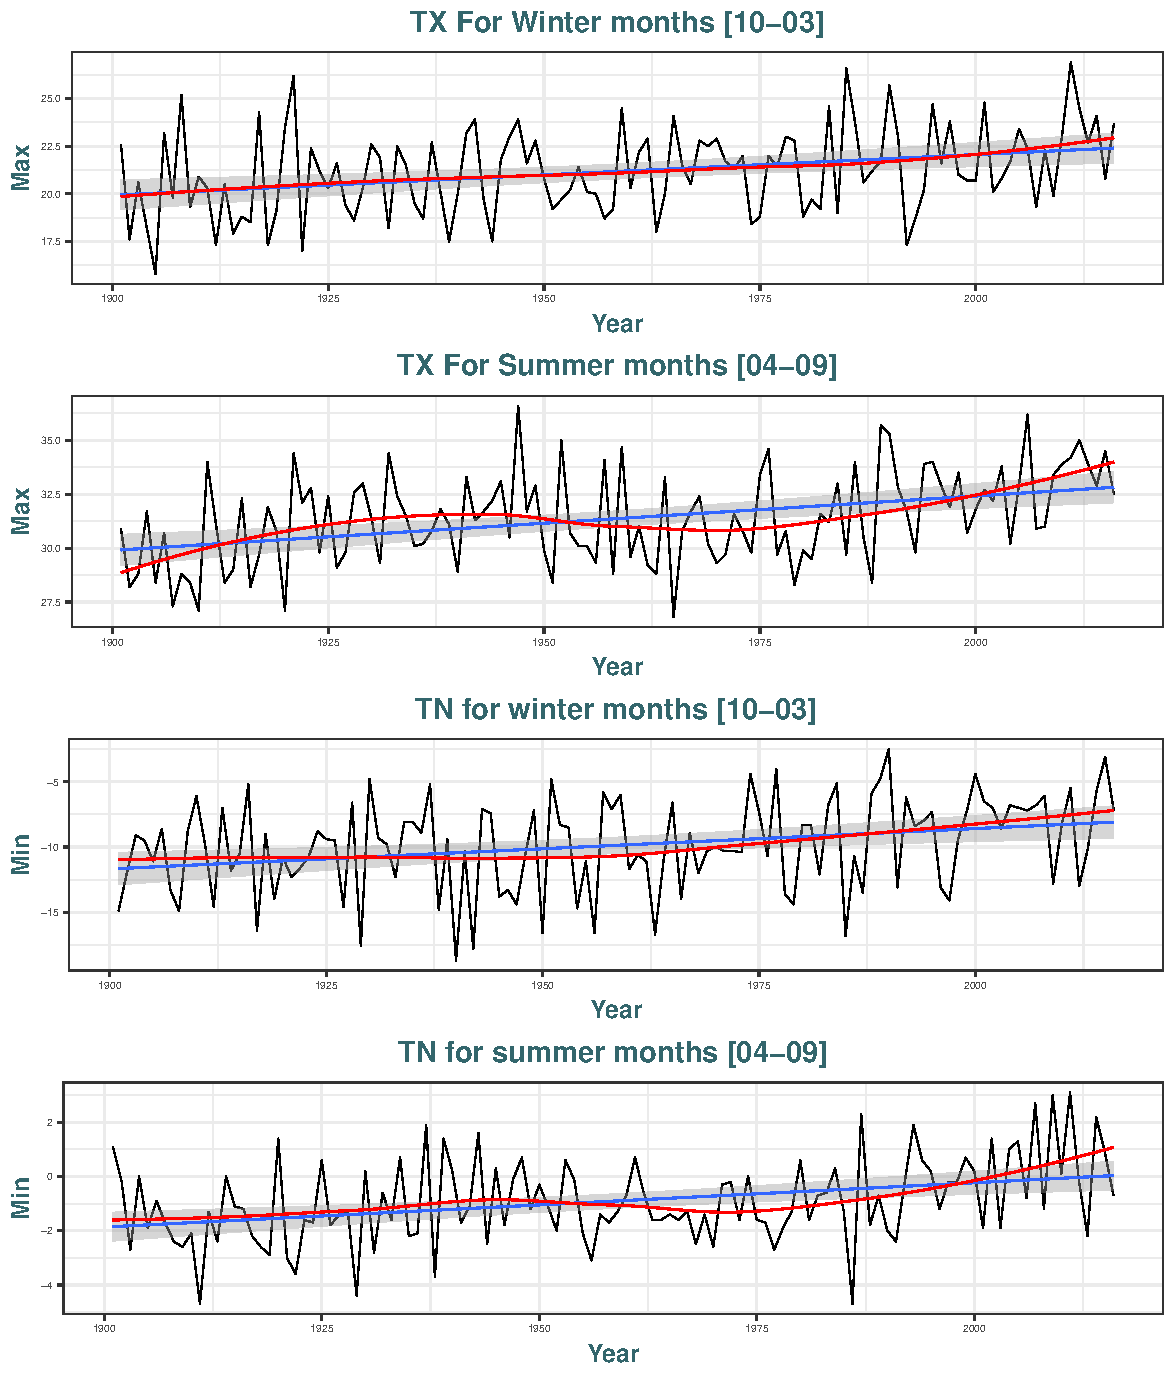
\includegraphics[width=\linewidth]{sumwint.pdf}\caption{First plot representing the \textbf{yearly} maxima (above) and minima (below) taking only the summer months (April to September) and winter months (October to March), shaded grey line around the linear trend represents its standard error. See how the polynomial trend (red line) also changes. Obv, TX for smummer and TN for winter are the same series as for the global serie}\label{seas4}

\end{figure}







\iffalse
\begin{figure}[!h]
	\minipage{\textwidth}
	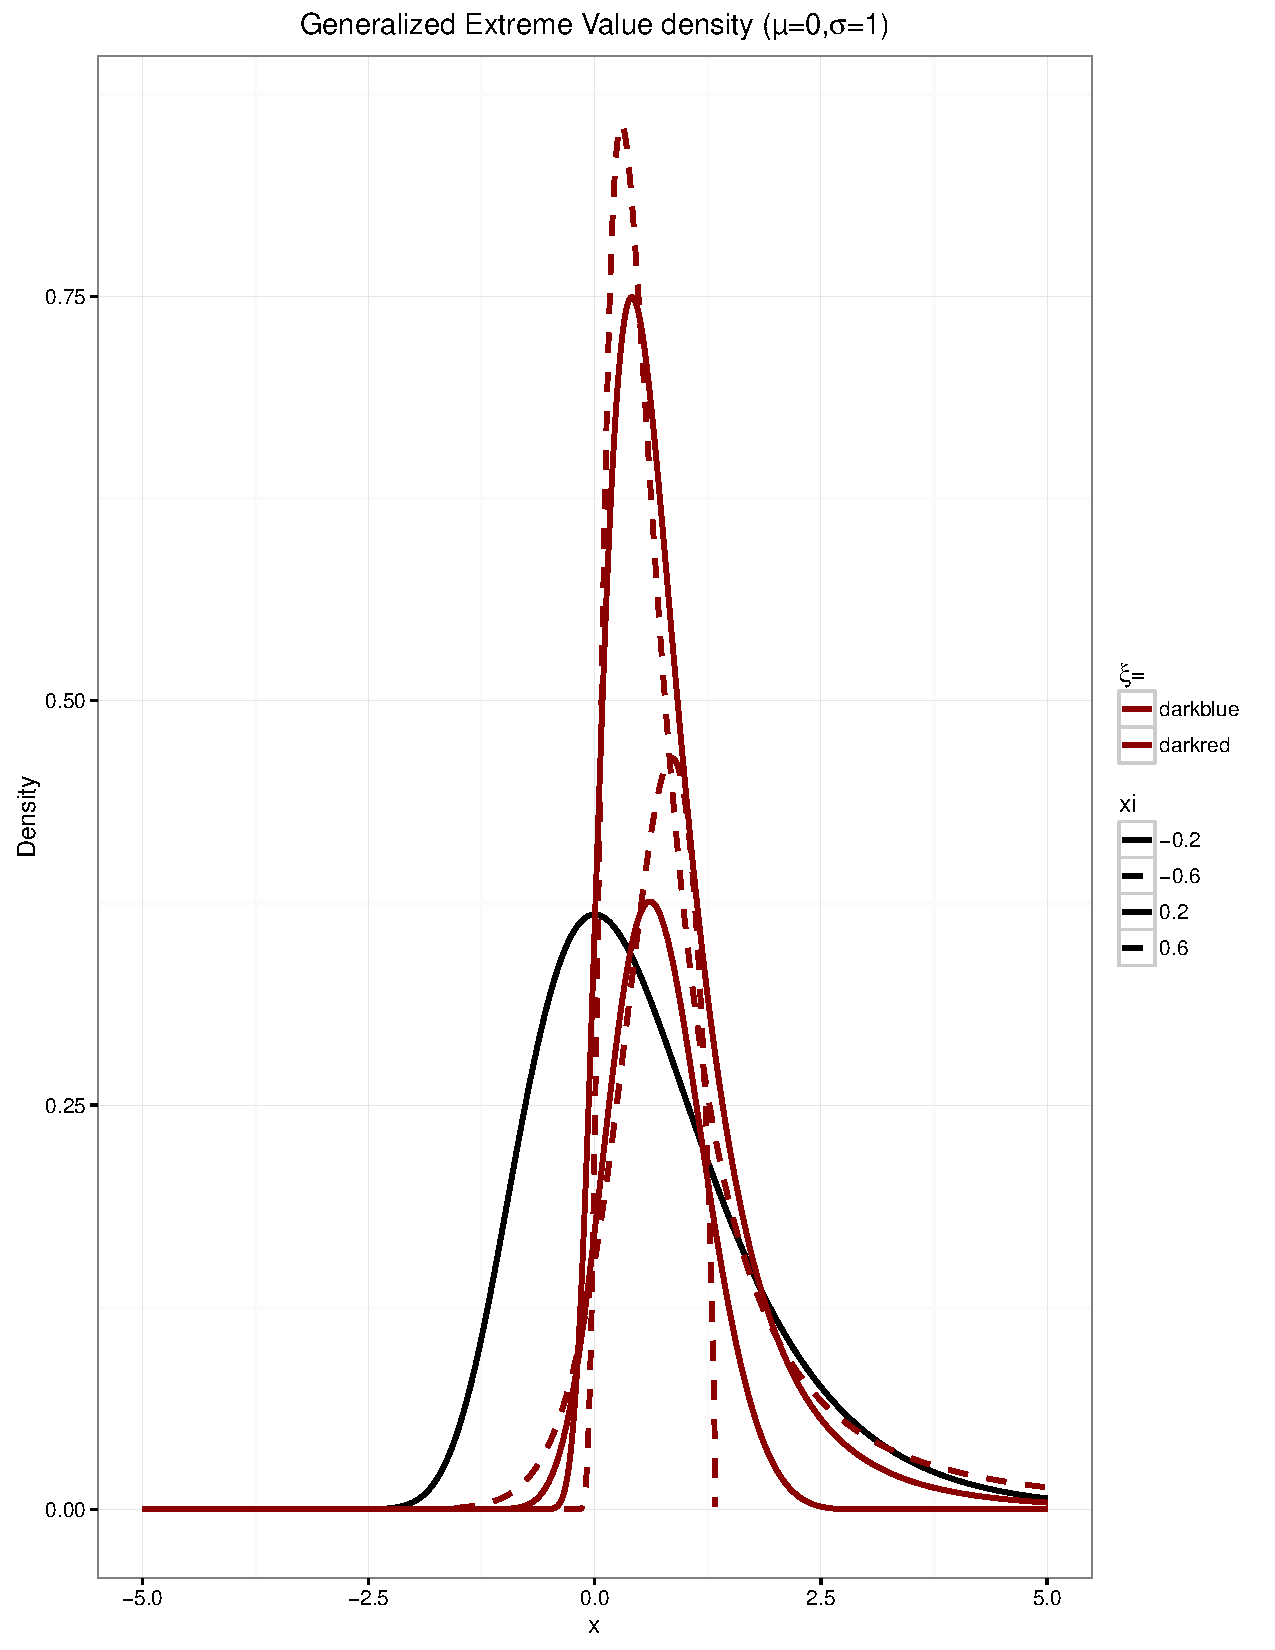
\includegraphics[width=\linewidth]{GEVV.pdf}
	\caption{ }\label{mcacls}
	\endminipage
\end{figure}
\begin{figure}[t!]
	$\begin{array}{rl}
	\multicolumn{2}{c}{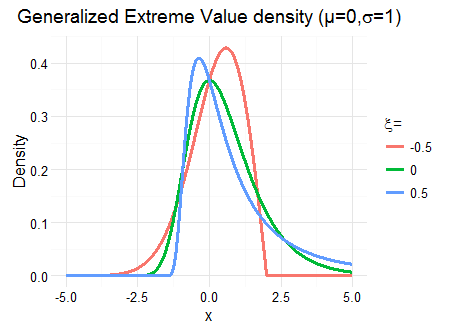
\includegraphics[width=0.85\textwidth]{GEV05.png}}\\
	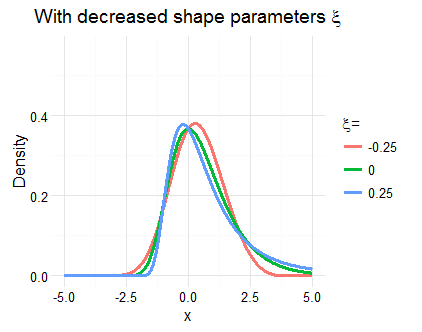
\includegraphics[width=0.5\textwidth]{GEV025.png} &
	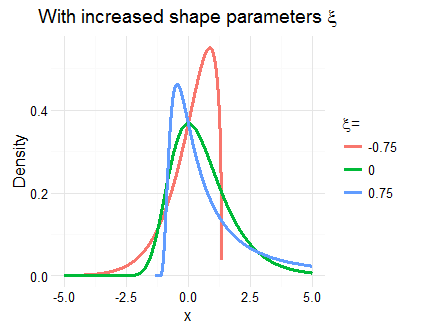
\includegraphics[width=0.5\textwidth]{GEV075.png}
	\end{array}$
	\caption{Representation of the GEV densities for various values of the shape parameter $\xi$ : $|\xi|=0.5$ (1) $|\xi|=0.25$, (2) and $|\xi|=0.75$ (3) for the Fréchet density [red], Weibull density [blue] while the Gumbel density [green] is kept fixed with $\xi=0$. }{\label{gevdens}}
\end{figure}
\fi 


\ do not forget \cite{emberchts_statistical_1997}

Beirlant: 2004 !!
%\nocite{}

%\bibliographystyle{abbrvnat}
\setlength{\parindent}{5em}
\setlength{\parskip}{2em}
\renewcommand{\baselinestretch}{4.0}

\bibliography{zotero.bib}
%\printbibliography

\end{document}